\documentclass[a4paper,oneside,11pt]{book}
\usepackage{CmBook}
\usepackage{graphics}
\usepackage{amsthm}
\lstdefinelanguage{cmpg}
{
	morekeywords={namespace,using,grammar,start,skip,token,keyword,keyword_list,empty,space,anychar,letter,digit,hexdigit,punctuation,var},
	sensitive=true,
	morecomment=[l]{//},
	morecomment=[s]{/*}{*/},
	morestring=[b]",
	morestring=[b]',
}
\theoremstyle{definition}
\newtheorem{exmp}{Example}[section]
\newtheorem{grmr}{Grammar}[section]
\newtheorem{algo}{Algorithm}[section]
\newtheorem{defn}{Definition}[section]
\begin{document}

\frontmatter
\title{Implementation of the Cmajor Compiler}
\author{Seppo Laakko}
\date{\today}
\maketitle
\tableofcontents

\mainmatter

\chapter{Introduction}

This document describes the implementation of the Cmajor compiler front-end.
We also inspect some excerpts of language theory and parsing theory as we go on
to make the description of implementation hopefully more understandable.

\section{Cmajor Programming Language and Cmajor Compilers}

Cmajor is a hybrid programming language that combines $\textrm{C}^\#$ like syntax with C++ like semantics.
The original Cmajor compiler is written in C++.
Now there is also a Cmajor compiler written in Cmajor that was created by manually converting
the C++ version to Cmajor. However it still lacks some features that are present in the C++ version, so the
the principal version as of this writing remains to be the C++ version.

\section{Phases of Compilation}

In classical compiler text books the compilation consists in principle of the following phases:

\begin{enumerate}

\item
In the lexical analysis phase a stream of characters of source code of a program is broken into lexical units called \emph{lexemes} and
an integer or enumerated value called a \emph{token} is assigned to each lexeme.

\item
In the syntax analysis phase the grammatical structure of tokens are analyzed, and \emph{abstract syntax trees} are generated.

\item
In the semantic analysis phase the syntax trees are traversed and the program is type-checked and verified that it consists
of semantically meaningful elements.

\item
In the intermediate code generation phase intermediate code for program elements are generated.

\item
In the machine-independent code optimization phase intermediate code is processed and optimized using various passes.

\item
In the code generation phase machine code is generated.

\item
In the machine-dependent code optimization phase the machine code is optimized further and target machine code is generated.

\end{enumerate}

The compiler collects information\footnote{type for example} about identifiers encountered in the program into a \emph{symbol table} and
consults the symbol table when information about an identifier is needed.

\begin{exmp}
Consider the following source code fragment:

\begin{lstlisting}
x = 10 * x + (cast<int>(c) - cast<int>('0'));
\end{lstlisting}

We are now going to have a taste of what the input and output of each phase of the compilation looks like.

\begin{enumerate}
\item
Lexical analysis. The lexical analyzer might produce the following lexemes for the code fragment above:
\begin{flushleft}
\verb|x|, \verb|=|, \verb|10|, \verb|*|, \verb|x|, \verb|+|, \verb|(|,
\verb|cast|, \verb|<|, \verb|int|, \verb|>|, \verb|(|, \verb|c|, \verb|)|, \verb|-|, \verb|cast|,
\verb|<|, \verb|int|, \verb|>|, \verb|(|, \verb|'0'| \verb|)|, \verb|)| and \verb|;|.
\end{flushleft}

If we represent punctuation and other symbolic lexemes with token values equal to themselves and
other lexemes with upper case identifiers, the lexical analyzer may assign the following tokens
to the lexemes that do not represent themselves:

\begin{itemize}
\item
\verb|x| : \textbf{ID} (identifier)
\item
\verb|10| : \textbf{INTLIT} (integer literal)
\item
\verb|cast| : \textbf{CAST} (reserved word)
\item
\verb|int| : \textbf{INT} (reserved word)
\item
\verb|c| : \textbf{ID} (identifier)
\item
\verb|'0'| : \textbf{CHARLIT} (character literal)
\end{itemize}

\item
Syntactic analysis.
The syntax analyzer or \emph{parser} receives the following
token stream from the lexical analyzer or \emph{lexer}:
\begin{flushleft}
\textbf{ID}, \verb|=|, \textbf{INTLIT}, \verb|*|, \textbf{ID}, \verb|+|, \verb|(|,
\textbf{CAST}, \verb|<|, \textbf{INT}, \verb|>|, \verb|(|, \textbf{ID}, \verb|)|, \verb|-|,
\textbf{CAST}, \verb|<|, \textbf{INT}, \verb|>|, \verb|(|, \textbf{CHARLIT}, \verb|)|,
\verb|)| and \verb|;|.
\end{flushleft}

The result of phase 2 is an abstract syntax tree or \emph{AST} that reveals
the syntactic structure of the source code.
Thus the parser may produce the following abstract syntax tree for the code fragment:

\begin{verbatim}
AssignmentStatementNode
    IdentifierNode(x)
    AddNode
        MulNode
            SByteLiteralNode(10)
            IdentifierNode(x)
        SubNode
            CastNode
                IntNode
                IdentifierNode(c)
            CastNode
                IntNode
                CharLiteralNode('0')
\end{verbatim}

\item
Semantic analysis. The abstract syntax trees generated in phase 2 are traversed and the
program is type-checked.
Assuming that identifier \verb|x| has been declared earlier to be a variable of type \textbf{int} and
identifier \verb|c| to be a variable of type \textbf{char},
the type-checker finds this information in the symbol table, when it walks the syntax tree.

When encountering the \verb|MulNode| the type-checker checks whether it is legal to multiply an \textbf{sbyte} literal 10 by
a variable \emph{x} of type \textbf{int}. This is the case so it records that the result of this multiplication produces a value
of type \textbf{int}.

When encountering the first \verb|CastNode| it checks if it is legal to convert a variable \emph{c} of type \textbf{char} to type \textbf{int}.
Similarly for the second \verb|CastNode|, the conversion of the character literal '0' to type \textbf{int} is checked.
They are both legal so the \verb|SubNode| produces a value of type \textbf{int}.

When encountering the \verb|AddNode| two \textbf{int} values are added and the result is of type \textbf{int}.

Finally when encountering the \verb|AssignmentStatementNode| the type-checker checks whether it is legal to assign a value of \textbf{int}
to a variable \verb|x| of type \textbf{int}. This is the case so the type-checking succeeds.

\item
Intermediate code generation.
The following intermediate code\footnote{this is LLVM intermediate code \cite{LLVM}}
may be produced from the abstract syntax tree and from information stored in the symbol table:

\begin{verbatim}
%1 = sext i8 10 to i32
%2 = load i32, i32* %x
%3 = mul i32 %1, %2
%4 = load i8, i8* %c
%5 = zext i8 %4 to i32
%6 = zext i8 48 to i32
%7 = sub i32 %5, %6
%8 = add i32 %3, %7
store i32 %8, i32* %x
\end{verbatim}

Quick introduction to intermediate instructions:

\begin{itemize}

\item
\verb|%1|, \verb|%2|, etc. represent intermediate results of computation.
They may be regarded as registers. There are inifinite number of them.

\item
\textbf{i8}, \textbf{i16} and \textbf{i32} are 8-bit, 16-bit and 32-bit integer types.

\item
\textbf{sext} instruction \emph{sign extends} its operand to a target type.

\item
\textbf{load} instruction loads a value of a variable.

\item
\textbf{mul} instruction multiplies two values.

\item
\textbf{zext} instruction \emph{zero extends} its operand to a target type.

\item
\textbf{sub} instruction subtracts a value from another.

\item
\textbf{add} instruction adds two values.

\item
\textbf{store} instruction stores a value to a variable.

\end{itemize}

\item
Code optimization. The following optimized intermediate code may be generated from the intermediate code produced in phase 4:

\begin{verbatim}
%1 = load i32, i32* %x
%2 = mul i32 %1, 10
%3 = load i8, i8* %c
%4 = zext i8 %3 to i32
%5 = add i32 %2, -48
%6 = add i32 %5, %4
store i32 %6, i32* %x
\end{verbatim}

\item
Machine code generation. The following fragment of assembly code may be generated:

\begin{verbatim}
movl	8(%rsp), %eax
leal	(%rax,%rax,4), %eax
movzbl	7(%rsp), %ecx
leal	-48(%rcx,%rax,2), %eax
movl	%eax, 8(%rsp)
\end{verbatim}

\section{Front-end and Back-end of a Compiler}

The lexical, syntactic and semantic analysis phases and intermediate code generation phase
form a \emph{front-end} of a compiler. The optimization and target machine code generation phases
form a \emph{back-end} of a compiler.

By combining $N$ programming language specific front-ends with $M$ target machine architecture specific back-ends
it is possible to create $N$ times $M$ compilers by writing only $N$ plus $M$ programs.

Intermediate code is the glue between the front and back ends of a compiler.

\section{Structure of This Document}

We begin by exploring the theory behind lexical analysis and continue with the practise of it in Cmajor compiler.
Next we go through some parsing theory to enlighten the syntax analysis phase and inspect the implementation of
Cmajor Parser Generator that is the parsing tool used in Cmajor compiler.
Finally we take some examples of implementation of the Cmajor language parser.

In the rest of this document we go through the semantic analysis and intermediate code generation that
are intertwined in the Cmajor compiler, and also go through other components of the compiler and other phases of
compilation that do not fit so nicely to the theory but are essential in any way.

\end{enumerate}
\end{exmp}

\chapter{Lexical Analysis}

The first phase of compilation is to break the character stream into tokens that are passed along to the parser.
Here a token is defined to be a name and an attribute value.
For example, \textbf{INTLIT} with a value 10.

Typically these tokens are described as \emph{patterns} that define the form
that the lexemes of a token may take. Here a lexeme is the actual sequence of
characters in an input stream that match that pattern.
One way to describe those patterns is to use \emph{regular expressions}.

\section{A Bit of Language Theory}

To describe regular expressions we take a small break and define a few fundamental concepts.

\subsection{Alphabets}

An \emph{alphabet} is a finite, nonempty set of symbols.
Conventionally, we use the symbol $\Sigma$ for an alphabet (\cite{AUTOMATA} pg. 28).

Typical alphabets are:
\begin{itemize}
\item
$\Sigma = \{0, 1\}$, a binary alphabet.

\item
$\Sigma = \{a, \ldots z\}$, the alphabet of lowercase latin letters.

\item
The set of ASCII characters.

\item
The set of Unicode characters.
\end{itemize}

\subsection{Strings}

A \emph{string} is a finite sequence of symbols chosen from some alphabet (\cite{AUTOMATA} pg. 29).
An \emph{empty string} is the string of zero occurrences of symbols. It is denoted $\epsilon$.

\subsubsection{Powers of an Alphabet}

If $\Sigma$ is an alphabet, we define $\Sigma^k$ to be the set of strings of length \emph{k}, each of whose
symbols is in $\Sigma$ (\cite{AUTOMATA} pg. 29).

Thus if $\Sigma = \{0, 1\}$, the binary alphabet:
\begin{itemize}
\item
$\Sigma^2$ = \{00, 01, 10, 11\}

\item
$\Sigma^3$ = \{000, 001, 010, 011, 100, 101, 110, 111\}
\end{itemize}

The set of all strings over an alphabet is denoted $\Sigma^*$.

\subsection{Languages}

A set of strings all of which are chosen from some $\Sigma^*$, where $\Sigma$ is a particular alphabet,
is called a \emph{language} (\cite{AUTOMATA} pg. 30).
If $\Sigma$ is an alphabet, and $L \subseteq \Sigma^*$, then $L$ is a language over $\Sigma$.

Examples of languages:
\begin{itemize}
\item
English: the collection of legal English words is a set of strings over the alphabet that consists of all
the letters.

\item
The language of legal C programs:
the alphabet is a subset of ASCII characters, and the language is a subset of all possible strings over
that alphabet.

\item
The set of binary numbers whose value is prime:
$$\{10, 11, 101, 111, 1011, \ldots\}$$

\item
$\emptyset$, the empty language, is a language over any alphabet.

\item
$\Sigma^*$ is a language over any alphabet.

\item
The language of all possible UTF-8 encoded strings of Unicode characters, denoted $L_{UTF8}$.

\item
The language of syntactically valid Cmajor programs, $L_{Cmajor} \subset L_{UTF8}$.
\end{itemize}

\subsection{Regular Expressions}

Regular expressions define languages.

Before describing the notation of regular expressions,
we need to define three operations on languages that the operators of regular expressions represent:

\begin{enumerate}

\item
The \emph{union} of two languages $L$ and $M$, denoted $L \cup M$, is the set of strings that are in
either $L$ or $M$, or both (\cite{AUTOMATA} pg. 84).
For example, if $L = \{01, 10\}$ and $M = \{10, 100\}$, $L \cup M = \{01, 10, 100\}$.

\item
The \emph{concatenation} of languages $L$ and $M$ is the set of strings that can be formed by taking
any string in $L$ and concatenating it with any string in $M$ (\cite{AUTOMATA} pg. 84).
We denote concatenation of $L$ and $M$ $LM$.
For example, if $L = \{01, 10\}$ and $M = \{10, 100\}$, $LM = \{0110, 01100, 1010, 10100\}$.

\item
The \emph{closure} of a language $L$, denoted $L^*$, is the infinite union $\cup _{i\ge0}L^i$,
where $L^0 = \{\epsilon\}$, the set containing the empty string, $L^1 = L$, and
$L^i$, for $i > 1$, is $LL \cdots L$, the concatenation of $i$ copies of $L$ (\cite{AUTOMATA} pg. 85).
For example, if $L = \{01, 10\}$, $L^* = \{\epsilon, 01, 10, 0101, 0110, 1010, \ldots\}$.
That is: $L^0$ gives $\{\epsilon\}$, the empty string, $L^1 = L$ gives $\{01, 10\}$;
$L^2 = LL$ gives $\{0101, 0110, 1001, 1010\}$ and so on.

\end{enumerate}

Now regular expressions can be defined recursively as follows:

\begin{flushleft}
\textbf{BASIS}: There are three parts:
\begin{enumerate}
\item
The constants $\epsilon$ and $\emptyset$ are regular expressions that denote languages $\{\epsilon\}$ and $\emptyset$ respectively.
That is, $L(\epsilon) = \{\epsilon\}$ and $L(\emptyset) = \emptyset$.

\item
If $a$ is any symbol, then \textbf{a}
is a regular expression \footnote{Here we denote regular expressions using \textbf{bold typeface} and symbols using \emph{italics}.}.
This regular expression denotes the language $\{a\}$.
That is, $L(\textbf{a}) = \{a\}$.

\item
A variable $L$ represents any language.
\end{enumerate}

\textbf{INDUCTION}: There are four parts:
\begin{enumerate}
\item
If $E$ and $F$ are regular expressions, then $E | F$ is a regular expression that denotes a union of $L(E)$ and $L(F)$.
That is, $L(E | F) = L(E) \cup L(F)$.

\item
If $E$ and $F$ are regular expressions, then $EF$ is a regular expression that denotes the concatenation of $L(E)$ and $L(F)$.
That is, $L(EF) = L(E)L(F)$.

\item
If $E$ is a regular expression, then $E^*$ is a regular expression that denotes the closure of $L(E)$. That is, $L(E^*) = (L(E))^*$.

\item
If $E$ is a regular expression, then $(E)$, a parenthesized regular expression, is also a regular expression,
that denotes the same language as $E$. That is, $L((E)) = L(E)$.

\end{enumerate}

\begin{exmp}

Let us use the formal theory to build a regular expression for sequence of one or more decimal digits.
First we use the basis rule 2 to build regular expressions for decimal digits:
$$\textbf{0}, \textbf{1}, \textbf{2}, \textbf{3}, \textbf{4}, \textbf{5}, \textbf{6}, \textbf{7}, \textbf{8}, \textbf{9}$$
Now we have languages $$L(\textbf{0}) = \{0\}, \ldots, L(\textbf{9}) = \{9\}$$

Next we use induction step 1 to build a regular expression for any decimal digit, denoted by $D$:
$$D = \textbf{0} | \textbf{1} | \textbf{2} | \textbf{3} | \textbf{4} | \textbf{5} | \textbf{6} | \textbf{7} | \textbf{8} | \textbf{9}$$
Now we have a language for a single decimal digit: $$L(D) = \{0, 1, \ldots, 9\}$$

Next we use induction step 3 to build a regular expression of any number, including zero, decimal digits:
$$E = D^*$$
Now we have a language for any number of decimal digits: $$L(E) = \{\epsilon, 0, 1, \ldots, 9, 00, 01, \ldots, 09, \ldots \}$$

Finally we exclude the empty string by concatenating one decimal digit with any number of decimal digits:
$$F = DD^*$$
The language for nonempty sequence of decimal digits is thus $$L(F) = \{0, 1, \ldots, 9, 00, 01, \ldots, 09, \ldots \}$$
\end{exmp}

\end{flushleft}

\clearpage

\section{Tools for Lexical Analysis}

Regular expressions can be used to describe patterns that form tokens.
But using regular expressions, one can describe only relatively simple kind of languages, namely \emph{regular languages}.

Strings that belong to a particular regular language can be recognized by constructing a \emph{finite automaton}.
A finite automaton is a kind of \emph{state machine}, it has states and transitions between the states,
but it has limited ``memory''. It cannot for example recognize the language of arbitrary long strings of balanced parentheses.

Many fundamental programming language constructs such as identifiers and literals are regular,
but to recognize potentially infinitely deep block structures, one needs to have a more powerful kind of language recognizer,
a finite automaton with a stack, or a \emph{pushdown automaton}.

A pushdown automaton can recognize a language that is
\emph{context-free}. The languages for syntactic structures in many programming languages are mostly context-free,
but for some constructs one may need to provide lexical information to guide the parser.

Finite automata can be constructed by hand, but there are also tools that take regular expression patterns as input and construct a
lexical analyzer that recognize those patterns. Such a tool is called a \emph{lexical-analyzer generator}.
Most famous is the Unix tool \verb|lex| and its GNU version \verb|flex|.

\clearpage
\section{Lexical Analysis in Cmajor}

The Cmajor compiler includes a tool called Cmajor Parser Generator, \verb|cmpg|, that combines the role of a parser generator and
a lexical-analyzer generator, or more truly, it is a parser generator that can be used without the need to have a separate
lexical-analyzer generator.

\subsection{Introduction to Cmajor Parser Generator}

The following table summarises some \verb|cmpg| expressions:

\begin{flushleft}
\begin{tabular}{lll}
\textbf{Expression}& \textbf{Matches}& \textbf{Example}\\
\hline
\textbf{empty}& empty string& \textbf{empty}\\
\textbf{space}& any white space character& \textbf{space}\\
\textbf{anychar}& any single character& \textbf{anychar}\\
\textbf{letter}& any latin letter& \textbf{letter}\\
\textbf{digit}& any decimal digit& \textbf{digit}\\
\textbf{hexdigit}& any hexadecimal digit& \textbf{hexdigit}\\
\textbf{punctuation}& any ASCII punctuation character& \textbf{punctuation}\\
'c'& character c& 'a'\\
$\backslash$c& character c literally& $\backslash$(\\
"s"& string s& "0x"\\
$[$s$]$& any one of characters in s& $[$abc$]$\\
$[$\verb|^|s$]$& any one character not in s& $[$\verb|^|abc$]$\\
$r*$& zero or more strings matching $r$& a*\\
$r+$& one or more strings matching $r$& a+\\
$r?$& zero or one r& a?\\
$r_1r_2$& an $r_1$ followed by an $r_2$& ab\\
$r_1 | r_2$& an $r_1$ or an $r_2$& a$|$b\\
$r_1 - r_2$& $r_1$ but not $r_2$& \textbf{anychar} $-$ "*/"\\
\hline
\end{tabular}
\end{flushleft}

To use \verb|cmpg|, one prepares \emph{.parser} files that contain \verb|cmpg| grammar definitions,
and a \emph{.pp} file that lists the \emph{.parser} files, and issues a command

\begin{verbatim}
cmpg file.pp
\end{verbatim}

The \verb|cmpg| reads and validates the grammar definitions in the \emph{.parser} files and
generates a C++ source and header files that contain C++ classes for each defined grammar.
When the resulting C++ source files are compiled and linked with \emph{Cm.Parsing} library,
the result is a top-down backtracking parser.

\clearpage
\subsection{Tokens in Cmajor}

We are now going to take a look of some classes of tokens in Cmajor programming language,
and how they are defined using \verb|cmpg| expressions.

\subsubsection{Skipping Whitespace and Comments}

We are not interested in contents of comments or whitespace during parsing, so they are skipped.
In a \verb|cmpg| grammar, one can define a \emph{skip} clause, to set a \emph{skip rule}
that is in effect during parsing. The parser alternates between parsing other tokens and skip tokens.
In the main compile unit grammar the skip rule is set to spaces_and_comments rule:

\begin{flushleft}
\begin{lstlisting}[language=cmpg,frame=trBL]
grammar CompileUnitGrammar
{
    // ...
    skip spaces_and_comments;
    // ...
}
\end{lstlisting}
\end{flushleft}

The \emph{spaces_and_comments} rule is defined here.
Note that the end of the block comment, "*/", is not matched
inside string or character literals.

\begin{flushleft}
\begin{lstlisting}[language=cmpg,frame=trBL]
spaces_and_comments
    ::= (space | comment)+
    ;

comment
    ::= line_comment | block_comment
    ;

line_comment
    ::= "//" [^\r\n]* newline
    ;

newline
    ::= "\r\n" | "\n" | "\r"
    ;

block_comment
    ::= "/*" (StringLiteral | CharLiteral | (anychar - "*/"))* "*/"
    ;
\end{lstlisting}
\end{flushleft}

\subsubsection{Identifiers and Keywords}

When parsing an identifier, for example, we must disable the skip rule.
Otherwise the parser would accept string ``iden ti fier'' as an identifier,
because whitespace is skipped.
For that, the \verb|cmpg| language has a \textbf{token} expression.
The \textbf{token} expression suppresses the skip rule when parsing the contents of the expression.

The difference expression, $r_1 - r_2$, matches $r_1$ but not $r_2$.
In this case $id\_chars - Keyword$ in line 2 rejects keywords as identifiers.

The \textbf{keyword\_list} expression in line 10 has two components.
The first is a name of a rule that selects a token, in this case $id\_chars$, and the
second is a list of keyword strings that are matched against the selected token.
If the selected token is found among the keyword strings,
the \textbf{keyword_list} expression accepts the selected token, otherwise it rejects it.

\begin{flushleft}
\begin{lstlisting}[language=cmpg,frame=trBL]
Identifier
    ::= token(id_chars - Keyword)
    ;

id_chars
    ::= token((letter | '_') (letter | digit | '_')*)
    ;

Keyword
    ::= keyword_list(id_chars,
        ["abstract", "and", "as", "axiom", "base", "bool", ...,
         "where", "while"])
    ;
\end{lstlisting}
\end{flushleft}

\subsubsection{Literals}

Literals in Cmajor, as in many other programming languages, can be parsed with regular expressions.

\begin{itemize}
\item
Let us start one of the simplest, a Boolean literal:

\begin{flushleft}
\begin{lstlisting}[language=cmpg,frame=trBL]
BooleanLiteral
    ::= keyword("true")
    |   keyword("false")
    ;
\end{lstlisting}
\end{flushleft}

The \textbf{keyword} expression matches the input to its parameter string,
but it accepts the input only if the input does \emph{not} continue with an identifier character:
a letter, a digit or an underscore.
If the \emph{BooleanLiteral} rule were defined using plain strings, like this:
\begin{flushleft}
\verb/BooleanLiteral ::= "true" | "false"/
\end{flushleft}
input like "truely" or "falsely" would be accepted as a \emph{BooleanLiteral} followed by "ly"
suffix. This is not what we want, so we use the \textbf{keyword} expression.

\item
Floating point numbers have many forms.
The \emph{fractional\_real} rule accepts inputs having a fractional part like
"1.23", ".987", "1.23e3" and "3.".
The \emph{exponent\_real} rule accepts decimal digits followed by exponent part like
"1e-2".

\begin{flushleft}
\begin{lstlisting}[language=cmpg,frame=trBL]
FloatingLiteral
    ::= token((fractional_real | exponent_real)('f' | 'F')?)
    ;

fractional_real
    ::= token(digit_sequence? '.' digit_sequence exponent_part?)
    |   token(digit_sequence '.')
    ;

digit_sequence
    ::= token(digit+)
    ;

sign
    ::= '+' | '-'
    ;

exponent_real
    ::= token(digit_sequence exponent_part)
    ;

exponent_part
    ::= token([eE] sign? digit_sequence)
    ;
\end{lstlisting}
\end{flushleft}

An optional 'f' or 'F' suffix denotes floating point literal that has type \textbf{float}.
Without the suffix floating point literals have type \textbf{double}.

\item
An integer literal can have either hexadecimal or decimal form.
The "0x" or "0X" prefix denotes hexadecimal integer literal.

\begin{flushleft}
\begin{lstlisting}[language=cmpg,frame=trBL]
IntegerLiteral
    ::= (hex_literal | digit_sequence) ('u' | 'U')?
    ;

hex_literal
    ::= token(("0x" | "0X") hex)
    ;

hex
    ::= token(hexdigit+)
    ;
\end{lstlisting}
\end{flushleft}

In Cmajor the type of an integer literal is the first of the of the following types in which its value can be represented:
\textbf{sbyte}, \textbf{byte}, \textbf{short}, \textbf{ushort}, \textbf{int}, \textbf{uint}, \textbf{long}, \textbf{ulong}.

The 'u' or 'U' suffix denotes an integer literal with an unsigned type. The type of it is the first of the following types
in which its value can be represented: \textbf{byte}, \textbf{ushort}, \textbf{uint}, \textbf{ulong}.

\item
The character literal rule accepts regular characters like 'a' or 'X', simple escapes like '$\backslash$n' and '$\backslash$r',
hexadecimal escapes like '$\backslash$xef', and decimal escapes  like '$\backslash$d100'.
Other escaped characters represent themselves.

\begin{flushleft}
\begin{lstlisting}[language=cmpg,frame=trBL]
CharLiteral
    ::= token('\'' ([^\\\r\n] | escape)'\'')
    ;

escape
    ::= token('\\' ([xX] hex | [dD] digit_sequence | [^dDxX]))
    ;
\end{lstlisting}
\end{flushleft}

\item
String literals can have four forms.

\begin{enumerate}
\item
Regular strings like "abc", or strings containing escaped characters like "line$\backslash$n".
The type of regular string literal is \textbf{const char*}.

\item
Wide strings like w"abc", or wide strings containing escapes. The type of wide string literal is \textbf{const wchar*}.

\item
Unicode strings like u"abc", or Unicode strings containing escapes. The type of Unicode string literal is \textbf{const uchar*}.

\item
Raw strings, that have @-prefix and have no escapes in them, like @"abc$\backslash$". The contents of raw string is taken literally.
The type of raw string literal is \textbf{const char*}.
\end{enumerate}

\begin{flushleft}
\begin{lstlisting}[language=cmpg,frame=trBL]
StringLiteral
    ::= string
    |   'w'string
    |   'u'string
    |   raw_string
    ;

string
    ::= token('"' (([^"\\\r\n]+) | escape)* '"')
    ;

raw_string
    ::= '@' token('"' [^"]* '"')
    ;
\end{lstlisting}
\end{flushleft}

\item
The last literal is the simplest, it's the null literal:

\begin{flushleft}
\begin{lstlisting}[language=cmpg,frame=trBL]
NullLiteral
    ::= keyword("null")
    ;
\end{lstlisting}
\end{flushleft}

\end{itemize}

\chapter{Syntax Analysis}

We are now going to explore a class of languages that are suitable for defining the grammatical structure of a programming language,
namely \emph{context-free languages}.
Context-free languages extend the notion of regular languages so that with a context-free language one can express also recursive
structures like nesting blocks or balanced parentheses.

\section{Example}

\begin{exmp}
A \emph{palindrome} is a string that reads the same forward or backward, such as \verb|otto| or
\verb|madamimadam| (``Madam, I'm Adam'', the first words that Adam said to Eve in the Garden of Eden.)
We can define palindromes for the binary alphabet, $\Sigma = \{0, 1\}$, recursively as follows:

\begin{flushleft}
\textbf{BASIS}\\
$\epsilon$, i.e. the empty string, $0$, and $1$ are palindromes.
\end{flushleft}

\begin{flushleft}
\textbf{INDUCTION}\\
If $P$ is a palindrome, so are $0P0$ and $1P1$. No string is a palindrome of 0's and 1's unless it follows from this basis and induction rule.
\end{flushleft}

A context-free grammar is a formal notation for expressing such recursive definitions of languages (\cite{AUTOMATA} pg. 170).
A grammar consists of one or more variables that represent classes of strings, i.e. languages. In previous example we have only one variable, $P$,
which represents the set of palindromes; that is the class of strings forming the language $L_{pal}$. There are rules that say how the strings in
each class are constructed. The construction can use symbols of the alphabet, strings that are known to be in one of the classes, or both.

\begin{grmr}\label{pgram}
The rules that define the palindromes, expressed in the context-free grammar notation, are:
\begin{align}
P &\rightarrow \epsilon\\
P &\rightarrow 0\\
P &\rightarrow 1\\
P &\rightarrow 0P0\\
P &\rightarrow 1P1
\end{align}
\end{grmr}

The first three rules form the basis. They tell us that a class of palindromes includes the strings $\epsilon$, $0$, and $1$.
None of the right sides of these rules contains a variable, which is why they form a basis for the definition.

The last two rules form the inductive part of the definition. For instance, rule 3.4 says that if we take any string $\omega$ from the class $P$,
then $0\omega0$ is also in class $P$. Rule 3.5 likewise tells us that $1\omega1$ is also in class $P$.
\end{exmp}

\section{Definition of Context-Free Grammars}

There are four important components in a grammatical description of a language (\cite{AUTOMATA} pg. 171):

\begin{enumerate}

\item
There is a finite set of symbols that form the strings of the language being defined. This set was $\{0, 1\}$ in the palindrome example.
We call this alphabet the \emph{terminals}, or \emph{terminal symbols}.

\item
There is a finite set of \emph{variables}, sometimes called \emph{nonterminals}. Each variable represents a language; i.e. a set of strings.
In the last example, there was only one variable, $P$, which we used to represent the class of palindromes over alphabet $\{0, 1\}$.

\item
One of the variables represents the language being defined; it is called the \emph{start symbol}. Other variables represent auxiliary classes of
strings that are used to help define the language of the start symbol. In our example, $P$, the only variable, is the start symbol.

\item
There is a finite set of \emph{productions} or \emph{rules} that represent the recursive definitiion of the language.
Each production consists of:
\begin{enumerate}
\item
A variable that is being (partially) defined by the production. This variable is often called the \emph{head} of the production.

\item
The production symbol $\rightarrow$.

\item
A string of zero or more terminals and variables. This string, called the \emph{body} of the production,
represents one way to form strings in the of the variable of the head. In doing so, we leave terminals unchanged and substitute for each variable
of the body any string that is known to be in the language of that variable.
\end{enumerate}
\end{enumerate}

We follow a convention that if the start symbol is not explicitly specified, the head of the first production of the grammar is the start symbol.

\subsection{Derivations Using a Grammar}

To infer that a certain string is in the language of a grammar, we start with the start symbol of the grammar
and expand it using one of its productions, i.e. by replacing the head of the production with its body.
Then we further expand the resulting string by replacing one of its variables by the body of one of its productions,
and so on, until we derive a string consisting entirely of terminals. The language of the is all strings of terminals that
we can obtain this way. This use of grammar is called a \emph{derivation}.

To see that string 0110 is in the language of binary palindromes $L_{pal}$, for example, we start from the start symbol $P$,
and replace it with the body of the production 4 of grammar \ref{pgram}: $P \Rightarrow 0P0$. We then replace the variable $P$ between the 0's with
the body of the production 5: $0P0 \Rightarrow 01P10$. Finally we replace the variable $P$ in the obtained string with
the body of the production 1: $01P10 \Rightarrow 01 \epsilon 10$.
That way we have the derivation $P \Rightarrow 0P0 \Rightarrow 01P10 \Rightarrow 0110$ and we have inferred that
$0110 \in L_{pal}$.

We denote that there is a derivation that requires zero or more derivation steps with $\overset{*}{\Rightarrow}$ symbol.
For example, to indicate that there is a derivation of string $0110$ from variable $P$ using some number of steps,
is denoted $P \overset{*}{\Rightarrow} 0110$.

\subsection{Parse Trees for a Grammar}

There is a tree representation for derivations that show explicitly how terminal symbol are grouped into substrings,
each of which belongs to the language of one of the variables of the grammar. These trees are called \emph{parse trees}.
There might be more than one parse tree for a terminal string that belongs to the language of some grammar.
In that case the grammar is called \emph{ambiguous}. Ambiguous grammars are not suitable for representing a syntax
of a programming language unless the ambiguities are resolved somehow.

The parse trees of a specific grammar G are trees with the following conditions:

\begin{enumerate}
\item
Each interior node is labeled by a variable of the grammar.

\item
Each leaf is labeled by either a variable, a terminal, or $\epsilon$.
However, if the leaf is labeled $\epsilon$, then it must be the only child of its parent.

\item
If an interior node is labeled $A$, and its children are labeled
$$X_1, X_2, \ldots, X_k$$

respectively, from the left, then $A \rightarrow X_1 X_2 \cdots X_k$ is a production of the grammar $G$.
\end{enumerate}

Figure \ref{fig:parsetree} shows a parse tree of derivation $P \overset{*}{\Rightarrow} 0110$ for the
grammar \ref{pgram}.

\begin{figure}[htb]
\caption{A parse tree for derivation $P \overset{*}{\Rightarrow} 0110$ }
\label{fig:parsetree}
\vspace{0.5cm}
\begin{center}
\includegraphics{parsetree}
\end{center}
\end{figure}

\subsection{Compact Notation for Grammars}

Let $\omega_1, \omega_2, \ldots, \omega_k$ be strings of grammar symbols (i.e. strings of terminals and nonterminals).
If we have productions

\begin{align*}
P &\rightarrow \omega_1\\
P &\rightarrow \omega_2\\
&\ldots\\
P &\rightarrow \omega_k\\
\end{align*}

in some grammar G, we may represent the $P$-productions (i.e. the productions whose head is $P$) by grouping them together as follows:

\begin{flushleft}
$P \rightarrow \omega_1\, | \, \omega_2 \, | \, \cdots \, | \, \omega_k$
\end{flushleft}

For example, the grammar \ref{pgram} may be represented more compactly as
$$P \rightarrow \epsilon \, | \, 0 \, | \, 1 \, | \, 0P0 \, | \, 1P1$$

\clearpage

\section{Syntax-Directed Translation}

Consider the following grammar:

\begin{grmr}\label{g:infix}
\begin{align*}
expr &\rightarrow expr + term\, |\, expr - term \,| \, term\\
term &\rightarrow term * factor\, |\, term / factor \, | \, factor\\
factor &\rightarrow 0\,|\,1\,|\,2\,|\,3\,|\,4\,|\,5\,|\,6\,|\,7\,|\,8\,|\,9\,|\,(\, expr \,)
\end{align*}
\end{grmr}

The language defined by this grammar consists of expressions that are lists of terms separated by
operator symbols $+$ and $-$. Terms are in turn lists of factors separated by operator symbols $*$ and $/$.
Factors consist of single digits and parenthesized expressions.
The alphabet of this language is $\{+, -, *, /, 0, 1, 2, 3, 4, 5, 6, 7, 8, 9, (, ) \}$.

To see that an expression "1+3*(4-2)", for example, is in this language, we may construct a
derivation for it:

\begin{align*}
expr &\Rightarrow expr + term\\
&\Rightarrow term + term\\
&\Rightarrow factor + term\\
&\Rightarrow 1 + term\\
&\Rightarrow 1 + term * factor\\
&\Rightarrow 1 + factor * factor\\
&\Rightarrow 1 + 3 * factor\\
&\Rightarrow 1 + 3 * ( expr )\\
&\Rightarrow 1 + 3 * ( expr - term )\\
&\Rightarrow 1 + 3 * ( term - term )\\
&\Rightarrow 1 + 3 * ( factor - term )\\
&\Rightarrow 1 + 3 * ( 4 - term )\\
&\Rightarrow 1 + 3 * ( 4 - factor )\\
&\Rightarrow 1 + 3 * ( 4 - 2 )\\
\end{align*}

Suppose now that we need to translate infix expressions of this kind into \emph{postfix notation}.
The postfix notation of an expression $E$ can be defined inductively as follows:

\begin{enumerate}
\item
If $E$ is a digit, the postfix notation of $E$ is $E$ itself.
\item
If $E$ is of the form $E_1 + E_2$, the postfix notation of $E$ is the postfix notation of $E_1$ followed by the postfix notation of $E_2$ followed by +.
\item
If $E$ is of the form $E_1 * E_2$, the postfix notation of $E$ is the postfix notation of $E_1$ followed by the postfix notation of $E_2$ followed by *.
\item
If $E$ is of the form $(E)$, the postfix notation of $(E)$ is the postfix notation of $E$.
\end{enumerate}

For example, postfix notation for infix expression "1+3*(4-2)" is "1342-*+".

In computing the postfix notation from infix expressions, we can take advantage of the grammar \ref{g:infix} by associating
\emph{attributes} to each nonterminal of the grammar. Attributes can in principle be of any kind: numbers, structures or strings, for example.
In this case we may represent the value of a postfix expression with one string attribute.
A parse tree that shows the values of the attributes of nonterminals is called an \emph{annotated} parse tree.

Figure \ref{fig:annotated} shows an annotated parse tree with an attribute \emph{pf} associated with nonterminals $expr$, $term$ and $factor$.

\begin{figure}[htb]
\caption{Annotated parse tree for expression "1+3*(4-2)"}
\label{fig:annotated}
\vspace{0.5cm}
\begin{center}
\includegraphics{annotated}
\end{center}
\end{figure}

There can be two kinds of attributes for nonterminals: (\cite{COMPILERS} pg. 304)

\begin{enumerate}
\item
A \emph{synthesized attribute} for a nonterminal $A$ at a parse-tree node $N$ is defined by a semantic action associated with the production at $N$.
A synthesized attribute at node $N$ is defined in terms of attribute values at the children of $N$ and at $N$ itself.
The \emph{pf} attribute in Fig. \ref{fig:annotated} is an example of a synthesized attribute.

\item
An \emph{inherited attribute} for a nonterminal $B$ at a parse-tree node $N$ is defined by a semantic action associated with the production at the
\emph{parent} of $N$. An inherited attribute at node $N$ is defined in terms of attribute values at $N$'s parent, $N$ itself, and $N$'s siblings.
\end{enumerate}

The attributes can be computed by visiting the nodes of the parse tree in some order.
Synthesized attributes have the nice property that their values can be computed by a single bottom-up travelsal of the parse tree.

\section{Parsing}

Parsing is the process of determining how a string of terminals can be generated by a grammar. (\cite{COMPILERS} pg. 60).
Most parsing methods fall into one of two classes, called the \emph{top-down} and \emph{bottom-up} methods.
These terms refer to the order in which nodes in the parse tree are constructed. In top-down parsers,
construction starts at the root and proceeds towards the leaves, while in  bottom-up parsers, construction starts the the
leaves and proceeds towards the root. Most handwritten parsers use top-down methods, while many parser-generator tools
generate a bottom-up parser.

\subsection{Recursive Descent Parsing}

A \emph{recursive-descent parsing} is a top-down method in which a set of recursive procedures is used to process the input.
For example, consider the following grammar:

\begin{grmr}\label{g:if}
$$
stmt \rightarrow \textbf{if} \, \textbf{(} \, expr \, \textbf{)} \, stmt \, \textbf{else} \, stmt
$$
\end{grmr}

To write a recursive-descent parser for this grammar, one writes a procedure that is used to match tokens and obtain more input,
and then a procedure for each nonterminal.
The following listing shows the structure of these procedures:

\begin{lstlisting}[language=C++]
int lookahead;

void match(int token)
{
    if (token == lookahead)
    {
        // read next token into lookahead;
    }
    else
    {
        throw std::runtime_error("syntax error");
    }
}

void expr()
{
    // match an expression...
}

void stmt()
{
    match(IF); match('('); expr(); match(')'); stmt(); match(ELSE); stmt();
}

\end{lstlisting}

\clearpage
\subsection{Left Recursion}

A recursive-descent parser cannot directly use grammars like the grammar \ref{g:infix}, because it has ``left-recursive'' productions
such as $expr \rightarrow expr + term$, where the leftmost symbol of the body is the same as the nonterminal at the head of
the production. Suppose the procedure for \emph{expr} decides to apply this production. The body begins with \emph{expr} so
the procedure for \emph{expr} is called recursively. Since the lookahead symbol changes only when a terminal is matched,
no change to the input took place between recursive calls of \emph{expr}. As a result, the second call to \emph{expr} does
exactly what the first call did, which means a third call, and so on.

A left-recursive production can be eliminated by rewriting the offending production.
Consider a nonterminal $A$ with two productions $$A \rightarrow A\alpha \,|\, \beta$$
where $\alpha$ and $\beta$ are sequences of terminals and nonterminals that do not start with $A$.
For example, in $$expr \rightarrow expr + term \, | \, term$$ nonterminal $A = expr$, string $\alpha = + term$, and string $\beta = term$.

The nonterminal $A$ and its production are said to be \emph{left recursive} (\cite{COMPILERS} pg. 67), because the production $A \rightarrow A\alpha$
has $A$ itself as the leftmost symbol of the right side. Repeated application of this production builds up a sequence of $\alpha$'s
to the right of $A$. When $A$ is finally replaced by $\beta$, we have a $\beta$ followed by a sequence of zero or more $\alpha$'s.

We can achieve the same effect by rewriting the productions for $A$ in the following manner, using a new nonterminal $R$:
\begin{align*}
A &\rightarrow \beta R\\
R &\rightarrow \alpha R \,|\, \epsilon
\end{align*}


\section{Extending the Grammar Notation}

We have found it useful to extend the context-free grammar notation with regular-expression like operations.
\footnote{$\alpha$ and $\beta$ denote strings of grammar symbols, and $X$ and $Y$ single grammar symbols.}
\footnote{Since asterisk, plus, question mark, parentheses and square brackets belong to regular expression syntax,
they must now be quoted when they appear as terminals in productions of extended notation.}
In the following definitions the expression in the middle is in the extended form, and the productions on the right
express the same language using conventional context-free grammar notation.

\begin{enumerate}
\item X or Y:
\begin{align*}
P &\rightarrow \alpha\, (X\,|\,Y)\, \beta & P &\rightarrow \alpha R \beta\\
  &                             & R & \rightarrow \, X \, | \, Y
\end{align*}
\item Closure of $X$, $X$ occurs zero or more times:
\begin{align*}
P &\rightarrow \alpha X^* \beta & P &\rightarrow \alpha R \beta\\
  &                             & R & \rightarrow RR\, | \, X \, | \, \epsilon
\end{align*}
\item Positive $X$, $X$ occurs one or more times:
\begin{align*}
P &\rightarrow \alpha X^+ \beta & P &\rightarrow \alpha R \beta\\
  &                             & R & \rightarrow RR\, | \, X
\end{align*}
\item Optional $X$, $X$ occurs zero or one times:
\begin{align*}
P &\rightarrow \alpha X? \beta & P &\rightarrow \alpha R \beta\\
  &                            & R & \rightarrow X \,|\, \epsilon
\end{align*}
\item Class [abc], one of the characters in the class occurs:
\begin{align*}
P & \rightarrow \alpha \, [abc] \, \beta & P &\rightarrow \alpha R \beta\\
  &                            & R & \rightarrow a \,|\, b \, | \, c
\end{align*}
\end{enumerate}

In the definitions above, $X$ denotes a single grammar symbol, i.e. either terminal or nonterminal,
but we may extend the notation further by substituting $X$ with arbitrary expressions containing
grammar symbols and other expressions, much the same way we can use regular expressions.
We can now replace left recursion with iteration using the extended notation.
The left-recursive productions
$$A \rightarrow A\alpha \,|\, \beta$$
become an iterative production:
$$A \rightarrow \beta (\alpha)^*$$
meaning $\beta$ followed by zero or more $\alpha$'s.

We can rewrite the grammar \ref{g:infix} without left recursion using the extended notation as follows:

\begin{grmr}\label{g:expr}
\begin{align*}
expr &\rightarrow term \>(\>('+'|'-')\> term \>)^*\\
term &\rightarrow factor \>(\>('*'|'/')\> factor \>)^*\\
factor &\rightarrow [0-9] \> |\> '('\> expr \> ')'
\end{align*}
\end{grmr}

\section{Parsing in Cmajor}

The parsers in Cmajor are written using the Cmajor Parser Generator, or \verb|cmpg|, notation,
that is much like the extended grammar notation of the previous section.
The \verb|cmpg| reads grammar definitions in \emph{.parser} files, validates them,
and generates C++ classes that represent the grammars. To become familiar with the grammar definition syntax,
we write the grammar \ref{g:expr} using the \verb|cmpg| notation.

\clearpage
\begin{exmp} Postfix Translation Grammar.\label{ex:postfix}
\lstset{language=cmpg}
\begin{lstlisting}
grammar PostfixTranslationGrammar
{
    expr: std::string
        ::= term:t{ value = t; }
        (   '+' term:pt{ value.append(pt).append(1, '+'); }
        |   '-' term:mt{ value.append(mt).append(1, '-'); }
        )*
        ;

    term: std::string
        ::= factor:f{ value = f; }
        (   '*' factor:tf{ value.append(tf).append(1, '*'); }
        |   '/' factor:df{ value.append(df).append(1, '/'); }
        )*
        ;

    factor: std::string
        ::= digit{ value = std::string(1, *matchBegin); }
        |   '(' expr{ value = expr; } ')'
        ;
}
\end{lstlisting}

The grammar has a list of \emph{rules}. In this case \emph{expr}, \emph{term} and \emph{factor}.
If the start rule is not explicitly defined by the \textbf{start} clause, the first rule of the grammar
is taken as the start rule.

A rule may have one synthesized attribute whose type is denoted by a colon and a name of a C++ type after
the head of the rule, \verb|std::string| in this case. In this example each of the rules of the grammar have a
synthesized attribute of type \verb|std::string|.
If multiple synthesized attributes are needed, one can specify a structure of values,
or a dynamically created object holding the values.

The ::= symbol corresponds to the $\rightarrow$ symbol in the formal grammars.

If the same nonterminal occurs many times inside the body of a rule, and that nonterminal refers to a rule that has a synthesized attribute,
the synthesized attribute has to be named explicitly by a colon and an identifier after the name of the nonterminal.
In the body of the \emph{expr} rule, for example, one can refer to many occurrences of \emph{term}'s synthesized attribute,
the first of which is named \emph{t}, the second \emph{pt}, and the third \emph{mt}.

A grammar symbol in a body of a rule may have an associated semantic action, i.e. a block of C++ code.
For example in line 4, the first \emph{term} nonterminal has a semantic action \verb|{ value = t; }| associated with it.
The semantic action is executed only if input matches the rule that it is associated with.

The synthesized attribute of the rule is exposed as an identifier \emph{value} inside the body of a rule.
It can be read and assigned to many times inside the body of a rule.
For example in line 4, the value of the synthesized attribute of the \emph{expr} rule is initialized to a value of the synthesized attribute of the
\emph{term} rule. When more \emph{term}s are matched, the synthesized attributes of these are appended to the synthesized attribute the \emph{expr} rule.

The matched lexeme of a grammar symbol is exposed as two character pointers to the semantic action associated with a grammar symbol.
The \emph{matchBegin} pointer points to the start of the matched lexeme and the \emph{matchEnd} pointer points to one past the end of the matched lexeme.
For example, in line 18, the value of the matched digit is assigned to the synthesized attribute of the \emph{factor} rule.

If the nonterminal occurs only once inside the body of a rule, one can refer the synthesized attribute of it with the name of the nonterminal.
Example of this appears in the line 19, where the synthesized attribute of \emph{expr} rule is referred in the semantic action by its name \emph{expr}.
\end{exmp}

\subsection{Internal Representation of \texttt{cmpg} Grammar Definitions}

The \verb|cmpg| program reads grammar definitions and constructs an internal representation for them.
The internal representation of a grammar is a list of rules, one of which is set as a start rule.
Each rule has a \emph{name} and a \emph{definition}.
The definition of a rule is represented as a \emph{tree of parsing nodes}.

There are many kinds of parsing nodes. Each kind of parsing node has either zero, one, or two child nodes.
A node that has zero child nodes is also called a \emph{leaf} parsing node,
a node that has one child node is called a \emph{unary} parsing node,
and a node that has two child nodes is called a \emph{binary} parsing node.

\begin{itemize}

\item
The definition of a rule consists of nonempty sequence of \emph{alternative} expressions:

$$R \rightarrow \omega_1 \, | \, \omega_2 \, | \, \cdots \, | \, \omega_k$$

If input matches one of the alternatives, it matches the rule.
The alternatives are tested from left to right, and if a match is found, the rest of the alternatives are not tested.

If the definition of a rule is represented as a tree of parsing nodes, it consists of \emph{alternative} binary parsing nodes,
where the left and right subtrees of an alternative nodes represent expressions $\omega_i$ and $\omega_{i + 1}$.
Figure \ref{fig:alternatives} shows two alternative nodes.

\begin{figure}[htb]
\caption{Alternative Nodes}
\label{fig:alternatives}
\vspace{0.5cm}
\begin{center}
\includegraphics{alternatives}
\end{center}
\end{figure}

\item
Each alternative expression $\omega_i$ consists of catenation of expressions :

$$\alpha_1 \alpha_2 \cdots \alpha_k$$

If input consists of a nonempty sequence of strings $s_1, s_2, \ldots, s_k$ of terminal symbols where $s_1$ matches expression $\alpha_1$,
$s_2$ matches expression $\alpha_2$, etc., and $s_k$ matches expression $\alpha_k$,
the input matches the whole alternative expression.

A \emph{catenate} node is a binary parsing node, whose left and right subtree represent expressions $\alpha_i$ and $\alpha_{i + 1}$.
Figure \ref{fig:catenate} shows two catenate nodes.

\begin{figure}[htb]
\caption{Catenate Nodes}
\label{fig:catenate}
\vspace{0.5cm}
\begin{center}
\includegraphics{sequences}
\end{center}
\end{figure}

\item
A \emph{difference} expression is denoted by $\alpha_i$ in a catenate expression $\alpha_1 \alpha_2 \cdots \alpha_k$.
The difference expression consists of nonempty sequence of expressions separated by the $-$ symbol:

$$\beta_1 \,-\, \beta_2 \,-\, \cdots \,-\, \beta_k$$

Usually $k=1$ or $k=2$.
If a string $s$ of terminal symbols matches expression $\beta_1$, but does not match expression $\beta_2$,
the string $s$ matches expression $\beta_1 - \beta_2$.

A \emph{difference} node is a binary parsing node whose left and right subtrees represent expressions $\beta_1$ and $\beta_2$ respectively.
Figure \ref{fig:difference} shows a difference node.

\begin{figure}[htb]
\caption{Difference Node}
\label{fig:difference}
\vspace{0.5cm}
\begin{center}
\includegraphics{difference}
\end{center}
\end{figure}

\item
An \emph{xor} expression is denoted by $\beta_i$ in a difference expression $\beta_1 \,-\, \beta_2 \,-\, \cdots \,-\, \beta_k$.
The xor expression consists of nonempty sequence of expressions separated by the $\hat{}$ symbol:

$$\gamma_1 \, \hat{} \, \gamma_2\, \hat{} \, \cdots \, \hat{} \, \gamma_k$$

Usually $k=1$ or $k=2$.
If a string $s$ of terminal symbols either matches expression $\gamma_1$, but does not match expression $\gamma_2$,
or matches expression $\gamma_2$, but does not match expression $\gamma_1$, the string $s$ matches expression $\gamma_1\, \hat{}\, \gamma_2$.

An \emph{xor} node is a binary parsing node whose left and right subtrees represent expressions $\gamma1$ and $\gamma2$ respectively.
Figure \ref{fig:xor} shows an xor node.

\begin{figure}[htb]
\caption{Xor Node}
\label{fig:xor}
\vspace{0.5cm}
\begin{center}
\includegraphics{xor}
\end{center}
\end{figure}

\item
An \emph{intersection} expression is denoted by $\gamma_i$ in an xor expression $\gamma_1 \, \hat{} \, \gamma_2\, \hat{} \, \cdots \, \hat{} \, \gamma_k$.
The intersection expression consists of nonempty sequence of expressions separated by the $\&$ symbol:

$$\mu_1 \, \& \, \mu_2 \, \& \, \cdots \, \& \mu_k$$

Usually $k = 1$ or $k = 2$.
If a string $s$ of terminal symbols matches both expression $\mu_1$ and expression $\mu_2$, the string $s$ matches expression $\mu_1 \& \mu_2$.

An \emph{intersection} node is a binary parsing node whose left and right subtrees represent expressions $\mu_1$ and $\mu_2$ respectively.
Figure \ref{fig:and} shows an intersection node.

\begin{figure}[htb]
\caption{Intersection Node}
\label{fig:and}
\vspace{0.5cm}
\begin{center}
\includegraphics{and}
\end{center}
\end{figure}

\clearpage
\item
A \emph{list} expression is denoted by $\mu_i$ in an intersection expression $\mu_1 \, \& \, \mu_2 \, \& \, \cdots \, \& \mu_k$:
The list expression is an expression optionally followed by the $\%$ symbol and an expression:

$$\theta_1 \, (\% \, \theta_2)?$$

In the previous expression the parentheses and the $?$ symbol are metasymbols, not terminal symbols.

Expression $\theta_1 \% \theta_2$ denotes a nonempty sequence of $\theta_1$'s separated by $\theta_2$'s.

A list node is a unary parsing node, whose child subtree is set to nodes corresponding to expression
$\theta_1 (\theta_2 \theta_1)^*$. Figure \ref{fig:list} shows a list node with a child subtree.

\begin{figure}[htb]
\caption{List Node}
\label{fig:list}
\vspace{0.5cm}
\begin{center}
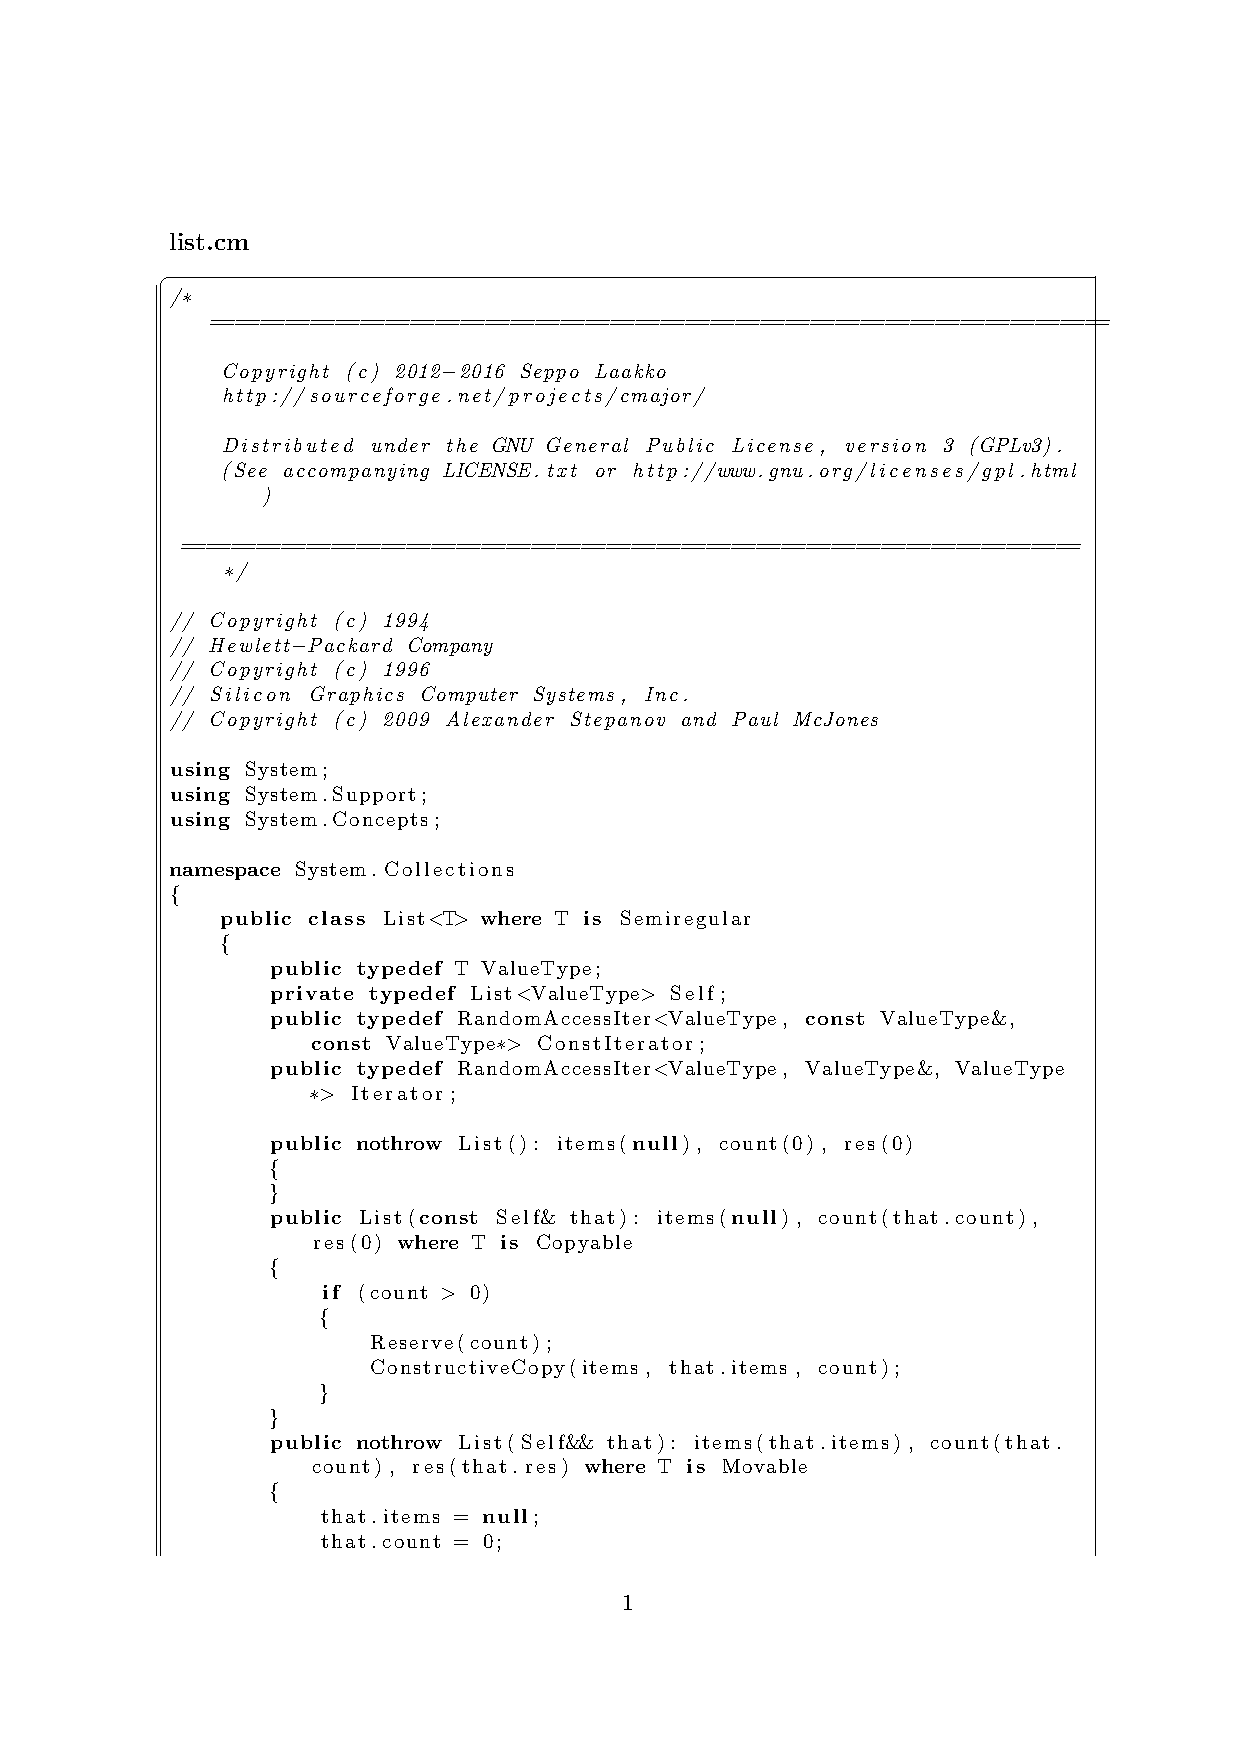
\includegraphics{list}
\end{center}
\end{figure}

\item
A \emph{postfix} expression is denoted by $\theta_i$ in a list expression $\theta_1 (\, \% \, \theta_2)?$
A postfix expression is an expression optionally followed by one of the symbols $*$, $+$, or $?$:

$$\eta ('*' | '+' | '?')?$$

In the previous expression the parentheses and the last $?$ symbol are metasymbols, not terminal symbols.

The postfix expressions containing symbols $*$, $+$, and $?$ are:

\begin{enumerate}
\item
$\eta^*$:
If the input consists of a possibly empty sequence of strings $s_i$ of terminal symbols where each string $s_i$ mathes expression $\eta$,
the input matches expression $\eta^*$. For example, strings $\{\epsilon, \verb|a|, \verb|aa|, \verb|aaa|\}$ match expression $\textbf{a}^*$.

A \emph{closure} node is a unary parsing node whose child subtree represents expression $\eta$.

\item
$\eta^+$:
If the input consists of a nonempty sequence of strings $s_i$ of terminal symbols where each string $s_i$ mathes expression $\eta$,
the input matches expression $\eta^+$. For example, strings $\{\verb|a|, \verb|aa|, \verb|aaa|\}$ match expression $\textbf{a}^+$.

A \emph{positive} node is a unary parsing node whose child subtree represents expression $\eta$.

\item
$\eta?$:
If the input consists either an empty string $\epsilon$, or a string $s$ of terminal symbols where $s$ matches expression $\eta$,
the input matches expression $\eta?$. For example, strings $\{\epsilon, \verb|a|\}$ match expression $\textbf{a}?$.

An \emph{optional} node is a unary parsing node whose child subtree represents expression $\eta$.

\end{enumerate}

Figure \ref{fig:postfix} shows the postfix nodes.

\begin{figure}[htb]
\caption{Postfix Nodes}
\label{fig:postfix}
\vspace{0.5cm}
\begin{center}
\includegraphics{postfix}
\end{center}
\end{figure}

\item
A \emph{primary} expression is denoted by $\eta$ in a postfix expression $\eta ('*' | '+' | '?')?$.

Using extended context-free grammar notation, a primary expression can be expressed as:

$$primary \rightarrow (\> primitive \> | \> nonterminal \> | \> grouping \> | \> token \>) \> expectation? \> action?$$

That is, a primary expression is one of:

\begin{enumerate}
\item
a \emph{primitive} expression, that is an atomic \verb|cmpg| expression.
\item
a \emph{nonterminal} expression that matches input to a rule recursively.
\item
a \emph{grouping} expressions that is a parenthesized alternative expression.
\item
a \emph{token} expression that prevents skipping.
\end{enumerate}

Previous expressions can be optionally followed by an
\emph{expectation} expression that prevents backtracking,
and an \emph{action} expression that associates a semantic action to a primary expression.

\clearpage
\item
The primitive expression is defined using the extended context-free notation as:

\begin{align*}
primitive &\rightarrow \> char |\> string |\> charset |\> keyword |\> keyword\_list \> |\\
&\textbf{empty} |\> \textbf{space} |\> \textbf{anychar} |\> \textbf{letter} |\> \textbf{digit} |\> \textbf{hexdigit} |\> \textbf{punctuation}
\end{align*}

Figure \ref{fig:primitives} shows the primitive expressions, what input they match, and the corresponding node types.

\begin{figure}[htb]
\caption{Primite Expressions}
\label{fig:primitives}
\begin{tabular}{lp{10cm}l}
\textbf{Expression}&\textbf{Matches}&\textbf{Node}\\
\hline
\emph{char}& matches a single terminal symbol to a character specified in the expression. & \framebox[2cm][c]{'x'}\\
\emph{string}& matches a string of terminal symbols to a string specified in the expression. &\framebox[2cm][c]{"abc"}\\
\emph{charset} & matches a single terminal symbol to set of characters specified in the expression. &\framebox[2cm][c]{[abc]}\\
\emph{keyword} & matches a string of terminal symbols to a keyword string specified in the expression. &\framebox[2cm][c]{\textbf{for}}\\
\emph{keyword_list} & matches a string of terminal symbols to a list of keyword strings specified in the expression &\framebox[2cm][c]{\textbf{for,if}}\\
\textbf{empty} & matches always &\framebox[2cm][c]{\textbf{empty}}\\
\textbf{space} & matches a single terminal symbol to any whitespace character&\framebox[2cm][c]{\textbf{space}}\\
\textbf{anychar} & matches a single terminal symbol to any single character&\framebox[2cm][c]{\textbf{anychar}}\\
\textbf{letter} & matches a single terminal symbol to any latin letter&\framebox[2cm][c]{\textbf{letter}}\\
\textbf{digit} & matches a single terminal symbol to any decimal digit&\framebox[2cm][c]{\textbf{digit}}\\
\textbf{hexdigit} & matches a single terminal symbol to any hexadecimal digit&\framebox[2cm][c]{\textbf{hexdigit}}\\
\textbf{punctuation} & matches a single terminal symbol any ASCII punctuation symbol&\framebox[2cm][c]{\textbf{punct}}
\end{tabular}
\end{figure}

\item
A \emph{nonterminal} expression is defined using extended context-free notation as follows:

\begin{align*}
nonterminal &\rightarrow \> (\> identifier \>| \> identifier \> arguments \>) \> alias?\\
arguments &\rightarrow \> '(' argument (\> ',' \> argument\>)^* \> ')'\\
alias &\rightarrow \> ':' \> identifier
\end{align*}

The nonterminal expression names a rule that is matched recursively.
It can contain a parenthesized list of \emph{argument}s, that become the inherited attributes of the ``called'' rule.
We used the word ``called'' because the recursive matching process can be thought as procedures that call each other recursively,
as in recursive-descent parser.

If the called rule has a synthersized attribute and the rule is called many times inside a body of a rule,
the synthesized attribute of the called rule must be given a unique name. That is the use of an \emph{alias} expression.

The node for the nonterminal is represented as $$\framebox[2cm][c]{\emph{nt}(\emph{foo})}$$

where \emph{foo} is the name of the rule matched recursively.

\item
A \emph{grouping} expression is a parenthesized sequence of alternative expressions.

\begin{align*}
grouping &\rightarrow \> '(' \> alternatives \> ')'
\end{align*}

\item
A \emph{token} expression consists of a keyword \textbf{token} followed by a parenthesized sequence of alternative expressions.
It prevents skipping of tokens that match the \emph{skip rule} of the grammar.

\begin{align*}
token &\rightarrow \> \textbf{token} \>'(' \> alternatives \> ')'
\end{align*}

\item
An \emph{expectation} expression is a single '!' symbol associated with the preceding primary expression.
It forces the matching of its preceding expression without backtracking.
If its associated expression does not match, an exception is thrown.

\begin{align*}
expectation &\rightarrow \> '!'
\end{align*}

\item
An \emph{action} expression is a block of C++ code in braces.
It represents a semantic action that is executed if input matches its associated primary expression.

\begin{align*}
action &\rightarrow \> '\{' \> \texttt{C++ code} \> '\}'
\end{align*}

\end{itemize}

Figure \ref{fig:token} shows the token, expectation and action unary parsing nodes.

\begin{figure}[htb]
\caption{Token, Expectation, and Action Nodes}
\label{fig:token}
\vspace{0.5cm}
\begin{center}
\includegraphics{token}
\end{center}
\end{figure}

\clearpage
\begin{exmp} Example of Internal Representation.
\begin{flushleft}
Let us recall the Postfix Translation Grammar of example \ref{ex:postfix}. For ease of reference it is repeated here:

\lstset{language=cmpg}
\begin{lstlisting}
grammar PostfixTranslationGrammar
{
    expr: std::string
        ::= term:t{ value = t; }
        (   '+' term:pt{ value.append(pt).append(1, '+'); }
        |   '-' term:mt{ value.append(mt).append(1, '-'); }
        )*
        ;

    term: std::string
        ::= factor:f{ value = f; }
        (   '*' factor:tf{ value.append(tf).append(1, '*'); }
        |   '/' factor:df{ value.append(df).append(1, '/'); }
        )*
        ;

    factor: std::string
        ::= digit{ value = std::string(1, *matchBegin); }
        |   '(' expr{ value = expr; } ')'
        ;
}
\end{lstlisting}

Figure \ref{fig:parsers} shows the internal representation of the \emph{expr} rule.

\begin{figure}[htb]
\caption{Internal Representation of \emph{expr} Rule}
\label{fig:parsers}
\begin{center}
\includegraphics{parsers}
\end{center}
\end{figure}
\end{flushleft}
\end{exmp}

\clearpage
\subsection{\texttt{cmpg} Language Grammar}

\begin{flushleft}
Here the syntax of the \verb|cmpg| language is presented in extended context-free notation:

\begin{grmr}
\verb|cmpg| Language Grammar.
\begin{align*}
grammar &\rightarrow \> \textbf{grammar} \> identifier \> '\{' \> grammarcontent \> '\}'\\
grammarcontent &\rightarrow \> ( \> startclause \> | \> skipclause \> | \> rulelink \> | \> rule \> )^*\\
startclause &\rightarrow \> \textbf{start} \> identifier \> ';'\\
skipclause &\rightarrow \> \textbf{skip} \> qualifiedid \> ';'\\
rulelink &\rightarrow \> \textbf{using} \> ( \> identifier \> '=' \> qualifiedid \> | \> qualifiedid \> ) \> ';'\\
rule &\rightarrow \> identifier \> locals? \> returns? \> "::=" \> alternatives \> ';'\\
locals &\rightarrow '(' \> (variable \> | \> parameter) \>( \>',' \> (variable \> | \> parameter)) ^* \> ')'\\
variable &\rightarrow \> \textbf{var} \> cpptype \> cppdeclarator\\
parameter &\rightarrow \> cpptype \> cppdeclarator\\
returns &\rightarrow \> ':' cpptype\\
alternatives &\rightarrow catenate \> (\> '|' \> catenate \>)^*\\
catenate &\rightarrow diff^+\\
diff &\rightarrow xor \> ( \> '-' \> xor)^*\\
xor &\rightarrow and \> ( \> \hat{} \> and)^*\\
and &\rightarrow list \> (\> '\&' \> list)^*\\
list &\rightarrow postfix \> (\> '\%' list)?\\
postfix &\rightarrow primary \> ( \> '*' \> | \> '+' \> | \> '?' \>)?\\
primary &\rightarrow (\> primitive \> | \> nonterminal \> | \> grouping \> | \> token \>) \> expectation? \> action?\\
primitive &\rightarrow \> char |\> string |\> charset |\> keyword |\> keyword\_list\\
&| \> \textbf{empty} |\> \textbf{space} |\> \textbf{anychar} |\> \textbf{letter} |\> \textbf{digit} |\> \textbf{hexdigit} |\> \textbf{punctuation}\\
nonterminal &\rightarrow \> (\> identifier \>| \> identifier \> arguments \>) \> alias?\\
arguments &\rightarrow \> '(' argument (\> ',' \> argument\>)^* \> ')'\\
alias &\rightarrow \> ':' \> identifier\\
grouping &\rightarrow \> '(' \> alternatives \> ')'\\
token &\rightarrow \> \textbf{token} \> '(' alternatives \> ')'\\
expectation &\rightarrow \> '!'\\
action &\rightarrow \> '\{' \> \texttt{C++ code} \> '\}'\\
identifier &\rightarrow \> id \> - \> keyword\\
qualifiedid &\rightarrow \> identifier \> ( \> '.' \> identifier)^*\\
id & \rightarrow \> ( \> \textbf{letter} \> | \> '\_' \> ) \> ( \> \textbf{letter} \> | \> \textbf{digit} \> | \> '\_' \> )^*\\
keyword &\rightarrow \> \textbf{using}|\textbf{grammar}|\textbf{start}|\textbf{skip}|\textbf{token}|\textbf{keyword}|\textbf{keyword\_list}\\
&|\textbf{empty}|\textbf{space}|\textbf{anychar}|\textbf{letter}|\textbf{digit}|\textbf{hexdigit}|\textbf{punctuation}|\textbf{var}
\end{align*}
The \emph{cpptype} denotes a \verb|C++| type expression, and the \emph{cppdeclarator} denotes a \verb|C++| declarator.
\end{grmr}
\end{flushleft}

\subsection{Informal Description of Operation of a Parser Generated Using \texttt{cmpg}}

A parser generated using \verb|cmpg| works much the same way than a handwritten recursive-descent parser would operate.
In principle, each rule can be thought as a recursive procedure that receives parameters, or inherited attributes, from its caller, or parent rule,
matches terminals and maybe calls other recursive procedures, or rules, and finally can return a value, a computed synthesized attribute,
to its caller, or parent rule.

The parsing begins by trying to match the start of the input to the body of the rule $S$, the start rule of the grammar.

If the current input position is at the start of rule $P$, and there are many $P$-productions,
$P \rightarrow \omega_1 \,|\, \omega_2 \, | \cdots \, | \, \omega_k$,
the parser tries to match the the input to the production $P \rightarrow \omega_1$.
If the input matches, the other $P$-productions are not tried and the parsing proceeds to the successor of the caller of the production $P \rightarrow \omega_1$.
However, if the input does not match $P \rightarrow \omega_1$, input is backtracked, and the
production $P \rightarrow \omega_2$ is tried, and so on, until either a match is found, or the input did not match the last
$P$-production $P \rightarrow \omega_k$. In that case, let $Q \rightarrow \alpha P \beta \Leftrightarrow Q \rightarrow \upsilon_i$ be the parent of $P$.
At this point the input is backtracked and the next alternative for the caller of the $P$, $Q \rightarrow \upsilon_{i+1}$ is tried.
This process is repeated until either the entire input matches, or a syntax error is detected.

\subsection{Parsing Algorithm}

The algorithm uses a stack of attribute values, a Boolean variable for skipping state $skip$, a stack of skipping states,
and keeps track of \emph{current input position}.
Each rule has a data structure called \emph{context} that contains the current values of inherited attributes,
synthesized attribute, local variables, and synthesized attributes of the contained nonterminals of the rule.
Each rule has also a stack of those context structures called a \emph{context stack}.

When input is parsed using the following algorithm \ref{al:parsing} applied to a parsing node, the result of parsing can be either:

\begin{enumerate}
\item
\textbf{match}(\textbf{true}, \emph{n}), where $n > 0$, to indicate that input matched, and the length of the match was \emph{n} characters.

\item
\textbf{match}(\textbf{true}, 0), to indicate a successful empty match. In this case the current input position was not advanced.

\item
\textbf{match}(\textbf{false}) to indicate that input did not match. In this case we say that the result is a \emph{failure} match.
\end{enumerate}

In the beginning the attribute stack is empty, the skipping state stack is empty, and the skipping state $skip$ is \textbf{true}.
The parsing begins by setting the current input position to the start of the input, and
applying algorithm \ref{al:parsing} to the root node of the parsing node tree that forms
the definition of the start rule of the grammar.
Let $m$ be the result of parsing applied to the root node.

If $m$ is:
\begin{enumerate}
\item
\textbf{match}(\textbf{true}, \emph{n}), where $n$ is the length of the input, the parsing succeeds.
\item
\textbf{match}(\textbf{true}, \emph{n}), where $n$ is less than the length of the input, the parsing fails.
\item
\textbf{match}(\textbf{false}), the parsing fails.
\end{enumerate}

\begin{algo} Parsing Algorithm.\label{al:parsing} (\cite{SPIRIT})

\begin{flushleft}
If the type of the node this algorithm is applied to is:
\begin{enumerate}

\item
Alternative node (Fig. \ref{fig:alternatives}).
Let $save$ be the current input position. Apply this algorithm recursively to the left subtree of this node.
Let $m$ be the result of parsing the left subtree.
\footnote{When we say that a node, or a subtree, is parsed, we mean that input is parsed in the context of that node, or subtree.}
If $m$ was a successful match, let the result of parsing this node be $m$.

Otherwise, backtrack by setting the current input position to \emph{save} and
apply this algorithm recursively to the right subtree of this node.
Let the result of parsing this node be the result of parsing the right subtree.

\item
Catenate node (Fig. \ref{fig:catenate}). Apply this algorithm recursively to the left subtree of this node.
Let $m_1$ be the result of parsing the left subtree.
If $m_1$ a successful match, unless $skip$ is \textbf{false} skip tokens using the skip rule,
then apply this algorithm recursively to the right subtree of this node.
Let $m_2$ be the result of parsing the right subtree.
If $m_2$ was a successful match, let the result of parsing this node be $\textbf{match}(\textbf{true}, length(m_1) + length(m_2))$.

Otherwise, either $m_1$ was a failure match, or $m_2$ was a failure match. Let the result of parsing this node be $\textbf{match}(\textbf{false})$.

\item
Difference node (Fig. \ref{fig:difference}).
Let $save$ be the current input position. Apply this algorithm recursively to the left subtree of this node.
Let $m_1$ be the result of parsing the left subtree.
If $m_1$ was a successful match, let $tmp$ be the current input position, and backtrack by setting the current input position to $save$;
then apply this algorithm recursively to the right subtree of this node. Let $m_2$ be the result of parsing the right subtree.
If $m_2$ was a failure match, or $length(m_2) < length(m_1)$, set the current input position to $tmp$,
and let the result of parsing this node be $m_1$, a successful match.

Otherwise, either $m_1$ was a failure match, or $m_2$ was a successful match with $length(m_2) \ge length(m_1)$.
Let the result of parsing this node be $\textbf{match}(\textbf{false})$.

\item
Xor node (Fig. \ref{fig:xor}). Let $save$ be the current input position. Apply this algorithm recursively to the left subtree of this node.
Let $m_1$ be the result of parsing the left subtree.
Let $tmp$ be the current input position, and backtrack by setting the current input position to $save$.
Apply this algorithm recursively to the right subtree of this node.
Let $m_2$ be the result of parsing the right subtree.
If $m_1$ was a successful match and $m_2$ was a failure match, or $m_1$ was a failure match and $m_2$ was a successful match,
do the following:
\begin{enumerate}
\item
If $m_1$ was a successful match, set the current input position to $tmp$.
\item
If $m_1$ was a successful match, let the result of parsing this node be $m_1$, otherwise let the result of parsing this node be $m_2$.
\end{enumerate}

Otherwise, either both $m_1$ and $m_2$ were successful matches, or both were failure matches.
Let the result of parsing this node be $\textbf{match}(\textbf{false})$.

\item
Intersection node (Fig. \ref{fig:and}).
Let $save$ be the current input position. Apply this algorithm recursively to the left subtree of this node.
Let $m_1$ be the result of parsing the left subtree.
If $m_1$ was a successful match, backtrack by setting the current input position to $save$,
and apply this algorithm recursively to the right subtree of this node.
Let $m_2$ be the be the result of parsing the right subtree.
If $m_2$ was a successful match and $length(m_1) = length(m_2)$, let the result of parsing this node be $m_1$.

Otherwise, either $m_1$ was a failure match, $m_2$ was a failure match, or $length(m_1) \ne length(m_2)$.
Let the result of parsing this node be $\textbf{match}(\textbf{false})$.

\item
List node (Fig. \ref{fig:list}). Apply this algorithm recursively to the child subtree of this node.
Let the result of parsing this node be the result of parsing the child subtree.

\item
Closure node (Fig. \ref{fig:postfix}). Let $m_1$ be $\textbf{match}(\textbf{true},0)$, and let $first$ be \textbf{true}.
Do following in a loop until loop exited:

\begin{enumerate}
\item
Let $save$ be the current input position.
\item
If $first = \textbf{true}$, set $first$ to \textbf{false}, otherwise, unless $skip$ is \textbf{false}, skip tokens using the skip rule.
\item
Apply this algorithm recursively to the child subtree of this node.
Let $m_2$ be the result of parsing the child subtree.
\item
If $m_2$ was a successful match, set $m_1$ to $\textbf{match}(\textbf{true}, length(m_1) + length(m_2))$,
otherwise backtrack by setting the current input position to $save$ and exit the loop.
\end{enumerate}
Let the result of parsing this node be $m_1$.

\item
Positive node (Fig. \ref{fig:postfix}). Apply this algorithm recursively to the child subtree of this node.
Let $m_1$ be the result of parsing the child subtree.

If $m_1$ was a successful match, do following in a loop until loop exited:
\begin{enumerate}
\item
Let $save$ be the current input position.
\item
If $skip$ is \textbf{true}, skip tokens using the skip rule.
\item
Apply this algorithm recursively to the child subtree of this node.
Let $m_2$ be the result of parsing the child subtree.
\item
If $m_2$ was a successful match, set $m_1$ to $\textbf{match}(\textbf{true}, length(m_1) + length(m_2))$,
otherwise backtrack by setting the current input position to $save$ and exit the loop.
\end{enumerate}
Let the result of parsing this node be $m_1$.

\item
Optional node (Fig. \ref{fig:postfix}). Let $save$ be the current input position.
Apply this algorithm recursively to the child subtree of this node.
Let $m$ be the result of parsing the child subtree.
If $m$ was a successful match, let the result of parsing this node be $m$.

Otherwise, backtrack by setting the current input position to $save$.
Let the result of parsing this node be $\textbf{match}(\textbf{true}, 0)$.

\item
Char node (Fig. \ref{fig:primitives}). If current input position is not at the end of the input, and the
character at the current input position is equal to the character contained in this char node,
advance the current input position by one character, and let the result of parsing this node be
$\textbf{match}(\textbf{true}, 1)$.

Otherwise, either the current input position is at the end of the input,
or the character at the current input position is not equal to the character contained in this char node,
so let the result of parsing this node be $\textbf{match}(\textbf{false})$.

\item
String node (Fig. \ref{fig:primitives}). Let $m$ be $\textbf{match}(\textbf{true}, 0)$.
Let $i$ be 0. Let $n$ be the length of the string contained in this string node.

While $i < n$ and the current input position is not at the end of the input and
the character at the current input position is equal to the i'th character of the string contained in this string node,
do the following:
\begin{enumerate}
\item
Advance the current input position by one character.
\item
Increment $i$.
\item
Set $m$ to $\textbf{match}(\textbf{true}, length(m) + 1)$.
\end{enumerate}
If $i = n$, let the result of parsing this node be $m$.

Otherwise let the result of parsing this node be $\textbf{match}(\textbf{false})$.

\item
CharSet node (Fig. \ref{fig:primitives}).
If current input position is not at the end of the input, do the following:
\begin{enumerate}
\item
If the character set is not an inverse set, and the character at the current input position is in the set,
or the character set is an inverse set, and the character at the current input position is not in the set,
advance the current input position by one character,
and let the result of parsing this node be $\textbf{match}(\textbf{true}, 1)$
\end{enumerate}

Otherwise let the result of parsing this node be $\textbf{match}(\textbf{false})$.

\item
Keyword node (Fig. \ref{fig:primitives}). If the contained keyword string is denoted by $k$,
the keyword node contains following expression converted to a tree of parsing nodes:
$k - \textbf{token}(k c)$, where $c$ is usually expression $(\textbf{letter}|\textbf{digit}|'\_'|'.')^+$,
but may also be user supplied \emph{continuation rule}.
Let the result of parsing this node be the result of parsing the contained tree of nodes.

\item
Keyword list node (Fig. \ref{fig:primitives}). The keyword list node has a \emph{selector rule},
that is usually $(\textbf{letter}|'\_')(\textbf{letter}|\textbf{digit}|'\_')^*$,
but may also supplied by the user. The node has also a set of keyword strings $s$.

Let $save$ be the current input position.
First the input is parsed with the selector rule.
Let $m$ be the result of this parsing, and $l$ be the matched lexeme.
If $m$ is a successful match, do the following:
\begin{enumerate}
\item
If the lexeme $l$ matches one of the contained keyword strings $s$,
let the result of parsing this node be $m$,
otherwise backtrack by  setting the current input position to $save$.
\end{enumerate}

Otherwise let the result of parsing this node be $\textbf{match}(\textbf{false})$.

\item
Empty node (Fig. \ref{fig:primitives}). Let the result of parsing this node be $\textbf{match}(\textbf{true}, 0)$.

\item
Space node (Fig. \ref{fig:primitives}). If the current input position is not at the end of the input,
and the character at the current input position is a whitespace character,
advance the current input position by one character,
and let the result of parsing this node be $\textbf{match}(\textbf{true}, 1)$.

Otherwise let the result of parsing this node be $\textbf{match}(\textbf{false})$.

\item
AnyChar node (Fig. \ref{fig:primitives}). If the current input position is not at the end of the input,
advance the current input position by one character,
and let the result of parsing this node be $\textbf{match}(\textbf{true}, 1)$.

Otherwise let the result of parsing this node be $\textbf{match}(\textbf{false})$.

\item
Letter node (Fig. \ref{fig:primitives}). If the current input position is not at the end of the input,
and the character at the current input position is a latin letter character,
advance the current input position by one character,
and let the result of parsing this node be $\textbf{match}(\textbf{true}, 1)$.

Otherwise let the result of parsing this node be $\textbf{match}(\textbf{false})$.

\item
Digit node (Fig. \ref{fig:primitives}). If the current input position is not at the end of the input,
and the character at the current input position is a decimal digit character,
advance the current input position by one character,
and let the result of parsing this node be $\textbf{match}(\textbf{true}, 1)$.

Otherwise let the result of parsing this node be $\textbf{match}(\textbf{false})$.

\item
HexDigit node (Fig. \ref{fig:primitives}). If the current input position is not at the end of the input,
and the character at the current input position is a hexadecimal digit character,
advance the current input position by one character,
and let the result of parsing this node be $\textbf{match}(\textbf{true}, 1)$.

Otherwise let the result of parsing this node be $\textbf{match}(\textbf{false})$.

\item
Punctuation node (Fig. \ref{fig:primitives}). If the current input position is not at the end of the input,
and the character at the current input position is ASCII punctuation character,
advance the current input position by one character,
and let the result of parsing this node be $\textbf{match}(\textbf{true}, 1)$.

Otherwise let the result of parsing this node be $\textbf{match}(\textbf{false})$.

\item
Nonterminal node.
Let the rule that the nonterminal is associated with be $r$.
Parsing proceeds by parsing the rule $r$ recursively as follows:

\begin{enumerate}
\item
Parsing rule $r$ begins by pushing values of arguments specified in this nonterminal node to the attribute stack.
Those arguments will become the inherited attributes of $r$.
Arguments can be current values of inherited attributes, the synthesized attribute,
local variables, or synthesized attributes of the contained nonterminals of the current rule,
i.e. the rule that contains the current nonterminal node.
\item
On entry of parsing the rule $r$, the current context structure of $r$ is pushed
to the context stack of $r$ and the context of $r$ is initialized with default values.
\item
Then arguments are popped off from the attribute stack,
and placed to the context structure of $r$ as inherited attributes.
\item
Apply this algorithm recursively to the root node of the
parsing node tree that forms the definition of the rule $r$.
Let the result of parsing be $m$.
\item
On exit of parsing the rule $r$, if $m$ was a successful match, the value of the synthesized attribute of $r$, if any, is
pushed to the attribute stack. Then in any case, the previous context of $r$ is popped off from
the context stack of $r$, and it becomes the current context of $r$.
\item
If $m$ was a successful match, the synthesized attribute of $r$, if any, is popped off from the attribute stack and
placed to the context structure of the current rule as synthesized attribute of this nonterminal.
\item
Let the result of parsing this node be $m$.
\end{enumerate}

\item
Token node (Fig. \ref{fig:token}). Push the current skipping state $skip$ to the skipping state stack, and set $skip$ to \textbf{false}.
Apply this algorithm recursively to the child subtree of this node.
Let $m$ be the result of parsing the child subtree.
Pop the previous skipping state off from the skipping state stack, and assign it to $skip$.
Let the result of parsing this node be $m$.

\item
Expectation node (Fig. \ref{fig:token}). Apply this algorithm recursively to the child subtree of this node.
Let $m$ be the result of parsing the child subtree.
If $m$ was a failure match, throw \emph{ExpectationFailure} exception, otherwise, let $m$ be the result of parsing this node.

\item
Action node (Fig. \ref{fig:token}). Apply this algorithm recursively to the child subtree of this node.
Let $m$ be the result of parsing the child subtree.
If $m$ was a successful match, do the following:
\begin{enumerate}
\item
Let $matchBegin$ be the start of the matched lexeme and $matchEnd$ be one past the end of the matched lexeme.
Let $pass$ be \textbf{true}.
\item
Call the semantic action associated with this action node by passing pointers $matchBegin$ and $matchEnd$, and reference to $pass$ as arguments.
\item
If the semantic action set $pass$ to \textbf{false}, let the result of parsing this node be $\textbf{match}(\textbf{false})$.
\end{enumerate}
Otherwise, $m$ was a failure match, so if this action has an associated failure action, call it.

In any case, let the result of parsing this node be $m$.
\end{enumerate}

\end{flushleft}

\end{algo}

\clearpage
\subsection{Grammars for Cmajor Language Elements}

Let us take a look at some language elements of Cmajor programming language and
how they are represented using \verb|cmpg| grammars.

\subsubsection{Basic Types}

The grammar for parsing names of basic types is one of the simplest.
It consists of an alternative for each keyword of a basic type.
The semantic action associated with a keyword of the type creates an abstract syntax tree node for it and assigns
it to the synthesized attribute of the rule, that is exposed to semantic actions as an identifier \emph{value}:

\lstset{language=cmpg}
\begin{lstlisting}
grammar BasicTypeGrammar
{
    BasicType: Cm::Ast::Node*
        ::=  keyword("bool"){ value = new Cm::Ast::BoolNode(span); }
        |    keyword("sbyte"){ value = new Cm::Ast::SByteNode(span); }
        |    keyword("byte"){ value = new Cm::Ast::ByteNode(span); }
        |    keyword("short"){ value = new Cm::Ast::ShortNode(span); }
        |    keyword("ushort"){ value = new Cm::Ast::UShortNode(span); }
        |    keyword("int"){ value = new Cm::Ast::IntNode(span); }
        |    keyword("uint"){ value = new Cm::Ast::UIntNode(span); }
        |    keyword("long"){ value = new Cm::Ast::LongNode(span); }
        |    keyword("ulong"){ value = new Cm::Ast::ULongNode(span); }
        |    keyword("float"){ value = new Cm::Ast::FloatNode(span); }
        |    keyword("double"){ value = new Cm::Ast::DoubleNode(span); }
        |    keyword("char"){ value = new Cm::Ast::CharNode(span); }
        |    keyword("wchar"){ value = new Cm::Ast::WCharNode(span); }
        |    keyword("uchar"){ value = new Cm::Ast::UCharNode(span); }
        |    keyword("void"){ value = new Cm::Ast::VoidNode(span); }
        ;
}
\end{lstlisting}

\begin{flushleft}
\emph{span} is a name for a structure exposed to semantic actions that represents a range of input positions.
It contains four integer attributes:
\begin{enumerate}
\item
\emph{fileIndex} is an opaque integer given by user in the main parsing function that identifies the file being parsed.
\item
\emph{lineNumber} is the line number of the matched lexeme counted from the start of the file being parsed.
\item
\emph{start} is the starting position of the matched lexeme.
\item
\emph{end} is the ending position of the matched lexeme.
\end{enumerate}

The start and end positions are measured from the beginning of the whole input string given in the main parsing function.
\end{flushleft}

\subsubsection{Type Expressions}

Next we go through the composition of type expressions.
In the beginning of type expression grammar there are declarations that begin with the keyword \textbf{using}.
They are \emph{rule link}s. A rule link refers to a rule defined in another grammar.
It brings the name of a rule to the scope of the grammar being defined.

\lstset{language=cmpg}
\begin{lstlisting}
grammar TypeExprGrammar
{
    using BasicTypeGrammar.BasicType;
    using IdentifierGrammar.Identifier;
    using IdentifierGrammar.QualifiedId;
    using TemplateGrammar.TemplateId;
    using ExpressionGrammar.Expression;
    ...
\end{lstlisting}

\begin{flushleft}
The \emph{TypeExpr} rule is the start rule of the \emph{TypeExprGrammar} grammar:
\end{flushleft}

\lstset{language=cmpg}
\begin{lstlisting}
    ...
    TypeExpr(
        ParsingContext* ctx,
        var std::unique_ptr<Cm::Ast::DerivedTypeExprNode> node
        ): Cm::Ast::Node*
        ::= empty
        {
            ctx->BeginParsingTypeExpr();
            node.reset(new Cm::Ast::DerivedTypeExprNode(span));
        }
            PrefixTypeExpr(ctx, node.get())
        {
            node->GetSpan().SetEnd(span.End());
            value = Cm::Ast::MakeTypeExprNode(node.release());
            ctx->EndParsingTypeExpr();
        }
        /
        {
            ctx->EndParsingTypeExpr();
        }
    ;
    ...
\end{lstlisting}

\begin{flushleft}
The \emph{TypeExpr} rule has one inherited attribute, \verb|ctx|, of type \verb|ParsingContext*|, and
one local variable, \verb|node|, of type \verb|std::unique_ptr<DerivedTypeExprNode>|.
\end{flushleft}

The body of the rule begins with keyword \textbf{empty} that matches anything without consuming any input.
The semantic action associated with it constructs an abstract syntax tree node \emph{DerivedTypeExprNode},
that eventually becomes the synthesized attribute of this rule, if the rule happens to match.
The reason that the type of \verb|node| is a unique pointer and not an ordinary one is that we don't
want to leak memory in the case that the rule does not match.

The type of the inherited attribute \verb|ctx*|, \emph{ParsingContext}, is a class that is used throughout parsing.
It contains Boolean flags that guide the parsing, stacks of Boolean flags that hold the previous values of those flags,
and member functions for manipulating those flags.

For example, member function \emph{BeginParsingTypeExpr()} pushes the old value of \emph{parsingTypeExpr} flag to the
stack and sets the \emph{parsingTypeExpr} flag to \textbf{true}.
Correspondingly the \emph{EndParsingTypeExpr()} member function pops the previous value of the \emph{parsingTypeExpr} flag off from the
stack and assign it to \emph{parsingTypeExpr}.
The reason that the flags are manipulated using stacks is that parsing is a highly recursive process, and
we may have several instances of the same rule active at one time.
Therefore we must push the old value to the stack when we start parsing a rule, and pop it off when we end parsing that rule.

In line 11 we match the \emph{PrefixTypeExpr} rule recursively.
We pass \verb|ctx| and pointer to \verb|node| as arguments to the \emph{PrefixTypeExpr} rule.
They become inherited attributes of that rule.

The semantic action associated with the \emph{PrefixTypeExpr} nonterminal sets the value of the synthesized attribute of the rule.
If the type expression is a simple one, \emph{value} actually receives the simple type expression node contained by \emph{DerivedTypeExprNode},
otherwise value receives the full \emph{DerivedTypeExprNode}.

The semantic action after the \verb|/| symbol starting line 18 is a \emph{failure action}.
It is executed if matching the rule fails. Thus we call \emph{BeginParsingTypeExpr()} function at the start of the rule,
and \emph{EndParsingTypeExpr()} function at the end of the rule regardless whether matching the rule succeeds or fails.

\begin{flushleft}
The next rule of the \emph{TypeExprGrammar} grammar is the \emph{PrefixTypeExpr} rule:
\end{flushleft}

\lstset{language=cmpg}
\begin{lstlisting}
    ...
    PrefixTypeExpr(
        ParsingContext* ctx, Cm::Ast::DerivedTypeExprNode* node)
        ::= keyword("const"){ node->AddConst(); }
            PostfixTypeExpr(ctx, node):c
        |   PostfixTypeExpr(ctx, node)
        ;
    ...
\end{lstlisting}

\begin{flushleft}
A \emph{prefix} type expression is a \emph{postfix} type expression optionally prefixed by the keyword \textbf{const}.
It has two inherited attributes, a \emph{parsing context} and a pointer to the abstract syntax tree node we are constructing.
\end{flushleft}

\begin{flushleft}
A \emph{postfix} type expression is a \emph{primary} type expression followed by zero or more
\emph{postfix type operators} $., \&\&, \&, *, \textrm{and} [\,]$:
\end{flushleft}

\lstset{language=cmpg}
\begin{lstlisting}
    ...
    PostfixTypeExpr(
        ParsingContext* ctx, Cm::Ast::DerivedTypeExprNode* node,
        var Span s)
        ::= PrimaryTypeExpr(ctx, node){ s = span; }
        (   '.' Identifier!{ ... }
        |   "&&"{ node->AddRvalueRef(); }
        |    '&'{ node->AddReference(); }
        |    '*'{ node->AddPointer(); }
        |   '['{ node->AddArray(); }
            Expression(ctx):dim{ node->AddArrayDimensionNode(dim); }
            ']'
        )*
        ;
    ...
\end{lstlisting}

\begin{flushleft}
A \emph{primary} type expression is either a name of a basic type, i.e. \textbf{bool}, \textbf{sbyte}, etc.,
a template identifier such as \emph{foo}$<$\textbf{int}$>$, a name of a type, $Symbol$ for instance,
or a parenthesized \emph{prefix} type expression.
\end{flushleft}

\lstset{language=cmpg}
\begin{lstlisting}
    ...
    PrimaryTypeExpr(
        ParsingContext* ctx, Cm::Ast::DerivedTypeExprNode* node)
        ::= BasicType{ node->SetBaseTypeExpr(BasicType); }
        |   TemplateId(ctx){ node->SetBaseTypeExpr(TemplateId); }
        |   Identifier{ node->SetBaseTypeExpr(Identifier); }
        |   '('{ node->AddLeftParen(); } PrefixTypeExpr(ctx, node)! ')'{ node->AddRightParen(); }
        ;
}
\end{lstlisting}

\subsubsection{Template Identifiers}

The \emph{template identifier} has one inherited attribute:
\verb|ctx| of type \verb|ParsingContext*|,
and one local variable \verb|templateId| of type
\verb|std::unique_ptr<TemplateIdNode>| that
becomes the value of the inherited attribute of the rule.

\lstset{language=cmpg}
\begin{lstlisting}
grammar TemplateGrammar
{
    using IdentifierGrammar.Identifier;
    using IdentifierGrammar.QualifiedId;
    using TypeExprGrammar.TypeExpr;

    TemplateId(ParsingContext* ctx,
        var std::unique_ptr<TemplateIdNode> templateId): Cm::Ast::Node*
        ::= empty{ ctx->BeginParsingTemplateId(); }
        (
            QualifiedId:subject
            {
                templateId.reset(new TemplateIdNode(span, subject));
            }
            '<'
            (   TypeExpr(ctx):templateArg
                {
                    templateId->AddTemplateArgument(templateArg);
                }
                %
                ','
            )
            '>'
        )
        {
            ctx->EndParsingTemplateId();
            value = templateId.release();
            value->GetSpan().SetEnd(span.End());
        }
        ...
\end{lstlisting}

At the beginning of the rule \emph{BeginParsingTemplateId()}
member function of the \emph{ParsingContext} is called.
Correspondingly at the end of the rule
\emph{EndParsingTemplateId()} member function of the \emph{ParsingContext}
is called regardless whether the parsing succeeds or fails.
\emph{BeginParsingTemplateId()} function pushes the value of member variable
\emph{parsingTemplateId} to the stack and sets \emph{parsingTemplateId} to \textbf{true}.
\emph{EndParsingTemplateId()} function pops the previous value of member variable
\emph{parsingTemplateId} off from the stack and assigns it to
\emph{parsingTemplateId}.

Template identifier consists of a qualified identifier, $foo$, $bar.bazz$, etc.,
followed a list of one or more \emph{type expressions} between
angle brackets. Thus the \emph{TypeExpr} rule
is called recursively by this rule.

\lstset{language=cmpg}
\begin{lstlisting}
        ...
        /
        {
            ctx->EndParsingTemplateId();
        }
    ;
    ...
\end{lstlisting}

\subsubsection{Expressions}

In the beginning of \emph{Expression} grammar there are some rule link declarations.
These are the external rules that this grammar uses:

\lstset{language=cmpg}
\begin{lstlisting}
grammar ExpressionGrammar
{
    using LiteralGrammar.Literal;
    using BasicTypeGrammar.BasicType;
    using IdentifierGrammar.Identifier;
    using IdentifierGrammar.QualifiedId;
    using TemplateGrammar.TemplateId;
    using TypeExprGrammar.TypeExpr;
    ...
\end{lstlisting}

The start rule of the grammar is the \emph{Expression} rule.
It has one inherited attribute \verb|ctx| of type \verb|ParsingContext|.

An \emph{expression} consists of an \emph{equivalence expression}.
The value of \verb|ctx| is passed as an argument to the \emph{Equivalence} rule.
After matching \emph{Equivalence}, the synthesized attribute of the \emph{Expression}
rule is set to the value of the synthesized attribute of the \emph{Equivalence} rule.

\lstset{language=cmpg}
\begin{lstlisting}
    ...
    Expression(ParsingContext* ctx): Cm::Ast::Node*
        ::= Equivalence(ctx){ value = Equivalence; }
        ;
    ...
\end{lstlisting}

An \emph{equivalence} expression consists of a nonempty sequence of \emph{implication}
expressions separated by $<=>$ symbols:
$\alpha_1 <=> \alpha_2 <=> \cdots <=> \alpha_k$.
If $k > 1$ and we are not parsing a concept definition, or we are parsing a template identifier,
we reject the input by setting $pass$ to \textbf{false}.
This is the way to make semantic decisions during parsing.
An expression of the form $\alpha_1 <=> \alpha_2$ is accepted only in a concept definition.
Sole \emph{implication} expression $\alpha_1$ is accepted always.

\lstset{language=cmpg}
\begin{lstlisting}
    ...
    Equivalence(ParsingContext* ctx,
        var std::unique_ptr<Node> expr,
        var Span s): Cm::Ast::Node*
        ::=
        (   Implication(ctx):left{ expr.reset(left); s = span; }
            (   "<=>"
                {
                    if (!ctx->ParsingConcept()
                    || ctx->ParsingTemplateId())
                        pass = false;
                }
                Implication(ctx):right!
                {
                    s.SetEnd(span.End());
                    expr.reset(new EquivalenceNode(s, expr.release(), right));
                }
            )*
        )
        {
            value = expr.release();
        }
        ;
    ...
\end{lstlisting}

An \emph{implication} expression is of the form $\beta_1 (=> \beta_2 (=> \cdots (=> \beta_k)))$
The parentheses show that operands of an implication associate to the right.
We can express such right associative expressions by using \emph{right recursion},
as in the following \emph{Implication} rule:

\lstset{language=cmpg}
\begin{lstlisting}
    ...
    Implication(ParsingContext* ctx, var std::unique_ptr<Node> expr,
        var Span s): Cm::Ast::Node*
        ::=
        (   Disjunction(ctx):left{ expr.reset(left); s = span; }
            (   "=>"
                {
                    if (!ctx->ParsingConcept()
                    || ctx->ParsingTemplateId())
                    pass = false;
                }
                Implication(ctx):right!
                {
                    s.SetEnd(span.End());
                    expr.reset(new ImplicationNode(s, expr.release(), right));
                }
            )?
        )
        {
            value = expr.release();
        }
        ;
    ...
\end{lstlisting}

A right recursive rule is of the form $$p \rightarrow q \> ( \> op \> p \>)?$$ where $op$ is an operator that associates to the right.
Like in \emph{equivalence} expression, the implication expression of the form $\beta_1 => \beta_2$ is also accepted only in concept definitions.
Sole \emph{disjunction} expression $\beta_1$ is accepted always.

The \emph{disjunction } rule rejects meaningless statements like $a || b = c;$, where $a || b$ is an \emph{lvalue}.
That is, when we are parsing the left part of an assignment statement, we set $parsingLvalue$ flag is \textbf{true},
so in that case we reject expression of the form $a || b$.

\lstset{language=cmpg}
\begin{lstlisting}
    ...
    Disjunction(ParsingContext* ctx, var std::unique_ptr<Node> expr,
        var Span s): Cm::Ast::Node*
        ::=
        (   Conjunction(ctx):left{ expr.reset(left); s = span; }
            (   "||"
                {
                    if (ctx->ParsingLvalue()
                    || ctx->ParsingSimpleStatement()
                        && !ctx->ParsingArguments())
                        pass = false;
                }
                Conjunction(ctx):right!
                {
                    s.SetEnd(span.End());
                    expr.reset(new DisjunctionNode(s, expr.release(), right));
                }
            )*
        )
        {
            value = expr.release();
        }
    ;
    ...
\end{lstlisting}

Rules for other expressions are not shown, because there is nothing new in them.
However, we show the syntax of \emph{primary} expression.
A \emph{primary} expression consists one of
\begin{enumerate}
\item
a parenthesized \emph{expression},
\item
a \emph{literal},
\item
a name of a basic type,
\item
a \textbf{sizeof} expression,
\item
a \textbf{cast} expression,
\item
a \textbf{construct} expression,
\item
a \textbf{new} expression,
\item
a \emph{template identifier},
\item
an \emph{identifier},
\item
keyword \textbf{this},
\item
keyword \textbf{base} or a
\item
\textbf{typename} expression.
\end{enumerate}

\lstset{language=cmpg}
\begin{lstlisting}
    Primary(ParsingContext* ctx): Cm::Ast::Node*
        ::= ('(' Expression(ctx) ')'){ value = Expression; }
        |   Literal{ value = Literal; }
        |   BasicType{ value = BasicType; }
        |   SizeOfExpr(ctx){ value = SizeOfExpr; }
        |   CastExpr(ctx){ value = CastExpr; }
        |   ConstructExpr(ctx){ value = ConstructExpr; }
        |   NewExpr(ctx){ value = NewExpr; }
        |   TemplateId(ctx){ value = TemplateId; }
        |   Identifier{ value = Identifier; }
        |   keyword("this"){ value = new ThisNode(span); }
        |   keyword("base"){ value = new BaseNode(span); }
        |   (keyword("typename") '(' Expression(ctx):subject ')')
        {
            value = new TypeNameNode(span, subject);
        }
        ;
\end{lstlisting}

\clearpage
\subsubsection{Statements}

The grammar for statements begins with rule link declarations:

\lstset{language=cmpg}
\begin{lstlisting}
grammar StatementGrammar
{
    using stdlib.identifier;
    using KeywordGrammar.Keyword;
    using ExpressionGrammar.Expression;
    using TypeExprGrammar.TypeExpr;
    using IdentifierGrammar.Identifier;
    using ExpressionGrammar.ArgumentList;
    ...
\end{lstlisting}

Here is the definition of the \emph{Statement} rule.
There are brances for each kind of statement that
Cmajor language contains.

\lstset{language=cmpg}
\begin{lstlisting}
    ...
    Statement(ParsingContext* ctx): Cm::Ast::StatementNode*
        ::= LabeledStatement(ctx){ value = LabeledStatement; }
        |   ControlStatement(ctx){ value = ControlStatement; }
        |   TypedefStatement(ctx){ value = TypedefStatement; }
        |   SimpleStatement(ctx){ value = SimpleStatement; }
        |   AssignmentStatement(ctx){ value = AssignmentStatement; }
        |   ConstructionStatement(ctx){ value = ConstructionStatement; }
        |   DeleteStatement(ctx){ value = DeleteStatement; }
        |   DestroyStatement(ctx){ value = DestroyStatement; }
        |   ThrowStatement(ctx){ value = ThrowStatement; }
        |   TryStatement(ctx){ value = TryStatement; }
        |   AssertStatement(ctx){ value = AssertStatement; }
        |   ConditionalCompilationStatement(ctx)
            {
                value = ConditionalCompilationStatement;
            }
        ;
    ...
\end{lstlisting}

The \emph{SimpleStatement} rule consists of an optional expression.
Thus it is the rule that matches also an empty statement
consisting a sole semicolon.

\lstset{language=cmpg}
\begin{lstlisting}
    ...
    SimpleStatement(ParsingContext* ctx,
        var std::unique_ptr<Node> expr): Cm::Ast::StatementNode*
        ::= (empty{ ctx->PushParsingSimpleStatement(true); }
            (Expression(ctx){ expr.reset(Expression); })? ';')
        {
            ctx->PopParsingSimpleStatement();
            value = new SimpleStatementNode(span, expr.release());
        }
        /
        {
            ctx->PopParsingSimpleStatement();
        }
        ;
    ...
\end{lstlisting}

The \emph{ControlStatement} rule consists of cases for
each kind of control statement.

\lstset{language=cmpg}
\begin{lstlisting}
    ...
    ControlStatement(ParsingContext* ctx): Cm::Ast::StatementNode*
        ::= ReturnStatement(ctx){ value = ReturnStatement; }
        |   ConditionalStatement(ctx){ value = ConditionalStatement; }
        |   SwitchStatement(ctx){ value = SwitchStatement; }
        |   WhileStatement(ctx){ value = WhileStatement; }
        |   DoStatement(ctx){ value = DoStatement; }
        |   RangeForStatement(ctx){ value = RangeForStatement; }
        |   ForStatement(ctx){ value = ForStatement; }
        |   CompoundStatement(ctx){ value = CompoundStatement; }
        |   BreakStatement(ctx){ value = BreakStatement; }
        |   ContinueStatement(ctx){ value = ContinueStatement; }
        |   GotoCaseStatement(ctx){ value = GotoCaseStatement; }
        |   GotoDefaultStatement(ctx){ value = GotoDefaultStatement; }
        |   GotoStatement(ctx){ value = GotoStatement; }
        ;
    ...
\end{lstlisting}

We are showing just the definition of the return statement and
while statement rules.

A return statement consists of keyword \textbf{return} followed by
an optional expression and a semicolon.
The \emph{ReturnStatement} rule constructs an abstract syntax tree node
called \emph{ReturnStatementNode}, that takes the input position and
synhesized attribute of the \emph{Expression} rule as arguments,
and assigns it to the synthesized attribute of the rule.
The exclamation mark after the semicolon disables backtracking.
If the semicolon is missing in input, an \emph{ExpectationFailure} exception
containing exact input position is thrown.

\lstset{language=cmpg}
\begin{lstlisting}
    ...
    ReturnStatement(ParsingContext* ctx): Cm::Ast::StatementNode*
        ::= (keyword("return") Expression(ctx)? ';'!)
        {
            value = new ReturnStatementNode(span, Expression);
        }
        ;
    ...
\end{lstlisting}

A while statement consists of keyword \textbf{while},
a Boolean expression and a statement.
The exclamation marks after the parentheses, and the calls of the expression rule and
statement rule disable backtracking and force matching those constructs.
The \emph{WhileStatement} rule constructs an abstract syntax tree node called
\emph{WhileStatementNode} that takes the synthesized attributes of the
\emph{Expression} and \emph{Statement} rules as arguments, and
assigns it to the synthesized attribute of the rule.

\lstset{language=cmpg}
\begin{lstlisting}
    ...
    WhileStatement(ParsingContext* ctx): Cm::Ast::StatementNode*
        ::= (keyword("while") '('! Expression(ctx)! ')'! Statement(ctx)!)
        {
            value = new WhileStatementNode(span, Expression, Statement);
        }
        ;
    ...
\end{lstlisting}

\subsection{Abstract Syntax Tree Class Hierarchy}

There are three abstract node classes in the abstract syntax tree node class hierarchy:
\emph{Node}, \emph{UnaryNode} and \emph{BinaryNode}.

The \emph{Node} class is the root of the abstract syntax tree node class hierarchy.
The \emph{UnaryNode} class is an abstract syntax tree node that has one child node.
The \emph{BinaryNode} class is an abstract syntax tree node that has two child nodes.

\begin{verbatim}
Node
    UnaryNode
    BinaryNode
\end{verbatim}

\subsubsection{Node Classes for Basic Types}

There is a node class for each basic type:

\begin{verbatim}
Node
    BoolNode
    SByteNode
    ByteNode
    ShortNode
    UShortNode
    IntNode
    UIntNode
    LongNode
    ULongNode
    FloatNode
    DoubleNode
    CharNode
    WCharNode
    UCharNode
    VoidNode
\end{verbatim}

\subsubsection{Literal Node Classes}

There is a node class for each kind of literal:

\begin{verbatim}
Node
    BooleanLiteralNode
    SByteLiteralNode
    ByteLiteralNode
    ShortLiteralNode
    UShortLiteralNode
    IntLiteralNode
    UIntLitralNode
    LongLitralNode
    ULongLiteralNode
    FloatLiteralNode
    DoubleLiterallNode
    CharLiteralNode
    StringLiteralNode
    WStringLiteralNode
    UStringLiteralNode
    NullLiteralNode
\end{verbatim}

\subsubsection{Expression Node Classes}

There is a node class for each kind of Cmajor expression:

\begin{verbatim}
Node
    CastNode
    IsNode
    AsNode
    NewNode
    ConstructNode
    ThisNode
    BaseNode
    UnaryNode
        InvokeNode
        IndexNode
        DotNode
        ArrowNode
        PostfixIncNode
        PostfixDecNode
        DerefNode
        AddOfNode
        NotNode
        UnaryPlusNode
        UnaryMinusNode
        ComplementNode
        PrefixIncNode
        PrefixDecNode
        SizeOfNode
        TypeNameNode
    BinaryNode
        EquivalenceNode
        ImplicationNode
        DisjunctionNode
        ConjunctionNode
        BitOrNode
        BitXorNode
        BitAndNode
        EqualNode
        NotEqualNode
        LessNode
        GreaterNode
        LessOrEqualNode
        GreaterOrEqualNode
        ShiftLeftNode
        ShirtRightNode
        AddNode
        SubNode
        MulNode
        DivNode
        RemNode
\end{verbatim}

\subsubsection{Statement Node Classes}

There is a node class for each kind of Cmajor statement:

\begin{verbatim}
Node
    LabelNode
    CatchNode
    CondCompSymbolNode
    CondCompilationPartNode
    CondCompExprNode
        CondCompNotNode
        CondCompPrimaryNode
        CondCompBinExprNode
            CondCompDisjunctionNode
            CondCompConjunctionNode
    StatementNode
        SimpleStatementNode
        ReturnStatementNode
        ConditionalStatementNode
        SwitchStatementNode
        CaseStatementNode
        DefaultStatementNode
        GotoCaseStatementNode
        GotoDefaultStatementNode
        WhileStatementNode
        DoStatementNode
        ForStatementNode
        RangeForStatementNode
        CompoundStatementNode
        BreakStatementNode
        ContinueStatementNode
        GotoStatementNode
        TypedefStatementNode
        AssignmentStatementNode
        ConstructionStatementNode
        DeleteStatementNode
        DestroyStatementNode
        ThrowStatementNode
        TryStatementNode
        ExitTryStatementNode
        BeginCatchStatementNode
        AssertStatementNode
        CondCompStatementNode
\end{verbatim}

\subsubsection{Concept Node Classes}

Node classes relating to concepts:

\begin{verbatim}
Node
    AxiomStatementNode
    AxiomNode
    ConceptIdNode
    ConceptNode
        SameConceptNode
        DerivedConceptNode
        ConvertibleConceptNode
        ExplicitlyConvertibleConceptNode
        CommonConceptNode
        NonReferenceTypeConceptNode
    ConstraintNode
        WhereConstraintNode
        IsConstraintNode
        MultiParamConstraintNode
        TypeNameConstraintNode
        IntrinsicConstraintNode
            SameConstraintNode
            DerivedConstaraintNode
            ConvertibleConstraintNode
            ExplicitlyConvertibleConstraintNode
            CommonConstraintNode
            NonReferenceTypeConstraintNode
        SignatureConstraintNode
            ConstructorConstraintNode
            DestructorConstraintNode
            MemberFunctionConstraintNode
            FunctionConstraintNode
        BinaryConstraintNode
            DisjunctiveConstraintNode
            ConjunctiveConstraintNode
\end{verbatim}

\clearpage
\subsubsection{Class and Function Node Classes}

Node classes relating to classes and functions:

\begin{verbatim}
Node
    MemberVariableNode
    FunctionGroupIdNode
    FunctionNode
        StaticConstructorNode
        ConstructorNode
        DestructorNode
        MemberFunctionNode
            ConversionFunctionNode
    ClassNode
    InitializerNode
        MemberInitializerNode
        BaseInitializerNode
        ThisInitializerNode
\end{verbatim}

\subsubsection{Other Node Classes}

Other kinds of node classes:

\begin{verbatim}
Node
    CompileUnitNode
    ConstantNode
    DelegateNode
    ClassDeletateNode
    DerivedTypeExprNode
    EnumConstantNode
    EnumTypeNode
    IdentifierNode
    InterfaceNode
    NamespaceNode
    AliasNode
    NamespaceImportNode
    ParameterNode
    TemplateParameterNode
    TemplateIdNode
    TypedefNode
\end{verbatim}

\clearpage
\subsection{Example}

The following example shows the result of parsing a function and constructing an abstract syntax tree for it.

\begin{exmp}
The following Cmajor function is used as example input to the parser:

\lstset{language=Cmajor}
\begin{lstlisting}
public nothrow int StrLen(const char* s)
{
    int len = 0;
    if (s != null)
    {
        while (*s != '\0')
        {
            ++len;
            ++s;
        }
    }
    return len;
}
\end{lstlisting}

The following listing shows the resulting abstract syntax tree for parsing the \emph{StrLen} function:

\begin{verbatim}
FunctionNode
    FunctionGroupIdNode(StrLen)
    ParameterNodeList
        ParameterNode
            DerivedTypeExprNode
                DerivationList
                    Derivation.const
                    Derivation.pointer
                CharNode
            IdentifierNode(s)
    CompoundStatementNode
        ConstructionStatementNode
            IntNode
            IdentifierNode(len)
            SByteLiteralNode(0)
        ConditionalStatementNode
            NotEqualNode
                IdentifierNode(s)
                NullLiteralNode
            CompoundStatementNode
                WhileStatementNode
                    NotEqualNode
                        DerefNode
                            IdentifierNode(s)
                        CharLiteralNode('\0')
                    CompoundStatementNode
                        SimpleStatementNode
                            PrefixIncNode
                                IdentifierNode(len)
                        SimpleStatementNode
                            PrefixIncNode
                                IdentifierNode(s)
        ReturnStatementNode
            IdentifierNode(len)
\end{verbatim}

The parser constructs an abstract syntax tree node called \emph{FunctionNode} for the function.
The FunctionNode contains:
\begin{enumerate}
\item
the name of the function group that the function belongs to: \emph{FunctionGroupIdNode}(StrLen).
\item
nodes for each parameter that the function takes.
Each \emph{ParameterNode} consists of nodes for the type and the name of the parameter.
\item
node for the body of the function: \emph{CompoundStatementNode}.
\end{enumerate}

The body consists of an construction statement, an \textbf{if} statement
and a return statement. The \textbf{if} statement consists of a
\textbf{while} statement that has two simple statements in it.
Each simple statement contains a prefix increment expression.
\end{exmp}

\section{Iterating Through the Abstract Syntax Trees using Visitor Design Pattern}

Many of the following phases of compilation iterate through the abstract syntax trees generated by the parser.
Technically the iteration is done using the \emph{visitor} design pattern.

The visitor design pattern enables creation of several algorithms that operate on a object hierarchy
without touching the object hierarchy. In visitor pattern, each object that is part of the object hierarchy
implements a virtual \emph{Accept} member function that takes a parameter of a class derived from common
\emph{Visitor} class. Accept calls \emph{Visit} member function of a visitor by passing itself as a
parameter to the Visit member function.

\begin{figure}[htb]
\caption{Visitor}
\label{fig:visitor}
\begin{center}
\includegraphics{visitor}
\end{center}
\end{figure}

\lstset{language=C++}
\begin{lstlisting}
class Root
{
public:
    virtual void Accept(Visitor& visitor) = 0;
};

class SomeObject1 : public Root
{
public:
    void Accept(Visitor& visitor) override
    {
        visitor.Visit(*this);
    }
};

class SomeObject2 : public Root
{
public:
    void Accept(Visitor& visitor) override
    {
        visitor.Visit(*this);
    }
};

class Container : public Root
{
public:
    void Accept(Visitor& visitor) override
    {
        o1->Accept(visitor);
        o2->Accept(visitor);
        visitor.Visit(*this);
    }
private:
    SomeObject1* o1;
    SomeObject2* o2;
};

class Visitor
{
public:
    virtual void Visit(SomeObject1& someObject1) {}
    virtual void Visit(SomeObject2& someObject2) {}
    virtual void Visit(Container& container) {}
};
\end{lstlisting}
\clearpage
\lstset{language=C++}
\begin{lstlisting}
class Algorithm1 : public Visitor
{
public:
    void Visit(SomeObject1& someObject1) override
    {
        // algorithm 1 for SomeObject1
    }
    void Visit(SomeObject2& someObject2) override
    {
        // algorithm 1 for SomeObject2
    }
    void Visit(Container& container) override
    {
        // algorithm 1 for Container
    }
};

class Algorithm2 : public Visitor
{
public:
    void Visit(SomeObject1& someObject1) override
    {
        // algorithm 2 for SomeObject1
    }
    void Visit(SomeObject2& someObject2) override
    {
        // algorithm 2 for SomeObject2
    }
    void Visit(Container& container) override
    {
        // algorithm 2 for Container
    }
};

void DoAlgorithm1(Container& c)
{
    Algorithm1 algorithm1;
    c.Accept(algorithm1);
}

void DoAlgorithm2(Container& c)
{
    Algorithm2 algorithm2;
    c.Accept(algorithm2);
}
\end{lstlisting}

\subsection{Visitor Pattern Applied in Cmajor}

In Cmajor the visitor pattern is extended by providing two visiting points for containers.
When starting to visit a container, visitor's \verb|BeginVisit(Container&)| member function is called.
Then the contained elements are visited by calling their \verb|Accept| member functions.
Finally, when ending to visit a container, visitor's \verb|EndVisit(Container&)| member function is called.

\begin{exmp} Visiting a Namespace in Cmajor.
\lstset{language=C++}
\begin{lstlisting}
class NamespaceNode
{
public:
    virtual void Accept(Visitor& visitor)
    {
        visitor.BeginVisit(*this);
        for (Node* node : members)
        {
            node->Accept(visitor);
        }
        visitor.EndVisit(*this);
    }
private:
    std::vector<Node*> members;
};

\end{lstlisting}
\end{exmp}

\chapter{Symbol Table}

The next phase of compilation after parsing is constructing a symbol table.

\section{Symbol Table Structure}

A symbol table consists of a tree of symbols.
There are many kinds of symbols.
Container symbols like class and namespace symbols form the interior nodes of the symbol tree.
Simple kind of symbols like constant and parameter symbols form the leaf nodes of the symbol tree.

\subsection{Symbol Class Hierarchy}

The following listing shows the most important kind of symbols:

\begin{verbatim}
Symbol
    FunctionGroupSymbol
    ConceptGroupSymbol
    ConstantSymbol
    EnumConstantSymbol
    TypedefSymbol
    VariableSymbol
        LocalVariableSymbol
        MemberVariableSymbol
        ParameterSymbol
    ContainerSymbol
        FunctionSymbol
        NamespaceSymbol
        ConceptSymbol
        TypeSymbol
            BasicTypeSymbol
                ...
            ClassTypeSymbol
                TemplateTypeSymbol
            DerivedTypeSymbol
            EnumTypeSymbol
            InterfaceTypeSymbol
\end{verbatim}

\subsection{Properties of Symbols}

We inspect properties of symbols that make possible symbol algorithms.

\subsubsection{Properties Common To All Symbols}

The most important attribute common to each kind of symbol is its name.
Another property common to all symbols is a pointer to the symbol's parent symbol in the symbol table.
The global namespace symbol is the root of the symbol tree.
The name of the global namespace symbol is empty and its parent property is null.
Other symbols have a nonempty name and a nonnull parent property.

With the name and parent properties the \emph{full name} of a symbol can be computed.
The algorithm returns a string that consists of nonempty names of symbols along a path from the global namespace symbol to
the symbol separated by dot characters. Fox example, the full name of the global namespace symbol is an empty string, and
the full name of a class symbol whose name is \texttt{gamma} that is contained by namespace symbol whose name is \texttt{beta} that is
contained by a namespace symbol whose name is \texttt{alpha} that is contained by the global namespace symbol is \texttt{alpha.beta.gamma}.

\begin{algo} Computing the Full Name of a Symbol.
\begin{enumerate}
\item
If the symbol's parent property is not null let \emph{p} be the full name of symbol's parent.
Otherwise let \emph{p} be empty string.

\item
If \emph{p} is empty string, the full name of the symbol is the name of the symbol.
Otherwise the full name of the symbol is \emph{p} concatenated with "." and the name of the symbol.
\end{enumerate}

\end{algo}

With the parent property also an associated namespace symbol for a symbol can be computed as follows:

\begin{algo}\label{associatedns} Computing an Associated Namespace Symbol for a Symbol.
\begin{enumerate}
\item
Let $s$ be the symbol for which to compute the associated namespace symbol.
\item
If $s$ is a namespace symbol, return $s$.
\item
Otherwise, if the parent symbol of $s$ is not null, compute the associated namespace symbol for the parent symbol of $s$
and return it.
\item
Otherwise, throw an exception.
\end{enumerate}
\end{algo}

\subsubsection{Properties of Container Symbols}

Each container symbol, say \emph{S}, like a namespace or a class symbol, has a \emph{container scope}, say \emph{C}, that
keeps a mapping from names of contained symbols to contained symbols themselves.
A container scope \emph{C} also has pointers to its \emph{base scope} and its \emph{parent scope}.
If \emph{S} is a class type symbol, the base scope of \emph{C} is the container scope of the base class symbol of \emph{S}.
The parent scope of \emph{C} is the container scope of the parent symbol of \emph{S}.
A container scope also contains a pointer to its owning container symbol.

\subsection{Symbol Name Lookup}\label{namelookup}

Symbol name lookup searches a symbol from a number of container scopes using a possibly qualified name,
a scope kind, and kinds of a symbols to search.
A scope kind is a combination of following values: \textbf{this}, \textbf{base} and \textbf{parent}.
The kind of symbol to search can be one of many values.
For example, lookup: \textbf{all} symbols, only \textbf{type} symbols, only \textbf{namespace} symbols, only \textbf{variable} and \textbf{parameter} symbols, etc.

Let $c_1$, \ldots, $c_n$ be the components of a qualified name to search. The components are separated by dots.
For example, if the name to search is \texttt{alpha}, then $n = 1$ and $c_1 = \texttt{alpha}$.
Another example: if the name to search is \texttt{alpha.beta}, then $n = 2$, $c_1 = \texttt{alpha}$ and $c_2 = \texttt{beta}$.

\subsubsection{Unqualified Name Lookup}

If $n = 1$, we have a simple name and the symbol name lookup performs an \emph{unqualified name lookup}:

\begin{algo}\label{unqualified} Unqualified Name Lookup.
The algorithm returns a symbol if the search is successful, or null otherwise.
\begin{enumerate}
\item
Let \emph{s} be the name to search, \emph{t} be the container scope from which the search begins,
\emph{p} be the set of scope kinds to search, and \emph{k} be the kind of symbol to search.
\item
If \emph{s} is found from the mapping of \emph{t}, let \emph{m} be the mapped symbol.
If the symbol kind of \emph{m} is equal to \emph{k}, return symbol \emph{m}.
\item
If \emph{p} contains the \textbf{base} scope and the base scope of \emph{t} is not null,
perform unqualified name lookup from the base scope of \emph{t}.
If that search is successful, return the symbol found.
\item
If \emph{p} contains the \textbf{parent} scope and the parent scope of \emph{t} is not null,
perform unqualified name lookup from the parent scope of \emph{t}.
If that search is successful, return the symbol found.
\item
Otherwise, return null.
\end{enumerate}
\end{algo}

\subsubsection{Qualified Name Lookup}

If $n > 1$, we have a qualified name of at least two components and the symbol name lookup performs a
\emph{qualified name lookup}:

\begin{algo} Qualified Name Lookup.
The algorithm returns a symbol if the search is successful, or null otherwise.
\begin{enumerate}
\item
Let $c_1$, \ldots, $c_n$ be the components of a qualified name to search ($n > 1$),
\emph{t} and \emph{u} be the container scope from which the search begins,
\emph{p} be the set of scope kinds to search, and \emph{k} be the kind of symbol to search,
flag \emph{a} be \textbf{true},
symbol \emph{s} be null.
\item
For $i$ = 1, \dots, $n$:
\begin{enumerate}
\item
If $t$ is not null, perform unqualified name lookup (algorithm \ref{unqualified}) for name $c_i$, using scope $t$ and scope kind \textbf{this}.
If $i < n$, set the kind of symbol to search to only \textbf{container} symbols, otherwise, if $i = n$, set the kind of symbol to search to $k$.
If the search was successful, let $s$ be the returned symbol, and let $t$ be the container scope of $s$.
Otherwise let $t$ be null and let $a$ be \textbf{false}.
\end{enumerate}
\item
If $s$ is null or $a$ is \textbf{false}, and if \textbf{parent} scope is in $p$ and the parent scope of $u$ is not null,
perform qualified name lookup (this algorithm) for the parent scope of $u$.
If the search was successful, return the symbol found. Otherwise return null.
\item
Otherwise return symbol $s$.
\end{enumerate}
\end{algo}

\subsection{Opening and Closing Container Symbols}\label{opencontainersymbol}

A symbol table also keeps track of \emph{currently open container symbol} and a \emph{stack of open container symbols}.
Initially the currently open container symbol is the global namespace symbol (the root of the symbol tree), and the
stack of open container symbols is empty.

A nonnamespace container symbol is opened by pushing the currently open container symbol to the stack of open container symbols,
and then setting the container symbol as the currently open container symbol.
Any container symbol is closed by popping a container symbol from the stack of open container symbols and setting it
as the currently open container symbol.

\subsubsection{Opening a Namespace}

A namespace is opened using the following algorithm:

\begin{algo}\label{openns} Opening a Namespace. The algorithm sets the currently open container symbol of a symbol table.
\begin{enumerate}
\item
Let $n$ be a possibly qualified namespace name to open. Let $t$ be a symbol table to which to open the namespace.
\item
If $n$ is an empty string, push the currently open container symbol to the stack of open container symbols of $t$,
and then set the global namespace symbol as the currently open container symbol of $t$.
\item
Otherwise lookup $n$ (see section \ref{namelookup}) from the container scope of the currently open container symbol using scope kind \textbf{this} and
setting the kind of symbols to search as \textbf{namespace} symbols. If the search was successful, let $s$ be the symbol found,
otherwise let $s$ be null.
\item
If $s$ is a namespace symbol, push the currently open container symbol to the stack of open container symbols of $t$,
and then set $s$ as the currently open container symbol of $t$. Otherwise if $s$ is not a namespace symbol, throw an exception.
\item
Otherwise $s$ is null, so use algorithm \ref{createns} to create a namespace to the container scope of the currently open container symbol of $t$,
and open it by pushing the currently open container symbol to the stack of open container symbols of $t$,
and then set the created namespace symbol as the currently open container symbol of $t$.
\end{enumerate}
\end{algo}

\clearpage
\subsubsection{Creating a Namespace}

A namespace is created using the following algorithm:

\begin{algo}\label{createns} Creating a Namespace. The algorithm returns created namespace symbol.
\begin{enumerate}
\item
Let $m$ be a possibly qualified namespace name to create and let $t$ be the container scope to which the namespace symbol is to be created.
Let $c_1$, \ldots, $c_n$ be the $n$ components of $m$ separated by dots.
Let $p$ be the namespace symbol associated with the owner symbol of the container scope $t$.
It can be computed using algorithm \ref{associatedns}.
\item
For $i$ = 1, \ldots, $n$:
\begin{enumerate}
\item
Lookup name $c_i$ (see section \ref{namelookup})
from container scope $t$ using scope kind \textbf{this} and setting the kind of symbols to search as \textbf{namespace} symbols.
If the search was successful let $s$ be the symbol found. Otherwise let $s$ be null.
\item
If $s$ is not null and $s$ is a namespace symbol, let $t$ be the container scope of $s$ and
let $p$ be the namespace symbol associated with the owner symbol of the container scope $t$ (algorithm \ref{associatedns}).
Otherwise if $s$ is not null and $s$ is not a namespace symbol, throw an exception.
\item
Otherwise $s$ is null, so create a new namespace symbol $ns$ with name $c_i$. Let $t$ be the container scope of $ns$.
Let the parent scope of $t$ be the container scope of $p$. Add symbol $ns$ as the child symbol of $p$. Finally let $p$ be $ns$.
\end{enumerate}
\item
Return $p$.
\end{enumerate}
\end{algo}

\subsection{Adding Symbols to Containers}

A symbol is added as a child of a container symbol using the following algorithm:

\begin{algo}\label{addsymboltocontainer} Adding a Symbol to a Container.
\begin{enumerate}
\item
Let $s$ be the symbol to add to a container symbol $c$.
\item
If the name of $s$ is not empty and $s$ is not a function symbol and $s$ is not a concept symblol and $s$ is not a declaration block symbol and
$s$ is not a namespace type symbol, install the symbol to the container scope of $c$ using following steps:
\begin{enumerate}
\item
If the name of $s$ is found from symbol name mappings of the container scope of $c$, throw an exception,
because the name of a symbol must be unique in its immediate container.
\item
Add a mapping from name of $s$ to $s$ to the $name \rightarrow symbol$ mapping of the container scope of $c$.
\item
If symbol is a container symbol, set the parent scope of the container scope of $s$ to the container scope of $c$.
\end{enumerate}
\item
If $s$ if a function symbol, open a function group using the group name of $s$ and add $s$ to the opened function group using algorithm
\ref{addtofunctiongroup}.
\item
Otherwise, if $s$ is a concept symbol, open a concept group using the group name of $s$ and add $s$ to the opened concept group using algorithm
\ref{addtoconceptgroup}.
\item
Othwerwise, add $s$ as a child symbol of $c$ and set the parent property of $s$ to $c$.
\end{enumerate}
\end{algo}

\subsubsection{Function Groups}

Function symbols are not added directly to containers, but there is an extra layer called a \emph{function group}
in between the container symbol and the function symbol. To describe function groups we need two definitions:

\begin{defn} The \emph{group name} of a nonmember function is the name of the function without its parameters.
The group name of a constructor is "@constructor" and the group name a destructor is "@destructor".
The group name of other member function is the name of the member function without its parameters.
For example, the group name of function
\begin{verbatim}
void foo(int x, double y)
\end{verbatim}
is \verb|foo| and the group name of member function
\begin{verbatim}
void C.operator=(const C& x)
\end{verbatim}
is \verb|operator=|.
\end{defn}

\begin{defn} The \emph{arity} of a function is the number of its parameters.
For example, the arity of function
\begin{verbatim}
void foo(int x, double y)
\end{verbatim}
is 2.
\end{defn}

A function group collects functions that have equal group name under a name.
A function group has a mapping from arities of functions to lists of function symbols.

\begin{exmp}
For example, if we have three functions:
\begin{verbatim}
void foo(int a);
void foo(double b);
void foo(int a, double b);
\end{verbatim}

they all belong to a function group named \emph{foo}.
The function group \emph{foo} contains a mapping from arity 1 to a list containing two functions:
\verb|void foo(int a)| and \verb|void foo(double b)|.
It also contains a mapping from arity 2 to a list containing one function:
\verb|void foo(int a, double b)|.
\end{exmp}

Opening a function group and adding a function to it is performed using the following algorithm:

\begin{algo}\label{addtofunctiongroup} Opening a Function Group, and Adding a Function to it.
\begin{enumerate}
\item
Let $s$ be a function symbol to add to a function group under container $c$.
\item
Lookup the group name of $s$ from the container scope of $c$ using scope kind \textbf{this} (algorithm \ref{unqualified}).
If the search was successful, let $g$ be symbol found. Otherwise let $g$ be null.
\item
If $g$ is null, create a new function group symbol using group name of $s$, and add it to $c$ using
algorithm \ref{addsymboltocontainer}. Let $g$ be the created function group.
\item
Otherwise, if $g$ is not a function group symbol, throw an exception, because name of a function group
conflicts with name of another symbol.
\item
Let $a$ be the arity of $s$. Add the $s$ to a list of functions of arity $a$ in the $arity \rightarrow list$ mappings of $g$.
\item
Add $s$ as a child symbol of $g$.
\end{enumerate}
\end{algo}

\subsubsection{Concept Groups}

What is said about functions and function groups applies analogically to concepts and concept groups.
Concept group acts as a layer between a container and a concept symbol.
Also analogically to a group name and arity of a function, we can define the group name and arity of
a concept as follows:

\begin{defn} The \emph{group name} of a concept is the name of a concept without its type parameters.
For example, the group name of concept
\begin{verbatim}
EqualityComparable<T, U>
\end{verbatim}
is \verb|EqualityComparable|.
\end{defn}

\begin{defn} The \emph{arity} of a concept is the number of its type parameters.
For example, the arity of concept
\begin{verbatim}
EqualityComparable<T, U>
\end{verbatim}
is 2.
\end{defn}

A concept group collects concepts that have equal group name under a name.
A concept group has a mapping from arities of concepts to concept symbols.

\begin{exmp}
For example, if we have these two concepts:
\begin{verbatim}
EqualityComparable<T>
EqualityComparable<T, U>
\end{verbatim}

they both belong to a concept group named \emph{EqualityComparable}.
The concept group \emph{EqualityComparable} contains a mapping from arity 1 to a concept symbol
\verb|EqualityComparable<T>| and from arity 2 to a concept symbol \verb|EqualityComparable<T, U>|.
\end{exmp}

Opening a concept group and adding a concept to it is performed using the following algorithm:

\begin{algo}\label{addtoconceptgroup} Opening a Concept Group, and Adding a Concept to it.
\begin{enumerate}
\item
Let $s$ be a concept symbol to add to a concept group under container $c$.
\item
Lookup the group name of $s$ from the container scope of $c$ using scope kind \textbf{this} (algorithm \ref{unqualified}).
If the search was successful, let $g$ be symbol found. Otherwise let $g$ be null.
\item
If $g$ is null, create a new concept group symbol using group name of $s$, and add it to $c$ using
algorithm \ref{addsymboltocontainer}. Let $g$ be the created concept group.
\item
Otherwise, if $g$ is not a concept group symbol, throw an exception, because name of a concept group
conflicts with name of another symbol.
\item
Let $a$ be the arity of $s$. Set $s$ as a concept for arity $a$ in the $arity \rightarrow concept$ mappings of $g$.
\item
Add $s$ as a child symbol of $g$.
\end{enumerate}
\end{algo}

\section{Construction of the Global Symbol Table}

The global symbol table is built in three stages:

\begin{enumerate}
\item
First basic type symbols like \emph{BoolTypeSymbol} and \emph{IntTypeSymbol}, and functions that operate on them,
are inserted to the global namespace of the global symbol table.

\item
Then the symbol tables of the referenced libraries are read and imported to the global symbol table.

\item
Finally the abstract syntax trees of the project being compiled are iterated
and symbols that correspond abstract syntax tree nodes are created and inserted to the global symbol table.
\end{enumerate}

\subsection{Insertion of Basic Types and Their Operations}

The first stage in constructing the global symbol table is inserting the basic types and their operations to the global symbol table.
The following listing shows the basic type symbols that are inserted to the global namespace of the global symbol table:

\begin{verbatim}
BasicTypeSymbol
    BoolTypeSymbol
    CharTypeSymbol
    WCharTypeSymbol
    UCharTypeSymbol
    VoidTypeSymbol
    SByteTypeSymbol
    ByteTypeSymbol
    ShortTypeSymbol
    UShortTypeSymbol
    IntTypeSymbol
    UIntTypeSymbol
    LongTypeSymbol
    ULongTypeSymbol
    FloatTypeSymbol
    DoubleTypeSymbol
    NullPtrTypeSymbol
\end{verbatim}

The following listing shows operations for basic types that are inserted to the global namespace of the global symbol table:
\footnote{The group name of the function symbol is shown in brackets after the operation.}

\begin{verbatim}
Symbol
    ContainerSymbol
        FunctionSymbol
            BasicTypeOp
                DefaultCtor[@constructor]
                CopyCtor[@constructor]
                CopyAssignment[operator=]
                MoveCtor[@constructor]
                MoveAssignment[operator=]
                OpEqual[operator==]
                OpLess[operator<]
                BinOp
                    OpAdd[operator+]
                    OpSub[operator-]
                    OpMul[operator*]
                    OpDiv[operator/]
                    OpRem[operator%]
                    OpShl[operator<<]
                    OpShr[operator>>]
                    OpBitAnd[operator&]
                    OpBitOr[operator|]
                    OpBitXor[operator^]
                OpNot[operator!]
                OpUnaryPlus[operator+]
                OpUnaryMinus[operator-]
                OpComplement[operator~]
                OpIncrement[operator++]
                OpDecrement[operator--]
                ConvertingCtor[@constructor]
\end{verbatim}

\subsubsection{Operations for \textbf{bool}}

Operations for \emph{BoolTypeSymbol} are: \emph{DefaultCtor}, \emph{CopyCtor}, \emph{CopyAssignment}, \emph{MoveCtor}, \emph{MoveAssignment},
\emph{OpEqual}, \emph{OpLess}, \emph{OpNot}.

\subsubsection{Operations for Integer Types}

Operations for integer types (\emph{SByteTypeSymbol}, \emph{ByteTypeSymbol}, \emph{ShortTypeSymbol}, \emph{UShortTypeSymbol}, \emph{IntTypeSymbol},
\emph{UIntTypeSymbol}, \emph{LongTypeSymbol}, \emph{ULongTypeSymbol}) are:
\emph{DefaultCtor}, \emph{CopyCtor}, \emph{CopyAssignment}, \emph{MoveCtor}, \emph{MoveAssignment}, \emph{OpEqual}, \emph{OpLess},
\emph{OpAdd}, \emph{OpSub}, \emph{OpMul}, \emph{OpDiv}, \emph{OpRem}, \emph{OpShl}, \emph{OpShr}, \emph{OpBitAnd}, \emph{OpBitOr}, \emph{OpBitXor},
\emph{OpUnaryPlus}, \emph{OpUnaryMinus}, \emph{OpComplement}, \emph{OpIncrement}, \emph{OpDecrement}.

\subsubsection{Operations for Floating Point Types}

Operations for floating point types (\emph{FloatTypeSymbol} and \emph{DoubleTypeSymbol}) are:
\emph{DefaultCtor}, \emph{CopyCtor}, \emph{CopyAssignment}, \emph{MoveCtor}, \emph{MoveAssignment}, \emph{OpEqual}, \emph{OpLess},
\emph{OpAdd}, \emph{OpSub}, \emph{OpMul}, \emph{OpDiv}, \emph{OpUnaryPlus}, \emph{OpUnaryMinus}.

\subsubsection{Operations for Character Types}

Operations for character types (\emph{CharTypeSymbol}, \emph{WCharTypeSymbol} and \emph{UCharTypeSymbol}) are:
\emph{DefaultCtor}, \emph{CopyCtor}, \emph{CopyAssignment}, \emph{MoveCtor}, \emph{MoveAssignment}, \emph{OpEqual}, \emph{OpLess}.

\subsubsection{Standard Conversions}

The following table shows standard conversion operations (\emph{ConvertingCtor})
that are inserted to the global namespace of the global symbol table.

\begin{flushleft}
Abbreviations are:\\
I - implicit conversion,\\
E - explicit conversion,\\
C - conversion,\\
P - promotion
\end{flushleft}

\begin{flushleft}
\begin{supertabular}{lllll}
\textbf{Target Type}& \textbf{Source Type}& \textbf{Explicit/Implicit}& \textbf{Rank}& \textbf{Distance}\\
\hline
\textbf{sbyte}& \textbf{byte}& E& C&\\
\textbf{sbyte}& \textbf{short}& E& C&\\
\textbf{sbyte}& \textbf{ushort}& E& C&\\
\textbf{sbyte}& \textbf{int}& E& C&\\
\textbf{sbyte}& \textbf{uint}& E& C&\\
\textbf{sbyte}& \textbf{long}& E& C&\\
\textbf{sbyte}& \textbf{ulong}& E& C&\\
\textbf{sbyte}& \textbf{float}& E& C&\\
\textbf{sbyte}& \textbf{double}& E& C&\\
\textbf{sbyte}& \textbf{char}& E& C&\\
\textbf{sbyte}& \textbf{wchar}& E& C&\\
\textbf{sbyte}& \textbf{uchar}& E& C&\\
\textbf{sbyte}& \textbf{bool}& E& C&\\
\hline
\textbf{byte}& \textbf{sbyte}& E& C&\\
\textbf{byte}& \textbf{short}& E& C&\\
\textbf{byte}& \textbf{ushort}& E& C&\\
\textbf{byte}& \textbf{int}& E& C&\\
\textbf{byte}& \textbf{uint}& E& C&\\
\textbf{byte}& \textbf{long}& E& C&\\
\textbf{byte}& \textbf{ulong}& E& C&\\
\textbf{byte}& \textbf{float}& E& C&\\
\textbf{byte}& \textbf{double}& E& C&\\
\textbf{byte}& \textbf{char}& E& C&\\
\textbf{byte}& \textbf{wchar}& E& C&\\
\textbf{byte}& \textbf{uchar}& E& C&\\
\textbf{byte}& \textbf{bool}& E& C&\\
\hline
\textbf{short}& \textbf{sbyte}& I& P&1\\
\textbf{short}& \textbf{byte}& I& P&2\\
\textbf{short}& \textbf{ushort}& E& C&\\
\textbf{short}& \textbf{int}& E& C&\\
\textbf{short}& \textbf{uint}& E& C&\\
\textbf{short}& \textbf{long}& E& C&\\
\textbf{short}& \textbf{ulong}& E& C&\\
\textbf{short}& \textbf{float}& E& C&\\
\textbf{short}& \textbf{double}& E& C&\\
\textbf{short}& \textbf{char}& E& C&\\
\textbf{short}& \textbf{wchar}& E& C&\\
\textbf{short}& \textbf{uchar}& E& C&\\
\textbf{short}& \textbf{bool}& E& C&\\
\hline
\textbf{ushort}& \textbf{sbyte}& E& C&\\
\textbf{ushort}& \textbf{byte}& I& P&1\\
\textbf{ushort}& \textbf{short}& E& C&\\
\textbf{ushort}& \textbf{int}& E& C&\\
\textbf{ushort}& \textbf{uint}& E& C&\\
\textbf{ushort}& \textbf{long}& E& C&\\
\textbf{ushort}& \textbf{ulong}& E& C&\\
\textbf{ushort}& \textbf{float}& E& C&\\
\textbf{ushort}& \textbf{double}& E& C&\\
\textbf{ushort}& \textbf{char}& E& C&\\
\textbf{ushort}& \textbf{wchar}& E& C&\\
\textbf{ushort}& \textbf{uchar}& E& C&\\
\textbf{ushort}& \textbf{bool}& E& C&\\
\hline
\textbf{int}& \textbf{sbyte}& I& P&3\\
\textbf{int}& \textbf{byte}& I& P&4\\
\textbf{int}& \textbf{short}& I& P&1\\
\textbf{int}& \textbf{ushort}& I& P&2\\
\textbf{int}& \textbf{uint}& E& C&\\
\textbf{int}& \textbf{long}& E& C&\\
\textbf{int}& \textbf{ulong}& E& C&\\
\textbf{int}& \textbf{float}& E& C&\\
\textbf{int}& \textbf{double}& E& C&\\
\textbf{int}& \textbf{char}& E& C&\\
\textbf{int}& \textbf{wchar}& E& C&\\
\textbf{int}& \textbf{uchar}& E& C&\\
\textbf{int}& \textbf{bool}& E& C&\\
\hline
\textbf{uint}& \textbf{sbyte}& E& C&\\
\textbf{uint}& \textbf{byte}& I& P&2\\
\textbf{uint}& \textbf{short}& E& C&\\
\textbf{uint}& \textbf{ushort}& I& P&1\\
\textbf{uint}& \textbf{int}& E& C&\\
\textbf{uint}& \textbf{long}& E& C&\\
\textbf{uint}& \textbf{ulong}& E& C&\\
\textbf{uint}& \textbf{float}& E& C&\\
\textbf{uint}& \textbf{double}& E& C&\\
\textbf{uint}& \textbf{char}& E& C&\\
\textbf{uint}& \textbf{wchar}& E& C&\\
\textbf{uint}& \textbf{uchar}& E& C&\\
\textbf{uint}& \textbf{bool}& E& C&\\
\hline
\textbf{long}& \textbf{sbyte}& I& P&5\\
\textbf{long}& \textbf{byte}& I& P&6\\
\textbf{long}& \textbf{short}& I& P&3\\
\textbf{long}& \textbf{ushort}& I& P&4\\
\textbf{long}& \textbf{int}& I& P&1\\
\textbf{long}& \textbf{uint}& I& P&2\\
\textbf{long}& \textbf{ulong}& E& C&\\
\textbf{long}& \textbf{float}& E& C&\\
\textbf{long}& \textbf{double}& E& C&\\
\textbf{long}& \textbf{char}& E& C&\\
\textbf{long}& \textbf{wchar}& E& C&\\
\textbf{long}& \textbf{uchar}& E& C&\\
\textbf{long}& \textbf{bool}& E& C&\\
\hline
\textbf{ulong}& \textbf{sbyte}& E& C&\\
\textbf{ulong}& \textbf{byte}& I& P&3\\
\textbf{ulong}& \textbf{short}& E& C&\\
\textbf{ulong}& \textbf{ushort}& I& P&2\\
\textbf{ulong}& \textbf{int}& E& C&\\
\textbf{ulong}& \textbf{uint}& I& P&1\\
\textbf{ulong}& \textbf{long}& E& C&\\
\textbf{ulong}& \textbf{float}& E& C&\\
\textbf{ulong}& \textbf{double}& E& C&\\
\textbf{ulong}& \textbf{char}& E& C&\\
\textbf{ulong}& \textbf{wchar}& E& C&\\
\textbf{ulong}& \textbf{uchar}& E& C&\\
\textbf{ulong}& \textbf{bool}& E& C&\\
\hline
\textbf{float}& \textbf{sbyte}& I& C&5\\
\textbf{float}& \textbf{byte}& I& C&6\\
\textbf{float}& \textbf{short}& I& C&3\\
\textbf{float}& \textbf{ushort}& I& C&4\\
\textbf{float}& \textbf{int}& I& C&1\\
\textbf{float}& \textbf{uint}& I& C&2\\
\textbf{float}& \textbf{long}& E& C&\\
\textbf{float}& \textbf{ulong}& E& C&\\
\textbf{float}& \textbf{double}& E& C&\\
\textbf{float}& \textbf{char}& E& C&\\
\textbf{float}& \textbf{wchar}& E& C&\\
\textbf{float}& \textbf{uchar}& E& C&\\
\textbf{float}& \textbf{bool}& E& C&\\
\hline
\textbf{double}& \textbf{sbyte}& I& C&8\\
\textbf{double}& \textbf{byte}& I& C&9\\
\textbf{double}& \textbf{short}& I& C&6\\
\textbf{double}& \textbf{ushort}& I& C&7\\
\textbf{double}& \textbf{int}& I& C&4\\
\textbf{double}& \textbf{uint}& I& C&5\\
\textbf{double}& \textbf{long}& I& C&2\\
\textbf{double}& \textbf{ulong}& I& C&3\\
\textbf{double}& \textbf{float}& I& P&1\\
\textbf{double}& \textbf{char}& E& C&\\
\textbf{double}& \textbf{wchar}& E& C&\\
\textbf{double}& \textbf{uchar}& E& C&\\
\textbf{double}& \textbf{bool}& E& C&\\
\hline
\textbf{char}& \textbf{sbyte}& E& C&\\
\textbf{char}& \textbf{byte}& E& C&\\
\textbf{char}& \textbf{short}& E& C&\\
\textbf{char}& \textbf{ushort}& E& C&\\
\textbf{char}& \textbf{int}& E& C&\\
\textbf{char}& \textbf{uint}& E& C&\\
\textbf{char}& \textbf{long}& E& C&\\
\textbf{char}& \textbf{ulong}& E& C&\\
\textbf{char}& \textbf{float}& E& C&\\
\textbf{char}& \textbf{double}& E& C&\\
\textbf{char}& \textbf{wchar}& E& C&\\
\textbf{char}& \textbf{uchar}& E& C&\\
\textbf{char}& \textbf{bool}& E& C&\\
\hline
\textbf{wchar}& \textbf{sbyte}& E& C&\\
\textbf{wchar}& \textbf{byte}& E& C&\\
\textbf{wchar}& \textbf{short}& E& C&\\
\textbf{wchar}& \textbf{ushort}& E& C&\\
\textbf{wchar}& \textbf{int}& E& C&\\
\textbf{wchar}& \textbf{uint}& E& C&\\
\textbf{wchar}& \textbf{long}& E& C&\\
\textbf{wchar}& \textbf{ulong}& E& C&\\
\textbf{wchar}& \textbf{float}& E& C&\\
\textbf{wchar}& \textbf{double}& E& C&\\
\textbf{wchar}& \textbf{char}& I& P&1\\
\textbf{wchar}& \textbf{uchar}& E& C&\\
\textbf{wchar}& \textbf{bool}& E& C&\\
\hline
\textbf{uchar}& \textbf{sbyte}& E& C&\\
\textbf{uchar}& \textbf{byte}& E& C&\\
\textbf{uchar}& \textbf{short}& E& C&\\
\textbf{uchar}& \textbf{ushort}& E& C&\\
\textbf{uchar}& \textbf{int}& E& C&\\
\textbf{uchar}& \textbf{uint}& E& C&\\
\textbf{uchar}& \textbf{long}& E& C&\\
\textbf{uchar}& \textbf{ulong}& E& C&\\
\textbf{uchar}& \textbf{float}& E& C&\\
\textbf{uchar}& \textbf{double}& E& C&\\
\textbf{uchar}& \textbf{char}& I& P&2\\
\textbf{uchar}& \textbf{wchar}& I& P&1\\
\textbf{uchar}& \textbf{bool}& E& C&\\
\hline
\textbf{bool}& \textbf{sbyte}& E& C&\\
\textbf{bool}& \textbf{byte}& E& C&\\
\textbf{bool}& \textbf{short}& E& C&\\
\textbf{bool}& \textbf{ushort}& E& C&\\
\textbf{bool}& \textbf{int}& E& C&\\
\textbf{bool}& \textbf{uint}& E& C&\\
\textbf{bool}& \textbf{long}& E& C&\\
\textbf{bool}& \textbf{ulong}& E& C&\\
\textbf{bool}& \textbf{float}& E& C&\\
\textbf{bool}& \textbf{double}& E& C&\\
\textbf{bool}& \textbf{char}& E& C&\\
\textbf{bool}& \textbf{wchar}& E& C&\\
\textbf{bool}& \textbf{uchar}& E& C&\\
\hline
\end{supertabular}
\end{flushleft}

\subsection{Importing Symbol Tables of Referenced Libraries}

The second stage in constructing the global symbol table is
reading the symbol table of referenced libraries and importing the symbols from them into the global symbol table.
For each library L that the project being compiled references,

\begin{itemize}
\item
the symbol table $u$ of L is read from the library file of L and then
\item
the symbols from the global namespace of symbol table $u$ are imported into the global symbol table using algorithm \ref{importns}.
\end{itemize}

\begin{algo}\label{importns} Importing Symbols from a Namespace into a Symbol Table.
\begin{enumerate}
\item
Let $t$ be the symbol table to which the the symbols are to be imported.
Let $n$ be the source namespace, i.e. the namespace from which the symbols are to be imported.
\item
Open a namespace of name of $n$ to the symbol table $t$ using algorithm \ref{openns}.
\item
For each child symbol $c$ of $n$:
\begin{enumerate}
\item
If $c$ is a namespace symbol, import $c$ to $t$ by calling this algorithm recursively.
\item
Otherwise, add $c$ to the currently open container symbol of $t$ using algorithm \ref{addsymboltocontainer}.
\end{enumerate}
\item
Close the currently open namespace of $t$.
\end{enumerate}
\end{algo}

\subsection{Creating Symbols for the Project Being Compiled}

The third stage in constructing the global symbol table is creating the symbols for the project being compiled
and inserting them to the global symbol table.
For that we need four auxiliary algorithms:

\begin{algo}\label{openfunctionscope} Opening a Function Scope.
\begin{enumerate}
\item
Let $n$ be the function node for which to open the function scope.
\item
Create a function symbol with the name defined in $n$ and set its group name to the group name in $n$.
\item
Open the function symbol as described in section \ref{opencontainersymbol}.
\end{enumerate}
\end{algo}

\begin{algo}\label{closefunctionscope} Closing a Function Scope.
\begin{enumerate}
\item
Let $f$ be the function symbol to close.
\item
Close $f$ as described in section \ref{opencontainersymbol}.
\item
Add $f$ to the currentlty open container symbol using algorithm \ref{addsymboltocontainer}.
\end{enumerate}
\end{algo}

\begin{algo}\label{opendeclarationscope} Opening a Declaration Scope.
\begin{enumerate}
\item
Let $s$ be the statement node for which to open the declaration scope.
\item
Create a declaration block symbol and open it as described in section \ref{opencontainersymbol}.
\end{enumerate}
\end{algo}

\begin{algo}\label{closedeclarationscope} Closing a Declaration Scope.
\item
Let $d$ be the declaration block symbol to close.
\item
Close $d$ as described in section \ref{opencontainersymbol}.
\end{algo}

Creating and adding symbols to the global symbol table is done using the following algorithm:

\begin{algo} Creating and Adding Symbols to the Global Symbol Table.
The algorithm is implemented by an abstract syntax tree visitor called declaration visitor.
The declaration visitor visits abstract syntax tree nodes by overriding the following visiting points:
\begin{itemize}
\item
\verb|BeginVisit(NamespaceNode& namespaceNode)|:
Open a namespace for possibly qualified namespace name defined in the namespace node using algorithm \ref{openns}.
\item
\verb|EndVisit(NamespaceNode& namespaceNode)|:
Close the currently open namespace of the global symbol table as described in section \ref{opencontainersymbol}.
\item
\verb|BeginVisit(ClassNode& classNode)|:
Create a class symbol with the name defined in class node,
add it to the currently open container node of the global symbol table using algorithm \ref{addsymboltocontainer},
and open the class symbol as described in section \ref{opencontainersymbol}.
\item
\verb|EndVisit(ClassNode& classNode)|:
Close the currently open class symbol of the global symbol table as described in section \ref{opencontainersymbol}.
\item
\verb|BeginVisit(InterfaceNode& interfaceNode)|:
Create an interface symbol with the name defined in the interface node,
add it to the currently open container of the global symbol table using algorithm \ref{addsymboltocontainer},
and open the interface symbol as described in section \ref{opencontainersymbol}.
\item
\verb|EndVisit(InterfaceNode& interfaceNode)|:
Close the currently open interface type symbol of the global symbol table as described in section \ref{opencontainersymbol}.
\item
\verb|BeginVisit(ConstructorNode& constructorNode)|:
Open a function scope using constructorNode as the function node in algorithm \ref{openfunctionscope}.
Create implicit \verb|this| parameter and add it to the currently open container using algorithm \ref{addsymboltocontainer}.
\item
\verb|EndVisit(ConstructorNode& constructorNode)|:
Close the currently open function scope using algorithm \ref{closefunctionscope}.
\item
\verb|BeginVisit(DestructorNode& destructorNode)|:
Open a function scope using destructorNode as the function node in algorithm \ref{openfunctionscope}.
Create implicit \verb|this| parameter and add it to the currently open container using algorithm \ref{addsymboltocontainer}.
\item
\verb|EndVisit(DestructorNode& destructorNode)|:
Close the currently open function scope using algorithm \ref{closefunctionscope}.
\item
\verb|BeginVisit(MemberFunctionNode& memberFunctionNode)|:
Open a function scope using memberFunctionNode as the function node in algorithm \ref{openfunctionscope}.
Create implicit \verb|this| parameter and add it to the currently open container using algorithm \ref{addsymboltocontainer}.
\item
\verb|EndVisit(MemberFunctionNode& memberFunctionNode)|:
Close the currently open function scope using algorithm \ref{closefunctionscope}.
\item
\verb|BeginVisit(ConversionFunctionNode& conversionFunctionNode)|:
Open a function scope using conversionFunctionNode as the function node in algorithm \ref{openfunctionscope}.
Create implicit \verb|this| parameter and add it to the currently open container using algorithm \ref{addsymboltocontainer}.
\item
\verb|EndVisit(ConversionFunctionNode& conversionFunctionNode)|:
Close the currently open function scope using algorithm \ref{closefunctionscope}.
\item
\verb|BeginVisit(StaticConstructorNode& staticConstructorNode)|:
Open a function scope using staticConstructorNode as the function node in algorithm \ref{openfunctionscope}.
\item
\verb|EndVisit(StaticConstructorNode& staticConstructorNode)|:
Close the currently open function scope using algorithm \ref{closefunctionscope}.
\item
\verb|BeginVisit(EnumTypeNode& enumTypeNode)|:
Create an enumerated type symbol with name defined in enumTypeNode and
add it to the currently open container using algorithm \ref{addsymboltocontainer}.
Open the enumerated type symbol as described in section \ref{opencontainersymbol}.
\item
\verb|EndVisit(EnumTypeNode& enumTypeNode)|:
Close the currently open enumerated type symbol of the global symbol table as described in section \ref{opencontainersymbol}.
\item
\verb|Visit(EnumConstantNode& enumConstantNode)|:
Create an enumerated constant symbol with name defined in enumConstantNode and
add it to the currently open container using algorithm \ref{addsymboltocontainer}.
\item
\verb|Visit(TypedefNode& typedefNode)|:
Create a typedef symbol with name defined in typedefNode and
add it to the currently open container using algorithm \ref{addsymboltocontainer}.
\item
\verb|BeginVisit(FunctionNode& functionNode)|:
Open a function scope using the function node in algorithm \ref{openfunctionscope}.
\item
\verb|EndVisit(FunctionNode& functionNode)|:
Close the currently open function scope using algorithm \ref{closefunctionscope}.
\item
\verb|BeginVisit(DelegateNode& delegateNode)|:
Create a delegate type symbol with name defined in delegateNode and
add it to the currently open container using algorithm \ref{addsymboltocontainer}.
Open the delegate type symbol as described in section \ref{opencontainersymbol}.
\item
\verb|EndVisit(DelegateNode& delegateNode)|:
Close the currently open delegate type symbol of the global symbol table as described in section \ref{opencontainersymbol}.
\item
\verb|BeginVisit(ClassDelegateNode& classDelegateNode)|:
Create a delegate type symbol with name defined in classDelegateNode and
add it to the currently open container using algorithm \ref{addsymboltocontainer}.
Open the class delegate type symbol as described in section \ref{opencontainersymbol}.
\item
\verb|EndVisit(ClassDelegateNode& classDelegateNode)|:
Close the currently open class delegate type symbol of the global symbol table as described in section \ref{opencontainersymbol}.
\item
\verb|Visit(ConstantNode& constantNode)|:
Create a constant symbol with name defined in constantNode and
add it to the currently open container using algorithm \ref{addsymboltocontainer}.
\item
\verb|Visit(ParameterNode& parameterNode)|:
Create a parameter symbol with name defined in parameterNode and
add it to the currently open container using algorithm \ref{addsymboltocontainer}.
\item
\verb|Visit(TemplateParameterNode& templateParameterNode)|:
Create a type parameter symbol with name defined in templateParameterNode and
add it to the currently open container using algorithm \ref{addsymboltocontainer}.
\item
\verb|Visit(MemberVariableNode& memberVariableNode)|:
Create a member variable symbol with name defined in memberVariableNode and
add it to the currently open container using algorithm \ref{addsymboltocontainer}.
\item
\verb|BeginVisit(CompoundStatementNode& compoundStatementNode)|:
Open a declaration scope using using compoundStatementNode as the statementNode in algorithm \ref{opendeclarationscope}.
\item
\verb|EndVisit(CompoundStatementNode& compoundStatementNode)|:
Close the declaration block symbol using algorithm \ref{closedeclarationscope}.
\item
\verb|BeginVisit(RangeForStatementNode& rangeForStatementNode)|:
Open a declaration scope using using rangeForStatementNode as the statementNode in algorithm \ref{opendeclarationscope}.
\item
\verb|EndVisit(RangeForStatementNode& rangeForStatementNode)|:
Close the declaration block symbol using algorithm \ref{closedeclarationscope}.
\item
\verb|BeginVisit(ForStatementNode& forStatementNode)|:
Open a declaration scope using using forStatementNode as the statementNode in algorithm \ref{opendeclarationscope}.
\item
\verb|EndVisit(ForStatementNode& forStatementNode)|:
Close the declaration block symbol using algorithm \ref{closedeclarationscope}.
\item
\verb|Visit(ConstructionStatementNode& constructionStatementNode)|:
Create a local variable symbol with name defined in constructionStatementNode and
add it to the currently open container using algorithm \ref{addsymboltocontainer}.
\item
\verb|Visit(TypedefStatementNode& typedefStatementNode)|:
Create a typedef symbol with name defined in typedefStatementNode and
add it to the currently open container using algorithm \ref{addsymboltocontainer}.
\item
\verb|Visit(ConceptNode& conceptNode)|:
Create a concept symbol with name defined in concept node and
set its group name to the group name defined in concept node.
Add it to the currently open container using algorithm \ref{addsymboltocontainer}.
\end{itemize}
\end{algo}

\section{Example}

\begin{exmp}
Consider the following Cmajor source code file.

\begin{lstlisting}[language=Cmajor,frame=trBL]
public enum TrafficLight
{
    green, yellow, red
}

namespace Alpha.Beta
{
    public class Gamma
    {
        public void Foo(int x)
        {
            int v = 0;
        }
        public void Foo(double y)
        {
            int v = 0;
        }
        public void Bar(bool b)
        {
            int v = 0;
        }
        private int m;
    }

    public void Delta(bool epsilon)
    {
        int v = 0;
    }
}
\end{lstlisting}

\end{exmp}
\clearpage
The following abstract syntax tree is generated while parsing the previous source code file:

\begin{verbatim}
CompileUnitNode
    EnumTypeNode(TrafficLight)
        EnumConstantNode(green)
        EnumConstantNode(yellow)
        EnumConstantNode(red)
    NamespaceNode(Alpha.Beta)
        ClassNode(Gamma)
            FunctionNode(Foo)
                ParameterNode(x)
                CompoundStatementNode
                    ConstructionStatementNode(v)
            FunctionNode(Foo)
                ParameterNode(y)
                CompoundStatementNode
                    ConstructionStatementNode(v)
            FunctionNode(Bar)
                ParameterNode(b)
                CompoundStatementNode
                    ConstructionStatementNode(v)
            MemberVariableNode(m)
        FunctionNode(Delta)
            ParameterNode(epsilon)
            CompoundStatementNode
                ConstructionStatementNode(v)
\end{verbatim}

\clearpage
The following symbol table is constructed while iterating through the previous abstract syntax tree:

\begin{verbatim}
NamespaceSymbol()
    EnumTypeSymbol(TrafficLight)
        EnumConstantSymbol(green)
        EnumConstantSymbol(yellow)
        EnumConstantSymbol(red)
    NamespaceSymbol(Alpha)
        NamespaceSymbol(Beta)
            ClassTypeSymbol(Gamma)
                FunctionGroupSymbol(Foo)
                    FunctionSymbol(Foo)
                        ParameterSymbol(this)
                        ParameterSymbol(x)
                        DeclarationBlock
                            LocalVariableSymbol(v)
                    FunctionSymbol(Foo)
                        ParameterSymbol(this)
                        ParameterSymbol(y)
                        DeclarationBlock
                            LocalVariableSymbol(v)
                FunctionGroupSymbol(Bar)
                    FunctionSymbol(Bar)
                        ParameterSymbol(this)
                        ParameterSymbol(b)
                        DeclarationBlock
                            LocalVariableSymbol(v)
                MemberVariableSymbol(m)
            FunctionGroupSymbol(Delta)
                FunctionSymbol(Delta)
                    ParameterSymbol(epsilon)
                    DeclarationBlock
                        LocalVariableSymbol(v)
\end{verbatim}

\chapter{Type Repository}

The type repository keeps a mapping from \emph{type identifiers} to type symbols.
A type identifier is a sixteen-byte integer that uniquely identifies a type symbol.

\section{Computing the Type Identifier for a Type Symbol}

In the following sections we show how to compute a type identifier for each kind of type symbol.

\subsection{Type Identifiers for Basic Type Symbols}

The following table shows the type identifiers for basic type symbols:

\begin{flushleft}
\begin{supertabular}{ll}
\textbf{Basic Type Symbol}& \textbf{Type Identifier}\\
\hline
BoolTypeSymbol& \verb|01 00 00 00 00 00 00 00 00 00 00 00 00 00 00 00|\\
CharTypeSymbol& \verb|02 00 00 00 00 00 00 00 00 00 00 00 00 00 00 00|\\
WCharTypeSymbol& \verb|03 00 00 00 00 00 00 00 00 00 00 00 00 00 00 00|\\
UCharTypeSymbol& \verb|04 00 00 00 00 00 00 00 00 00 00 00 00 00 00 00|\\
VoidTypeSymbol& \verb|05 00 00 00 00 00 00 00 00 00 00 00 00 00 00 00|\\
SByteTypeSymbol& \verb|06 00 00 00 00 00 00 00 00 00 00 00 00 00 00 00|\\
TypeSymbol& \verb|07 00 00 00 00 00 00 00 00 00 00 00 00 00 00 00|\\
ShortTypeSymbo& \verb|08 00 00 00 00 00 00 00 00 00 00 00 00 00 00 00|\\
UShortTypeSymbol& \verb|09 00 00 00 00 00 00 00 00 00 00 00 00 00 00 00|\\
IntTypeSymbol& \verb|0A 00 00 00 00 00 00 00 00 00 00 00 00 00 00 00|\\
UIntTypeSymbol& \verb|0B 00 00 00 00 00 00 00 00 00 00 00 00 00 00 00|\\
LongTypeSymbol& \verb|0C 00 00 00 00 00 00 00 00 00 00 00 00 00 00 00|\\
ULongTypeSymbol& \verb|0D 00 00 00 00 00 00 00 00 00 00 00 00 00 00 00|\\
FloatTypeSymbol& \verb|0E 00 00 00 00 00 00 00 00 00 00 00 00 00 00 00|\\
DoubleTypeSymbol& \verb|0F 00 00 00 00 00 00 00 00 00 00 00 00 00 00 00|\\
NullPtrTypeSymbol& \verb|10 00 00 00 00 00 00 00 00 00 00 00 00 00 00 00|\\
\hline
\end{supertabular}
\end{flushleft}

\clearpage
\subsection{Type Identifiers for Class and Interface Type Symbols}

A type identifier for a class or interface type symbol consists of two parts.
The first eight bytes is formed by two four-byte pseudorandom numbers generated using Mersenne Twister pseudorandom number generator
(\url{http://www.math.sci.hiroshima-u.ac.jp/~m-mat/MT/emt.html}).
The rest eight bytes is formed by a serial number of the class or interface.

\subsection{Type Identifiers for Class Template Specialization Symbols}

\begin{defn} Let $C<A_1$,\ldots, $A_n>$ be a class template specialization.
In that expression, $C$ is called the \emph{primary class type} of that class template specialization,
and $A_1$, \ldots, $A_n$ are called the \emph{type arguments} of that class template specialization.
\end{defn}

The type identifier for a class template specialization symbol is computed using the following algorithm:

\begin{algo}\label{templatetypeid} Computing the Type Identifier for a Class Template Specialization Symbol.
\begin{enumerate}
\item
Let $id$ be the type identifier of the primary class type of the class template specialization.
Let $n$ be the number of type argument type symbols of the class template specialization.
\item
For $i$ = 0, \ldots, $n - 1$:
\begin{enumerate}
\item
Let $a$ be the type identifier of the type argument $i$ of the class template specialization.
\item
Let $p$ be $(i + 8) \% 16$.
\item
Let $r$ be $a$ rotated by $p$ byte positions right.
\item
Assign $id$ \textbf{xor} $r$ to $id$.
\end{enumerate}
\item
The type identifier of the class template specialization is $id$.
\end{enumerate}
\end{algo}

\subsection{Type Identifiers for Delegate, Class Delegate and Enumerated Type Symbols}

A type identifier for delegate, class delegate and enumerated type symbols is formed by four
four-byte pseudorandom numbers generated using Mersenne Twister pseudorandom number generator.

\subsection{Type Identifiers for Derived Type Symbols}

A derived type information consists of a \emph{base type}, \emph{derivations} and \emph{array dimensions}.
We need to encode each derivation of a derived type in order to compuer a type identifier for a derived type.

The following table shows derivation code encodings for derivations:
\clearpage
\begin{flushleft}
\begin{supertabular}{lll}
\textbf{Derivation Symbol}& \textbf{Derivation}& \textbf{Derivation Code}\\
\hline
\verb|const|& const& 1\\
\verb|&|& reference& 2\\
\verb|&&|& rvalue reference& 3\\
\verb|*|& pointer& 4\\
\verb|(|& left parenthesis& 5\\
\verb|)|& right parenthesis& 6\\
\verb|[]|& array& 7\\
\hline
\end{supertabular}
\end{flushleft}

The type identifiers for a derived type symbol is computed using the following algorithm:

\begin{algo}\label{derivedtypeid} Computing the Type Identifier for a Derived Type Symbol.
\begin{enumerate}
\item
Let $id$ be the type identifier for the base type of the derived type.
Let $m$ be the number of derivations of the derived type.
Let $n$ be the number of array dimensions of the derived type.
\item
For $i$ = 0, \ldots, $m-1$:
\begin{enumerate}
\item
Let $c$ the derivation code of $i$'th derivation of the derived type.
\item
Let $d$ be 1 shifted left by $c$ bit positions.
\item
Set the $id[i + 1]$ to $id[i + 1]$ \textbf{xor} $d$.
\end{enumerate}
\item
For $j$ = 0, \ldots, $n - 1$:
\begin{enumerate}
\item
Let $a$ be the $j$'th array dimension of the derived type.
\item
Let $d0$ be $a$ shifted right by 24 bit positions and ANDed by $255$.
Let $d1$ be $a$ shifted right by 16 bit positions and ANDed by $255$.
Let $d2$ be $a$ shifted right by 8 bit positions and ANDed by $255$.
Let $d3$ be $a$ ANDed by $255$.
\item
Set $id[5 + j]$ to $id[5 + j]$ \textbf{xor} $d0$.
Set $id[6 + j]$ to $id[6 + j]$ \textbf{xor} $d1$.
Set $id[7 + j]$ to $id[7 + j]$ \textbf{xor} $d2$.
Set $id[8 + j]$ to $id[8 + j]$ \textbf{xor} $d3$.
\end{enumerate}
\item
The type identifier of the derived type is $id$.
\end{enumerate}
\end{algo}

\section{Adding Type Symbols to the Type Repository}

Each type symbol contains a type identifier.
Adding a type to the type repository is done simply by adding a mapping from the type identifier of the type symbol to the type symbol itself to the
$typeid \rightarrow symbol$ mappings of the type repository.

\section{Getting a Type Symbol from the Type Repository}

Getting a type symbol from the type repository by a type identifier is done by searching the $typeid \rightarrow symbol$ mappings using the type identifier.
If the type identifier is found from the mappings, the corresponding type symbol is returned. Otherwise null is returned.

\section{Making Type Symbols}

The following algorithms are used to make type symbols.

\begin{algo}\label{makederivedtype} Making a Derived Type Symbol.
The algorithm returns either an existing derived type symbol, if it is found,
or creates a new derived type symbol and returns it, if it does not exist.
\begin{enumerate}
\item
Let $b$ be a base type, $d$ be list of derivations and $a$ be a list of array dimensions.
\item
Let $id$ be a type identifier computed using algorithm \ref{derivedtypeid} for $b$, $d$ and $a$.
\item
If $id$ is found in $type id \rightarrow symbol$ mappings of the type repository, return the type symbol found.
\item
Otherwise create a new derived type symbol with type identifier $id$, base type $b$, list of derivations $d$, list of array dimensions $a$.
Insert it in the $type id \rightarrow symbol$ mappings of the type repository, and return it.
\end{enumerate}
\end{algo}

\begin{algo}\label{makepointertype} Making a Pointer Type Symbol.
\begin{enumerate}
\item
Let $b$ be a base type symbol.
\item
Make a derived type symbol using algorithm \ref{makederivedtype} with $d$ being a list of derivations consisting a pointer derivation,
and $a$ being empty list of array dimensions, and return it.
\end{enumerate}
\end{algo}

\begin{algo}\label{makereferencetype} Making a Reference Type Symbol.
\begin{enumerate}
\item
Let $b$ be a base type symbol.
\item
Make a derived type symbol using algorithm \ref{makederivedtype} with $d$ being a list of derivations consisting a reference derivation,
and $a$ being empty list of array dimensions, and return it.
\end{enumerate}
\end{algo}

\begin{algo}\label{makervaluereftype} Making an RValue Reference Type Symbol.
\begin{enumerate}
\item
Let $b$ be a base type symbol.
\item
Make a derived type symbol using algorithm \ref{makederivedtype} with $d$ being a list of derivations consisting an rvalue reference derivation,
and $a$ being empty list of array dimensions, and return it.
\end{enumerate}
\end{algo}

\begin{algo}\label{makeconstreftype} Making a Const Reference Type Symbol.
\begin{enumerate}
\item
Let $b$ be a base type symbol.
\item
Make a derived type symbol using algorithm \ref{makederivedtype} with $d$ being a list of derivations consisting a const derivation and a reference derivation,
and $a$ being empty list of array dimensions, and return it.
\end{enumerate}
\end{algo}

\begin{algo}\label{makeconstpointertype} Making a Const Pointer Type Symbol.
\begin{enumerate}
\item
Let $b$ be a base type symbol.
\item
Make a derived type symbol using algorithm \ref{makederivedtype} with $d$ being a list of derivations consisting a const derivation and a pointer derivation,
and $a$ being empty list of array dimensions, and return it.
\end{enumerate}
\end{algo}

\begin{algo}\label{maketemplatetype} Making a Class Template Specialization Type Symbol.
\begin{enumerate}
\item
Let $C$ be a primary type of the class template specialization and $A_1$, \ldots, $A_n$ be the type arguments of the class template specialization.
\item
Let $id$ be a type identifier computed using algorithm \ref{templatetypeid} for $C$ and $A_1$, \ldots, $A_n$.
\item
If $id$ is found in $type id \rightarrow symbol$ mappings of the type repository, return the type symbol found.
\item
Otherwise create a new class template specialization type symbol with type identifier $id$, primary type $C$ and type arguments $A_1$, \ldots, $A_n$.
Insert it in the $type id \rightarrow symbol$ mappings of the type repository, and return it.
\end{enumerate}
\end{algo}

\chapter{Binder}

\section{Static Evaluator}

The static evaluator evaluates constant expressions such as constant expressions as values of constants,
constant expressions in case statements and constant expressions as values of enumeration constants.
In other words it evaluates anything that must be evaluated statically at compile time.

\subsection{Evaluation Stack and Value Classes}

The static evaluator has a stack of values called the \emph{evaluation stack} that holds intermediate and final results of evaluation.
The values are instances of classes derived from an abstract base class named \verb|Value|.
Here's the value class hierarchy:

\begin{verbatim}
Value
    BoolValue
    CharValue
    WCharValue
    UCharValue
    SByteValue
    ByteValue
    ShortValue
    UShortValue
    IntValue
    UIntValue
    LongValue
    ULongValue
    FloatValue
    DoubleValue
    NullValue
    StringValue
    ScopedValue
\end{verbatim}

\subsection{Operand Types and Value Types}

Associated with \verb|Value| classes there is a C++ type called \verb|OperandType| and a Cmajor type called \verb|ValueType|.
The following table shows the operand types and value types for \verb|Value| classes:

\begin{flushleft}
\begin{supertabular}{lll}
\textbf{Value Class}& \textbf{OperandType}& \textbf{ValueType}\\
\hline
BoolValue& \textbf{bool}& \textbf{bool}\\
CharValue& \textbf{char}& \textbf{char}\\
WCharValue& \textbf{uint16_t}& \textbf{wchar}\\
UCharValue& \textbf{uint32_t}& \textbf{uchar}\\
SByteValue& \textbf{int8_t}& \textbf{sbyte}\\
ByteValue& \textbf{uint8_t}& \textbf{byte}\\
ShortValue& \textbf{int16_t}& \textbf{short}\\
UShortValue& \textbf{uint16_t}& \textbf{ushort}\\
IntValue& \textbf{int32_t}& \textbf{int}\\
UIntValue& \textbf{uint32_t}& \textbf{uint}\\
LongValue& \textbf{int64_t}& \textbf{long}\\
ULongValue& \textbf{uint64_t}& \textbf{ulong}\\
FloatValue& \textbf{float}& \textbf{float}\\
DoubleValue& \textbf{double}& \textbf{double}\\
\hline
\end{supertabular}
\end{flushleft}

Each \verb|Value| class contains a value whose type is its associated \verb|OperandType|.

\subsection{Evaluating Unary Expressions}

First we go through how the static evaluator evaluates unary expressions.

\subsubsection{Unary Operator Functions}

The static evaluator has a \emph{unary operator function} for each supported unary operator.
The unary operator function is a function template that delegates the evaluation to a C++ function function object.
The following table shows supported unary operators, their corresponding unary operator functions, and
C++ function objects that are used in evaluating unary expressions:

\begin{flushleft}
\begin{supertabular}{lll}
\textbf{Uanry Operator}& \textbf{Unary Operator Function}& \textbf{C++ Function Object}\\
\hline
\verb|~|& \verb|Complement<ValueT>|& \verb|bit_not<ValueT::OperandType>|\\
\verb|+|& \verb|UnaryPlus<ValueT>|& \verb|identity<ValueT::OperandType>|\\
\verb|-|& \verb|UnaryMinus<ValueT>|& \verb|std::negate<ValueT::OperandType>|\\
\verb|!|& \verb|Not<ValueT>|& \verb|std::logical_not<ValueT::OperandType>|\\
\hline
\end{supertabular}
\end{flushleft}

\subsubsection{Unary Expression Evaluation Algorithm}

Here's the unary expression evaluation algorithm:

\begin{algo}\label{unaryexpreval} Evaluation a Unary Expression.
Inputs to this algorithm are:
\begin{itemize}
\item
the target value type,
\item
evaluation stack,
\item
unary operator function \verb|f|,
\item
whether to perform cast.
\end{itemize}

\begin{enumerate}
\item
Pop the operand from the evaluation stack.
\item
Let $subjectType$ be the value type of the operand.
\item
If the target value type is wider than $subjectType$, let $operationType$ be target value type.
Otherwise let $operationType$ be $subjectType$.
\item
Convert the operand to $operationType$ type possibly performing a cast if requested.
As usual in Cmajor, conversions that promote a value to a value of wider type are performed implicitly,
whereas conversions to a narrower type require a cast.
\item
Call the unary operator function \verb|f<operationType>| using the converted operand as an argument.
\item
Push the result to the evaluation stack.
\end{enumerate}
\end{algo}

\subsection{Evaluating Binary Expressions}

Next we go through how the static evaluator evaluates binary expressions.

\subsubsection{Common Type}

In order to evaluate a binary expression, one needs to have a \emph{common type} to which both operands of the binary operator are converted
before evaluation. Given two value types, one can compute their common type as follows:

\begin{algo}\label{commontype} Computing the Common Type of Two Value Types.
Common type is a mapping from two value types to a value type.
It gives the smallest value type for the left and the right value type that is large enough to hold a value of the left type and a value of the right type.
Given the left and the right type, common type returns a type according to the following table:
\begin{flushleft}
\begin{supertabular}{lll}
\textbf{Left Type}& \textbf{Right Type}& \textbf{Common Type}\\
\hline
\textbf{bool}& \textbf{bool}& \textbf{bool}\\
\textbf{bool}& \textbf{char}& \\
\textbf{bool}& \textbf{wchar}& \\
\textbf{bool}& \textbf{uchar}& \\
\textbf{bool}& \textbf{sbyte}& \\
\textbf{bool}& \textbf{byte}& \\
\textbf{bool}& \textbf{short}& \\
\textbf{bool}& \textbf{ushort}& \\
\textbf{bool}& \textbf{int}& \\
\textbf{bool}& \textbf{uint}& \\
\textbf{bool}& \textbf{long}& \\
\textbf{bool}& \textbf{ulong}& \\
\textbf{bool}& \textbf{float}& \\
\textbf{bool}& \textbf{double}& \\
\textbf{bool}& \textbf{nullPtrType}& \\
\textbf{bool}& \textbf{string}& \\
\hline
\textbf{char}& \textbf{bool}& \\
\textbf{char}& \textbf{char}& \textbf{char}\\
\textbf{char}& \textbf{wchar}& \textbf{wchar}\\
\textbf{char}& \textbf{uchar}& \textbf{uchar}\\
\textbf{char}& \textbf{sbyte}& \\
\textbf{char}& \textbf{byte}& \\
\textbf{char}& \textbf{short}& \\
\textbf{char}& \textbf{ushort}& \\
\textbf{char}& \textbf{int}& \\
\textbf{char}& \textbf{uint}& \\
\textbf{char}& \textbf{long}& \\
\textbf{char}& \textbf{ulong}& \\
\textbf{char}& \textbf{float}& \\
\textbf{char}& \textbf{double}& \\
\textbf{char}& \textbf{nullPtrType}& \\
\textbf{char}& \textbf{string}& \\
\hline
\textbf{wchar}& \textbf{bool}& \\
\textbf{wchar}& \textbf{char}& \textbf{wchar}\\
\textbf{wchar}& \textbf{wchar}& \textbf{wchar}\\
\textbf{wchar}& \textbf{uchar}& \textbf{uchar}\\
\textbf{wchar}& \textbf{sbyte}& \\
\textbf{wchar}& \textbf{byte}& \\
\textbf{wchar}& \textbf{short}& \\
\textbf{wchar}& \textbf{ushort}& \\
\textbf{wchar}& \textbf{int}& \\
\textbf{wchar}& \textbf{uint}& \\
\textbf{wchar}& \textbf{long}& \\
\textbf{wchar}& \textbf{ulong}& \\
\textbf{wchar}& \textbf{float}& \\
\textbf{wchar}& \textbf{double}& \\
\textbf{wchar}& \textbf{nullPtrType}& \\
\textbf{wchar}& \textbf{string}& \\
\hline
\textbf{uchar}& \textbf{bool}&\\
\textbf{uchar}& \textbf{char}& \textbf{uchar}\\
\textbf{uchar}& \textbf{wchar}& \textbf{uchar}\\
\textbf{uchar}& \textbf{uchar}& \textbf{uchar}\\
\textbf{uchar}& \textbf{sbyte}& \\
\textbf{uchar}& \textbf{byte}& \\
\textbf{uchar}& \textbf{short}& \\
\textbf{uchar}& \textbf{ushort}& \\
\textbf{uchar}& \textbf{int}& \\
\textbf{uchar}& \textbf{uint}& \\
\textbf{uchar}& \textbf{long}& \\
\textbf{uchar}& \textbf{ulong}& \\
\textbf{uchar}& \textbf{float}& \\
\textbf{uchar}& \textbf{double}& \\
\textbf{uchar}& \textbf{nullPtrType}& \\
\textbf{uchar}& \textbf{string}& \\
\hline
\textbf{sbyte}& \textbf{bool}&\\
\textbf{sbyte}& \textbf{char}& \\
\textbf{sbyte}& \textbf{wchar}& \\
\textbf{sbyte}& \textbf{uchar}& \\
\textbf{sbyte}& \textbf{sbyte}& \textbf{sbyte}\\
\textbf{sbyte}& \textbf{byte}& \textbf{short}\\
\textbf{sbyte}& \textbf{short}& \textbf{short}\\
\textbf{sbyte}& \textbf{ushort}& \textbf{int}\\
\textbf{sbyte}& \textbf{int}& \textbf{int}\\
\textbf{sbyte}& \textbf{uint}& \textbf{long}\\
\textbf{sbyte}& \textbf{long}& \textbf{long}\\
\textbf{sbyte}& \textbf{ulong}& \\
\textbf{sbyte}& \textbf{float}& \textbf{float}\\
\textbf{sbyte}& \textbf{double}& \textbf{double}\\
\textbf{sbyte}& \textbf{nullPtrType}& \\
\textbf{sbyte}& \textbf{string}& \\
\hline
\textbf{byte}& \textbf{bool}& \\
\textbf{byte}& \textbf{char}& \\
\textbf{byte}& \textbf{wchar}& \\
\textbf{byte}& \textbf{uchar}& \\
\textbf{byte}& \textbf{sbyte}& \textbf{short}\\
\textbf{byte}& \textbf{byte}& \textbf{byte}\\
\textbf{byte}& \textbf{short}& \textbf{short}\\
\textbf{byte}& \textbf{ushort}& \textbf{ushort}\\
\textbf{byte}& \textbf{int}& \textbf{int}\\
\textbf{byte}& \textbf{uint}& \textbf{uint}\\
\textbf{byte}& \textbf{long}& \textbf{long}\\
\textbf{byte}& \textbf{ulong}& \textbf{ulong}\\
\textbf{byte}& \textbf{float}& \textbf{float}\\
\textbf{byte}& \textbf{double}& \textbf{double}\\
\textbf{byte}& \textbf{nullPtrType}& \\
\textbf{byte}& \textbf{string}& \\
\hline
\textbf{short}& \textbf{bool}& \\
\textbf{short}& \textbf{char}& \\
\textbf{short}& \textbf{wchar}& \\
\textbf{short}& \textbf{uchar}& \\
\textbf{short}& \textbf{sbyte}& \textbf{short}\\
\textbf{short}& \textbf{byte}& \textbf{short}\\
\textbf{short}& \textbf{short}& \textbf{short}\\
\textbf{short}& \textbf{ushort}& \textbf{int}\\
\textbf{short}& \textbf{int}& \textbf{int}\\
\textbf{short}& \textbf{uint}& \textbf{long}\\
\textbf{short}& \textbf{long}& \textbf{long}\\
\textbf{short}& \textbf{ulong}& \\
\textbf{short}& \textbf{float}& \textbf{float}\\
\textbf{short}& \textbf{double}& \textbf{double}\\
\textbf{short}& \textbf{nullPtrType}& \\
\textbf{short}& \textbf{string}& \\
\hline
\textbf{ushort}& \textbf{bool}& \\
\textbf{ushort}& \textbf{char}& \\
\textbf{ushort}& \textbf{wchar}& \\
\textbf{ushort}& \textbf{uchar}& \\
\textbf{ushort}& \textbf{sbyte}& \textbf{int}\\
\textbf{ushort}& \textbf{byte}& \textbf{ushort}\\
\textbf{ushort}& \textbf{short}& \textbf{int}\\
\textbf{ushort}& \textbf{ushort}& \textbf{ushort}\\
\textbf{ushort}& \textbf{int}& \textbf{int}\\
\textbf{ushort}& \textbf{uint}& \textbf{uint}\\
\textbf{ushort}& \textbf{long}& \textbf{long}\\
\textbf{ushort}& \textbf{ulong}& \textbf{ulong}\\
\textbf{ushort}& \textbf{float}& \textbf{float}\\
\textbf{ushort}& \textbf{double}& \textbf{double}\\
\textbf{ushort}& \textbf{nullPtrType}& \\
\textbf{ushort}& \textbf{string}& \\
\hline
\textbf{int}& \textbf{bool}& \\
\textbf{int}& \textbf{char}& \\
\textbf{int}& \textbf{wchar}& \\
\textbf{int}& \textbf{uchar}& \\
\textbf{int}& \textbf{sbyte}& \textbf{int}\\
\textbf{int}& \textbf{byte}& \textbf{int}\\
\textbf{int}& \textbf{short}& \textbf{int}\\
\textbf{int}& \textbf{ushort}& \textbf{int}\\
\textbf{int}& \textbf{int}& \textbf{int}\\
\textbf{int}& \textbf{uint}& \textbf{long}\\
\textbf{int}& \textbf{long}& \textbf{long}\\
\textbf{int}& \textbf{ulong}& \\
\textbf{int}& \textbf{float}& \textbf{float}\\
\textbf{int}& \textbf{double}& \textbf{double}\\
\textbf{int}& \textbf{nullPtrType}& \\
\textbf{int}& \textbf{string}& \\
\hline
\textbf{uint}& \textbf{bool}& \\
\textbf{uint}& \textbf{char}& \\
\textbf{uint}& \textbf{wchar}& \\
\textbf{uint}& \textbf{uchar}& \\
\textbf{uint}& \textbf{sbyte}& \textbf{long}\\
\textbf{uint}& \textbf{byte}& \textbf{uint}\\
\textbf{uint}& \textbf{short}& \textbf{long}\\
\textbf{uint}& \textbf{ushort}& \textbf{uint}\\
\textbf{uint}& \textbf{int}& \textbf{long}\\
\textbf{uint}& \textbf{uint}& \textbf{uint}\\
\textbf{uint}& \textbf{long}& \textbf{long}\\
\textbf{uint}& \textbf{ulong}& \textbf{ulong}\\
\textbf{uint}& \textbf{float}& \textbf{float}\\
\textbf{uint}& \textbf{double}& \textbf{double}\\
\textbf{uint}& \textbf{nullPtrType}& \\
\textbf{uint}& \textbf{string}& \\
\hline
\textbf{long}& \textbf{bool}& \\
\textbf{long}& \textbf{char}& \\
\textbf{long}& \textbf{wchar}& \\
\textbf{long}& \textbf{uchar}& \\
\textbf{long}& \textbf{sbyte}& \textbf{long} \\
\textbf{long}& \textbf{byte}& \textbf{long} \\
\textbf{long}& \textbf{short}& \textbf{long} \\
\textbf{long}& \textbf{ushort}& \textbf{long}\\
\textbf{long}& \textbf{int}& \textbf{long}\\
\textbf{long}& \textbf{uint}& \textbf{long}\\
\textbf{long}& \textbf{long}& \textbf{long}\\
\textbf{long}& \textbf{ulong}& \\
\textbf{long}& \textbf{float}& \textbf{float}\\
\textbf{long}& \textbf{double}& \textbf{double}\\
\textbf{long}& \textbf{nullPtrType}& \\
\textbf{long}& \textbf{string}& \\
\hline
\textbf{ulong}& \textbf{bool}& \\
\textbf{ulong}& \textbf{char}& \\
\textbf{ulong}& \textbf{wchar}& \\
\textbf{ulong}& \textbf{uchar}& \\
\textbf{ulong}& \textbf{sbyte}& \\
\textbf{ulong}& \textbf{byte}& \textbf{ulong}\\
\textbf{ulong}& \textbf{short}& \\
\textbf{ulong}& \textbf{ushort}& \textbf{ulong}\\
\textbf{ulong}& \textbf{int}& \\
\textbf{ulong}& \textbf{uint}& \textbf{ulong}\\
\textbf{ulong}& \textbf{long}& \\
\textbf{ulong}& \textbf{ulong}& \textbf{ulong}\\
\textbf{ulong}& \textbf{float}& \textbf{float}\\
\textbf{ulong}& \textbf{double}& \textbf{double}\\
\textbf{ulong}& \textbf{nullPtrType}& \\
\textbf{ulong}& \textbf{string}& \\
\hline
\textbf{float}& \textbf{bool}& \\
\textbf{float}& \textbf{char}& \\
\textbf{float}& \textbf{wchar}& \\
\textbf{float}& \textbf{uchar}& \\
\textbf{float}& \textbf{sbyte}& \textbf{float}\\
\textbf{float}& \textbf{byte}& \textbf{float}\\
\textbf{float}& \textbf{short}& \textbf{float}\\
\textbf{float}& \textbf{ushort}& \textbf{float}\\
\textbf{float}& \textbf{int}& \textbf{float}\\
\textbf{float}& \textbf{uint}& \textbf{float}\\
\textbf{float}& \textbf{long}& \textbf{float}\\
\textbf{float}& \textbf{ulong}& \textbf{float}\\
\textbf{float}& \textbf{float}& \textbf{float}\\
\textbf{float}& \textbf{double}& \textbf{double}\\
\textbf{float}& \textbf{nullPtrType}& \\
\textbf{float}& \textbf{string}& \\
\hline
\textbf{double}& \textbf{bool}& \\
\textbf{double}& \textbf{char}& \\
\textbf{double}& \textbf{wchar}& \\
\textbf{double}& \textbf{uchar}& \\
\textbf{double}& \textbf{sbyte}& \textbf{double}\\
\textbf{double}& \textbf{byte}& \textbf{double}\\
\textbf{double}& \textbf{short}& \textbf{double}\\
\textbf{double}& \textbf{ushort}& \textbf{double}\\
\textbf{double}& \textbf{int}& \textbf{double}\\
\textbf{double}& \textbf{uint}& \textbf{double}\\
\textbf{double}& \textbf{long}& \textbf{double}\\
\textbf{double}& \textbf{ulong}& \textbf{double}\\
\textbf{double}& \textbf{float}& \textbf{double}\\
\textbf{double}& \textbf{double}& \textbf{double}\\
\textbf{double}& \textbf{nullPtrType}& \\
\textbf{double}& \textbf{string}& \\
\hline
\textbf{nullPtrType}& \textbf{bool}&\\
\textbf{nullPtrType}& \textbf{char}& \\
\textbf{nullPtrType}& \textbf{wchar}& \\
\textbf{nullPtrType}& \textbf{uchar}& \\
\textbf{nullPtrType}& \textbf{sbyte}& \\
\textbf{nullPtrType}& \textbf{byte}& \\
\textbf{nullPtrType}& \textbf{short}& \\
\textbf{nullPtrType}& \textbf{ushort}& \\
\textbf{nullPtrType}& \textbf{int}& \\
\textbf{nullPtrType}& \textbf{uint}& \\
\textbf{nullPtrType}& \textbf{long}& \\
\textbf{nullPtrType}& \textbf{ulong}& \\
\textbf{nullPtrType}& \textbf{float}& \\
\textbf{nullPtrType}& \textbf{double}& \\
\textbf{nullPtrType}& \textbf{nullPtrType}& \textbf{nullPtrType}\\
\textbf{nullPtrType}& \textbf{string}& \\
\hline
\textbf{string}& \textbf{bool}& \\
\textbf{string}& \textbf{char}& \\
\textbf{string}& \textbf{wchar}& \\
\textbf{string}& \textbf{uchar}& \\
\textbf{string}& \textbf{sbyte}& \\
\textbf{string}& \textbf{byte}& \\
\textbf{string}& \textbf{short}& \\
\textbf{string}& \textbf{ushort}& \\
\textbf{string}& \textbf{int}& \\
\textbf{string}& \textbf{uint}& \\
\textbf{string}& \textbf{long}& \\
\textbf{string}& \textbf{ulong}& \\
\textbf{string}& \textbf{float}& \\
\textbf{string}& \textbf{double}& \\
\textbf{string}& \textbf{nullPtrType}& \\
\textbf{string}& \textbf{string}& \textbf{string}\\
\hline
\end{supertabular}
\end{flushleft}
\end{algo}

\clearpage
\subsubsection{Binary Operator Functions}

The static evaluator has a \emph{binary operator function} for each supported binary operator.
The binary operator function is a function template that delegates the evaluation to a C++ function function object.
The following table shows supported binary operators, their corresponding binary operator functions, and
C++ function objects that are used in evaluating binary expressions:

\begin{flushleft}
\begin{supertabular}{lll}
\textbf{Binary Operator}& \textbf{Binary Operator Function}& \textbf{C++ Function Object}\\
\hline
\verb|&&|& \verb|Conjunction<ValueT>|& \verb|std::logical_and<ValueT::OperandType>|\\
\verb+||+& \verb|Disjunction<ValueT>|& \verb|std::logical_or<ValueT::OperandType>|\\
\verb|^|& \verb|BitXor<ValueT>|& \verb|std::bit_xor<ValueT::OperandType>|\\
\verb+|+& \verb|BitOr<ValueT>|& \verb|std::bit_or<ValueT::OperandType>|\\
\verb|&|& \verb|BitAnd<ValueT>|& \verb|std::bit_and<ValueT::OperandType>|\\
\verb|%|& \verb|Rem<ValueT>|& \verb|std::modulus<ValueT::OperandType>|\\
\verb|/|& \verb|Div<ValueT>|& \verb|std::divides<ValueT::OperandType>|\\
\verb|*|& \verb|Mul<ValueT>|& \verb|std::multiplies<ValueT::OperandType>|\\
\verb|-|& \verb|Sub<ValueT>|& \verb|std::minus<ValueT::OperandType>|\\
\verb|+|& \verb|Add<ValueT>|& \verb|std::plus<ValueT::OperandType>|\\
\verb|>>|& \verb|ShiftRight<ValueT>|& \verb|shiftRightFun<ValueT::OperandType>|\\
\verb|<<|& \verb|ShiftLeft<ValueT>|& \verb|shiftLeftFun<ValueT::OperandType>|\\
\verb|==|& \verb|Equal<ValueT>|& \verb|std::equal_to<ValueT::OperandType>|\\
\verb|!=|& \verb|NotEqual<ValueT>|& \verb|std::not_equal_to<ValueT::OperandType>|\\
\verb|<|& \verb|Less<ValueT>|& \verb|std::less<ValueT::OperandType>|\\
\verb|>|& \verb|Greater<ValueT>|& \verb|std::greater<ValueT::OperandType>|\\
\verb|<=|& \verb|LessOrEqual<ValueT>|& \verb|std::less_equal<ValueT::OperandType>|\\
\verb|>=|& \verb|GreaterOrEqual<ValueT>|& \verb|std::greater_equal<ValueT::OperandType>|\\
\hline
\end{supertabular}
\end{flushleft}

\subsubsection{Binary Expression Evaluation Algorithm}

Finally here's the binary expression evaluation algorithm:

\begin{algo}\label{binaryexpreval} Evaluating a Binary Expression.
Inputs to this algorithm are:
\begin{itemize}
\item
the target value type
\item
evaluation stack
\item
a binary operator function \verb|f|,
\item
whether to perform cast.
\end{itemize}

\begin{enumerate}
\item
Pop the right operand from the evaluation stack.
\item
Pop the left operand from the evaluation stack.
\item
Let $leftType$ be the value type of the left operand.
Let $rightType$ be the value type of the right operand.
Let $commonType$ be the common value type computed using algorithm \ref{commontype} for $leftType$ and $rightType$.
\item
If the target value type is wider than $commonType$, let $operationType$ be target value type.
Otherwise let $operationType$ be $commonType$.
\item
Convert the left and right operands to $operationType$ type possibly performing a cast if requested.
\item
Call the binary operator function \verb|f<operationType>| using converted left and right operands as arguments.
\item
Push the result to the evaluation stack.
\end{enumerate}
\end{algo}

\subsection{Evaluating the Value Associated with a Symbol}

Evaluation of the value associated with a symbol is done using the following algorithm:

\begin{algo}\label{evalconstantsymbol} Evaluating the Value Associated with a Symbol.
Inputs to this algorithm are:
\begin{itemize}
\item
a symbol and
\item
an evaluation stack.
\end{itemize}
\begin{enumerate}
\item
If the symbol is a container symbol, create a new \verb|ScopedValue| containing the container symbol, and push it to the evaluation stack.
\item
Otherwise, if the symbol is a constant symbol, evaluate the expression of the constant symbol using algorithm \ref{evalconstantexpr},
and push it to the evaluation stack.
\item
Otherwise, if the symbol is an enumerated constant symbol, evaluate the expression of the enumeration constant symbol using algorithm \ref{evalconstantexpr},
and push it to the evaluation stack.
\item
Otherwise, throw an exception.
\end{enumerate}
\end{algo}

\subsection{Evaluation of a Constant Expression}

The main algorithm of this component is the evaluation of a constant expression:

\begin{algo}\label{evalconstantexpr} Evaluating a Constant Expression.
The inputs to this algorithm are:
\begin{itemize}
\item
a constant expression represented as an abstract syntax tree node,
\item
a target value type, i.e. the type to which the evaluated result is finally converted,
\item
whether a cast is performed,
\item
a container scope and file scopes for symbol lookup.
\end{itemize}

The algorithm returns an instance of a class derived from \verb|Value| class that contains the evaluated result.

The algorithm creates an instance of a static evaluator that is an abstract syntax tree visitor, and calls the \verb|Accept| member function
of the given abstract syntax tree node by giving the static evaluator instance as an argument.
As a result of the visitation, the evaluated value will be in the top of the evaluation stack.
Finally the evaluated value is popped off from the evaluation stack, converted to the required target type, and returned.

The static evaluator overrides the following visiting points:

\begin{itemize}
\item
\verb|Visit(BooleanLiteralNode& booleanLiteralNode)|:
Create an instance of a \verb|BoolValue| containing the value from the \verb|booleanLiteralNode|, and push it to the evaluation stack.
\item
\verb|Visit(SByteLiteralNode& sbyteLiteralNode)|:
Create an instance of a \verb|SByteValue| containing the value from the \verb|sbyteLiteralNode|, and push it to the evaluation stack.
\item
\verb|Visit(ByteLiteralNode& byteLiteralNode)|:
Create an instance of a \verb|ByteValue| containing the value from the \verb|byteLiteralNode|, and push it to the evaluation stack.
\item
\verb|Visit(ShortLiteralNode& shortLiteralNode)|:
Create an instance of a \verb|ShortValue| containing the value from the \verb|shortLiteralNode|, and push it to the evaluation stack.
\item
\verb|Visit(UShortLiteralNode& ushortLiteralNode)|:
Create an instance of a \verb|UShortValue| containing the value from the \verb|ushortLiteralNode|, and push it to the evaluation stack.
\item
\verb|Visit(IntLiteralNode& intLiteralNode)|:
Create an instance of a \verb|IntValue| containing the value from the \verb|intLiteralNode|, and push it to the evaluation stack.
\item
\verb|Visit(UIntLiteralNode& uintLiteralNode)|:
Create an instance of a \verb|UIntValue| containing the value from the \verb|uintLiteralNode|, and push it to the evaluation stack.
\item
\verb|Visit(LongLiteralNode& longLiteralNode)|:
Create an instance of a \verb|LongValue| containing the value from the \verb|longLiteralNode|, and push it to the evaluation stack.
\item
\verb|Visit(ULongLiteralNode& ulongLiteralNode)|:
Create an instance of a \verb|ULongValue| containing the value from the \verb|ulongLiteralNode|, and push it to the evaluation stack.
\item
\verb|Visit(FloatLiteralNode& floatLiteralNode)|:
Create an instance of a \verb|FloatValue| containing the value from the \verb|floatLiteralNode|, and push it to the evaluation stack.
\item
\verb|Visit(DoubleLiteralNode& doubleLiteralNode)|:
Create an instance of a \verb|DoubleValue| containing the value from the \verb|doubleLiteralNode|, and push it to the evaluation stack.
\item
\verb|Visit(CharLiteralNode& charLiteralNode)|:
Create an instance of a \verb|CharValue| containing the value from the \verb|charLiteralNode|, and push it to the evaluation stack.
\item
\verb|EndVisit(DisjunctionNode& disjunctionNode)|:
Evaluate a binary expression by calling algorithm \ref{binaryexpreval}
and giving the target value type, evaluation stack, \verb|Disjunction| binary operator function, and cast as arguments.
\item
\verb|EndVisit(ConjunctionNode& conjunctionNode)|:
Evaluate a binary expression by calling algorithm \ref{binaryexpreval}
and giving the target value type, evaluation stack, \verb|Conjunction| binary operator function, and cast as arguments.
\item
\verb|EndVisit(BitOrNode& bitOrNode)|:
Evaluate a binary expression by calling algorithm \ref{binaryexpreval}
and giving the target value type, evaluation stack, \verb|BitOr| binary operator function, and cast as arguments.
\item
\verb|EndVisit(BitXorNode& bitXorNode)|:
Evaluate a binary expression by calling algorithm \ref{binaryexpreval}
and giving the target value type, evaluation stack, \verb|BitXor| binary operator function, and cast as arguments.
\item
\verb|EndVisit(BitAndNode& bitAndNode)|:
Evaluate a binary expression by calling algorithm \ref{binaryexpreval}
and giving the target value type, evaluation stack, \verb|BitAnd| binary operator function, and cast as arguments.
\item
\verb|EndVisit(EqualNode& equalNode)|:
Evaluate a binary expression by calling algorithm \ref{binaryexpreval}
and giving the target value type, evaluation stack, \verb|Equal| binary operator function, and cast as arguments.
\item
\verb|EndVisit(NotEqualNode& notEqualNode)|:
Evaluate a binary expression by calling algorithm \ref{binaryexpreval}
and giving the target value type, evaluation stack, \verb|NotEqual| binary operator function, and cast as arguments.
\item
\verb|EndVisit(LessNode& lessNode)|:
Evaluate a binary expression by calling algorithm \ref{binaryexpreval}
and giving the target value type, evaluation stack, \verb|Less| binary operator function, and cast as arguments.
\item
\verb|EndVisit(GreaterNode& greaterNode)|:
Evaluate a binary expression by calling algorithm \ref{binaryexpreval}
and giving the target value type, evaluation stack, \verb|Greater| binary operator function, and cast as arguments.
\item
\verb|EndVisit(LessOrEqualNode& lessOrEqualNode)|:
Evaluate a binary expression by calling algorithm \ref{binaryexpreval}
and giving the target value type, evaluation stack, \verb|LessOrEqual| binary operator function, and cast as arguments.
\item
\verb|EndVisit(GreaterOrEqualNode& greaterOrEqualNode)|:
Evaluate a binary expression by calling algorithm \ref{binaryexpreval}
and giving the target value type, evaluation stack, \verb|GreaterOrEqual| binary operator function, and cast as arguments.
\item
\verb|EndVisit(ShiftLeftNode& shiftLeftNode)|:
Evaluate a binary expression by calling algorithm \ref{binaryexpreval}
and giving the target value type, evaluation stack, \verb|ShiftLeft| binary operator function, and cast as arguments.
\item
\verb|EndVisit(ShiftRightNode& shiftRightNode)|:
Evaluate a binary expression by calling algorithm \ref{binaryexpreval}
and giving the target value type, evaluation stack, \verb|ShiftRight| binary operator function, and cast as arguments.
\item
\verb|EndVisit(AddNode& addNode)|:
Evaluate a binary expression by calling algorithm \ref{binaryexpreval}
and giving the target value type, evaluation stack, \verb|Add| binary operator function, and cast as arguments.
\item
\verb|EndVisit(SubNode& subNode)|:
Evaluate a binary expression by calling algorithm \ref{binaryexpreval}
and giving the target value type, evaluation stack, \verb|Sub| binary operator function, and cast as arguments.
\item
\verb|EndVisit(MulNode& mulNode)|:
Evaluate a binary expression by calling algorithm \ref{binaryexpreval}
and giving the target value type, evaluation stack, \verb|Mul| binary operator function, and cast as arguments.
\item
\verb|EndVisit(DivNode& divNode)|:
Evaluate a binary expression by calling algorithm \ref{binaryexpreval}
and giving the target value type, evaluation stack, \verb|Div| binary operator function, and cast as arguments.
\item
\verb|EndVisit(RemNode& remNode)|:
Evaluate a binary expression by calling algorithm \ref{binaryexpreval}
and giving the target value type, evaluation stack, \verb|Rem| binary operator function, and cast as arguments.
\item
\verb|EndVisit(UnaryPlusNode& unaryPlusNode)|:
Evaluate a unary expression by calling algorithm \ref{unaryexpreval}
and giving the target value type, evaluation stack, \verb|UnaryPlus| unary operator function, and cast as arguments.
\item
\verb|EndVisit(UnaryMinusNode& unaryMinusNode)|:
Evaluate a unary expression by calling algorithm \ref{unaryexpreval}
and giving the target value type, evaluation stack, \verb|UnaryMinus| unary operator function, and cast as arguments.
\item
\verb|EndVisit(NotNode& notNode)|:
Evaluate a unary expression by calling algorithm \ref{unaryexpreval}
and giving the target value type, evaluation stack, \verb|Not| unary operator function, and cast as arguments.
\item
\verb|EndVisit(ComplementNode& complementNode)|:
Evaluate a unary expression by calling algorithm \ref{unaryexpreval}
and giving the target value type, evaluation stack, \verb|Complement| unary operator function, and cast as arguments.
\item
\verb|EndVisit(DotNode& dotNode)|:
Pop a value from the evaluation stack.
If the value is of \verb|ScopedValue| type, lookup an identifier defined in the \verb|dotNode| from the container scope of the container symbol defined in the
\verb|ScopedValue| using lookup algorithms in section \ref{namelookup}.
If a symbol is found, use algorithm \ref{evalconstantsymbol} to evaluate the value associated with the symbol.
Otherwise throw an exception.
\item
\verb|Visit(CastNode& castNode)|:
Let $e$ be the target type expression represented as an abstract syntax tree node that is contained by the \verb|castNode|.
Use the type resolver to resolve the type from $e$ by using algorithm \ref{resolvetype}. Let $t$ be the resolved type symbol.
Let $v$ be the value type for $t$.
Evaluate the constant expression defined in the \verb|castNode| by calling this algorithm recursively with $v$ as the target type and cast to be \textbf{true}.
Push the evaluated value to the evaluation stack.
\item
\verb|Visit(IdentifierNode& identifierNode)|:
Lookup the identifier defined in the \verb|identifierNode| from the container scope and file scopes using lookup algorithms in section \ref{namelookup}.
If a symbol is found, use algorithm \ref{evalconstantsymbol} to evaluate the value associated with the symbol.
Otherwise throw an exception.
\end{itemize}
\end{algo}

\clearpage
\subsection{Example}

Let's go through evaluation the value of two constants defined in the following listing:

\lstset{language=Cmajor}
\begin{lstlisting}
public const int a = 2;
public const int b = 2 * (a + 3);
\end{lstlisting}

\begin{flushleft}
When the previous file is parsed, the following abstract syntax tree is generated:

\begin{verbatim}
CompileUnitNode
    ConstantNode
        IntNode
        IdentifierNode(a)
        SByteLiteralNode(2)
    ConstantNode
        IntNode
        IdentifierNode(b)
        MulNode
            SByteLiteralNode(2)
            AddNode
                IdentifierNode(a)
                SByteLiteralNode(3)
\end{verbatim}
\end{flushleft}

\subsubsection{Evaluation of Constant $a$}

For the constant $a$, the inputs for algorithm \ref{evalconstantexpr} are:
\begin{itemize}
\item
constant expression node: \verb|SByteLiteraNode(2)|
\item
target value type: \textbf{int}
\item
container scope: the global scope.
\end{itemize}
The following steps are executed:
\begin{enumerate}
\item
\verb|Visit(SByteLiteralNode& sbyteLiteralNode)| is called.
This causes an \verb|SByteValue| with value 2 to be created and pushed to the evaluation stack.
\item
The \verb|SByteValue| with value 2 is popped from the evaluation stack, converted to \verb|IntValue| and returned.
\end{enumerate}

\subsubsection{Evaluation of Constant $b$}
For the constant $b$, the inputs for algorithm \ref{evalconstantexpr} are:
\begin{itemize}
\item
constant expression nodes:
\begin{verbatim}
MulNode
    SByteLiteralNode(2)
    AddNode
        IdentifierNode(a)
        SByteLiteralNode(3)
\end{verbatim}
\item
target value type: \textbf{int}
\item
container scope: the global scope.
\end{itemize}
The following steps are executed:
\begin{enumerate}
\item
\verb|Visit(SByteLiteralNode& sbyteLiteralNode)| is called.
This causes an \verb|SByteValue| with value 2 to be created and pushed to the evaluation stack.
Now the contents of the evaluation stack is: \verb|SByteValue(2)|.
\item
\verb|Visit(IdentifierNode& identifierNode)| is called.
\begin{enumerate}
\item
Identifier $a$ is looked up from the global scope.
\item
Constant symbol $a$ is found from the global scope.
\item
Algorithm \ref{evalconstantsymbol} is executed with symbol $a$:
\begin{enumerate}
\item
Symbol $a$ is a constant symbol, so its value is evaluated and pushed to the evaluation stack.
\end{enumerate}
Now the contents of the evaluation stack is: \verb|SByteValue(2),IntValue(2)|.
\end{enumerate}
\item
\verb|Visit(SByteLiteralNode& sbyteLiteralNode)| is called.
This causes an \verb|SByteValue| with value 3 to be created and pushed to the evaluation stack.
Now the contents of the evaluation stack is: \verb|SByteValue(2),IntValue(2),SByteValue(3)|.
\item
\verb|EndVisit(AddNode& addNode)| is called:
Algorithm \ref{binaryexpreval} is executed with \verb|Add| binary operator function:
\begin{enumerate}
\item
Right operand \verb|SByteValue(3)| is popped from the evaluation stack.
\item
Left operand \verb|IntValue(2)| is popped from the evaluation stack.
\item
The $leftType$ is \textbf{int}, $rightType$ is \textbf{sbyte}, $commonType$ is \textbf{int} and $operationType$ is \textbf{int}.
\item
The right \verb|SByteValue| operand is converted to \verb|IntValue|.
\item
\verb|Add(IntValue(2), IntValue(3))| is called and \verb|std::plus<int>(2, 3)| is evaluated.
\item
Result \verb|IntValue(5)| is pushed to the evaluation stack.
\end{enumerate}
Now the contents of the evaluation stack is: \verb|SByteValue(2),IntValue(5)|.
\item
\verb|EndVisit(MulNode& mulNode)| is called:
Algorithm \ref{binaryexpreval} is executed with \verb|Mul| binary operator function:
\begin{enumerate}
\item
Right operand \verb|IntValue(5)| is popped from the evaluation stack.
\item
Left operand \verb|SByteValue(2)| is popped from the evaluation stack.
\item
The $leftType$ is \textbf{sbyte}, $rightType$ is \textbf{int}, $commonType$ is \textbf{int} and $operationType$ is \textbf{int}.
\item
The left \verb|SByteValue| operand is converted to \verb|IntValue|.
\item
\verb|Mul(IntValue(2), IntValue(5))| is called and \verb|std::multiplies<int>(2, 5)| is evaluated.
\item
Result \verb|IntValue(10)| is pushed to the evaluation stack.
\end{enumerate}
\item
The \verb|IntValue| with value 10 is popped from the evaluation stack and returned.
\end{enumerate}

\section{Type Resolver}

\chapter{Emitter}

\clearpage
\begin{thebibliography}{4}

\bibitem{COMPILERS} \textsc{Aho, A. V., M. S. Lam, R. Sethi, and J. D. Ullman}:
Compilers: Principles, Techniques, \& Tools. Second Edition. Addison-Wesley, 2007.

\bibitem{AUTOMATA} \textsc{Hopcroft, J. E., R. Motwani, and J. D. Ullman}:
Introduction to Automata Theory, Languages, and Computation. Second Edition. Addison-Wesley, 2001.

\bibitem{SPIRIT} \textsc{Joel de Guzman}:
Spirit Parsing Libraries,
\textit{\url{http://boost-spirit.com/home/}}

\bibitem{LLVM} \textsc{LLVM team}:
LLVM Language Reference Manual,
\textit{\url{http://llvm.org/docs/LangRef.html}}

\end{thebibliography}

\end{document}
